\documentclass[a4paper]{report}
\usepackage[margin=3cm]{geometry}                		
\geometry{a4paper}
 \pagestyle{plain} 
\usepackage{setspace}
 \onehalfspacing
				
\usepackage{graphicx}
\usepackage [english]{babel}
\usepackage{amssymb}
\usepackage{amsmath}
\usepackage{pdfpages}
\usepackage{amsmath}
\usepackage{verbatim}
\usepackage{underscore}
\usepackage{caption}
\usepackage{subcaption}
\usepackage{float}
\usepackage{bm}
\usepackage{rotating}
\usepackage{pdflscape}
\usepackage[utf8]{inputenc}
\usepackage{graphicx}
\graphicspath{ {figures/} }
\usepackage{import}
\usepackage{bm}
\usepackage{enumitem}
\usepackage{apalike}
\usepackage{afterpage}
\usepackage{pdflscape}
\setitemize{noitemsep,topsep=1pt,parsep=1pt,partopsep=1pt}
\setlength{\parskip}{0mm}
%\usepackage[round]{natbib}
\usepackage{url}
    \addto{\captionsenglish}{\renewcommand{\bibname}{References}}
    




\usepackage [autostyle, english = american]{csquotes}
\MakeOuterQuote{"}



\begin{document}


\begin{titlepage}

  \begin{center}
        \vspace*{2cm}
        
        \Large
      
        \Large
       \textbf{Automatic Model Selection: An Evaluation}  \\ 
 
        \vspace{0.5cm}
        
        
        \vspace{2cm}
        
           \includegraphics{beltcrest}
        
         \vspace{2cm}
        
	Fiona Sloof\\
	Kellogg College, University of Oxford  \\
	Word count: 29,346
	      
        
   
       
        
        \vfill
        
        
        \vspace{0.8cm}
        
    %    \includegraphics[width=0.4\textwidth]{university}
        
        \Large
       Submitted in partial fulfilment of the requirements for the degree of the Master of Philosophy in Economics\\

        Trinity Term 2016
        
        
        
    \end{center}

\end{titlepage}



\mbox{}
\thispagestyle{empty}
\newpage


\chapter*{\centering Abstract}
Three different automatic model selection algorithms are described. Various criteria for the evaluation of model selection algorithms are outlined including the gauge, potency and conditional mean squared errors. Monte Carlo simulations are used to evaluate the algorithms across three different states of nature.  The algorithms are compared based on their ability to select relevant variables, exclude irrelevant variables and the accuracy of their parameter estimates. They are also compared to the benchmarks or `best case scenarios' providing a measure of the costs of search and inference. A separate application of automatic model selection for nowcasting is then considered. The algorithms are used to nowcast and forecast the rate of influenza-like illness in the United States using Google search queries. 

\newpage
\thispagestyle{empty}
\mbox{}

\chapter*{\centering Acknowledgements}

I would like to thank my dedicated and endlessly enthusiastic supervisors Jennifer Castle and David Hendry. Their brilliance and passion for econometrics and automatic model selection is inspiring, and the insight, guidance and support they have provided every step of the way is immeasurable. It has been been an absolute privilege working with them.

I would like to extend my thanks to my wonderful parents and Kevin for their never ending support, love and encouragement through the entire process. And to Whiskers, the best study buddy in the world. 

\newpage
\thispagestyle{empty}
\mbox{}


\chapter*{\centering Declaration}
\centerline{I declare that this thesis is entirely my own work unless otherwise stated.}
\newpage
\thispagestyle{empty}
\mbox{}

\mbox{}
\thispagestyle{empty}
\newpage

\newgeometry{twoside}
\begin{singlespace}
\tableofcontents
\end{singlespace}



\chapter{Introduction}
At the moment, big data is a big deal. Technology developed in the past few decades means that more information than ever before is being collected. Management, storage and processing capabilities have advanced rapidly in recent years. There is a huge amount of information and potential in this data. 

In many fields, one of the biggest buzzwords is machine learning. Broadly, machine learning consists of techniques, algorithms, etc., which allow us to `learn' from the data. Machine learning discovers patterns and makes predictions, with minimal conditions. Given that the world has more data than most people know how to handle, computers end up doing most of the work and discovery, making understanding data and utilizing it to its fullest potential much easier.

Economic modelling stands to benefit immensely from big data and the ideas in machine learning. More data can provide a clearer picture of the world, and should contribute to a clearer understanding of its dynamics and complexities. However, while data has become increasingly available, the implementation of the theory regarding how to actually use all this data is still catching up. The field of economics is still figuring out how to exploit big data. 

The reason why economics hasn't enthusiastically `jumped on the machine learning train' lies in the fact that econometrics is fundamentally concerned with inference and machine learning is primarily related to finding patterns and making predictions. This means that the objective in machine learning algorithms is for example to minimize the prediction error, not to necessarily understand how the predictions are being formed. For economists however, there are three main uses for economic modelling: forecasting, policy and modelling. In the modelling and policy worlds economists are concerned with what drives a particular variable. Standard econometrics allows economists to test models, draw conclusions, and provide information on the underlying process driving a particular variable. This is valuable because it then allows a researcher, government, business, etc., to understand the impact of changing a `driving force' on a given variable. 

For economic modellers and policy makers an important question arises. How can we use big data to our advantage without foregoing inference? This is where automatic model selection becomes a very useful tool.

As its name would suggest, automatic model selection is using algorithms to automatically select models. Very generally, model selection algorithms work to find the `best' model (according to a particular set of criteria, objective function, etc.) of a particular dependent variable, given a set of potential explanatory variables. This is incredibly useful; the computer is performing tests and doing the work that a researcher might normally do herself. 

It is important to point out that there are differences between model selection and forecasting. The goal of model selection is to select a model which is as close to the data generating process (DGP) as possible.  The goal of forecasting is to produce models which have minimal prediction error. Because the world is non-stationary, full of correlations and structural breaks these two goals do not necessarily coincide. Standard machine learning techniques can generally only be applied to forecasting and prediction problems, which highlights the need for techniques focussed on the model selection problem to be developed and analyzed. 

The goal of this thesis is to study, evaluate and compare the performance of model selection algorithms under different states of nature. The state of nature refers to the correlation structure of the variables being considered in the model. Three different algorithms are tested: Autometrics, the Lasso and Bayesian Structural Time Series. This is the first time a comparison between these three algorithms has been undertaken. While studies do exist which feature pairwise comparison, these are rare and do not consider the various states of nature considered here. Additionally, the studies that do exist do not endeavor to compare the algorithms using the metrics used here and tend to focus on the predictive power (i.e. accuracy of forecasts) of model selection algorithms. In this thesis Monte Carlo simulations are used so the DGP is known, which allows the algorithms to be compared using metrics which are more relevant to the model selection problem. %\cite{lassovauto}

The thesis is structured as follows: Chapter 2 describes the algorithms included in this study, Chapter 3 tests the algorithms in the context of Monte Carlo simulations, Chapter 4 is an empirical application of automatic model selection building off the Google Flu Trends application and Chapter 5 concludes. 




\chapter{The Algorithms}
This chapter outlines Autometrics, the Lasso and Bayesian Structural Time Series, the three different automatic model selection algorithms which are tested and compared in this thesis. The difficulties and dangers associated with the `black box' treatment of econometric software by econometric practitioners is also examined. 


\section{Autometrics}

Autometrics is an application of general-to-specific (GETS) model selection. GETS model selection begins with the formulation of an initial model, which includes all variables which the modeller believes may be regressors in the final model. The model space is the set of all possible models; in theory, for \textit{k} variables there are $2^{k}$ possible models to evaluate and compare. GETS algorithms search through the model space by systematically eliminating variables, and estimating the resulting models. Various tests are conducted as the algorithm progresses through the model space, which ensure that not too much information is being lost relative to the initial model, and that the estimated models are statistically well-behaved. Often there will be multiple models that the algorithm deems to be sufficiently informative and well-behaved. Therefore a tie-breaking criteria is often required to select the final model. An overview of the GETS procedure can be found in the General-to-specific modelling section of Hendry and Doornik (2014).  
%Campos et al. (2005) provide an overview of GETS modelling, and include summaries of the fifty-seven articles which have been important in the development of GETS modelling. 

Following work done by Hoover and Perez (1999), and Hendry and Krolzig (1999 and 2005), Autometrics is a third implementation of a GETS modelling procedure. While all GETS algorithms have the same goal, the implementation varies. The following four features broadly describe the main components of GETS model selection, and are the four main ways in which various GETS algorithms may differ in their approach:
\begin{enumerate}
\item Formulation of a General Unrestricted Model (GUM).
\item Path search through the model space.
\item Tests of resulting models: both statistical validity tests and encompassing tests.
\item Tie-breaker for resulting models.
\end{enumerate}
With these in mind, Autometrics consists of four main components, or broadly, `steps'. First, the GUM is formulated and becomes the initial model. It is up to the researcher to determine which variables are included in the GUM. The GUM is estimated and must pass a series of diagnostic tests and also provide sufficient information about the variable being modelled. Included in the battery of tests are normality, residual correlation, residual ARCH, heteroskedasticity and in-sample Chow tests. The modeller has the choice to set the \textit{p}-value for these tests, and if the initial model fails, this can be adjusted. A detailed treatment of the Autometrics algorithm can be found in Doornik (2009). 

Consider the following simple example, taken from Doornik (2009). A modeller thinks variables A, B, C and D may be relevant for modelling variable Y, but is unsure if he should include all four (obviously this a very simple example and in practice a modeller would be unlikely to use Autometrics to determine the model). In this case, the GUM would be the model composed of variables A, B, C and D. This model is required to pass tests which ensure it is statistically well-behaved, before the algorithm will proceed. The significance level for these tests is set by the modeller and is denoted $p_{d}$. 

The second component in the Autometrics algorithm is a tree search through the model space. The ideas of tree search can be more easily understood with reference to Figure \ref{treesearch}. The initial model, the GUM, is estimated. Then $t$-statistics for all the potential regressors are calculated, and from these values, the variables are ranked from least significant to most significant. Continuing with the same example, the GUM is the model which includes variables A, B, C and D, and is depicted in the diagram as node ABCD. Suppose that variable A is the least significant, followed by B, C, then D. The tree search begins by eliminating the least significant variable and estimating the resulting model. In the example, this corresponds to moving to node BCD. Model BCD is backtested with respect to the GUM via a simple $F$-test, where BCD is the restricted model and ABCD is the unrestricted model. If backtesting does not reject model BCD, the next least significant variable, which is B in the example, is eliminated and the resulting model is estimated and backtested with respect to the GUM. This continues until either a model fails with backtesting or until there are no more variables to eliminate. Once either of these occurs, the search continues by backtracking through the tree until a subbranch that has not been explored fully is reached. In the example, once model D is estimated and tested, the algorithm backtracks to model CD, then continues by eliminating D and estimating model C. The algorithm then backtracks to model BCD (since all subbranches from model CD have been explored) and continues by eliminating variable C, since after B, this is the least significant variable. The algorithm continues in this way, and if no model ever failed with respect to backtesting, all $2^{k}$ models would be estimated. However, as mentioned, estimating and testing all $2^{k}$ models becomes computationally infeasible very quickly. There are several techniques Autometrics utilizes to improve on its computational efficiency: namely pruning, bunching, chopping and model contrasts:
\begin{figure}
\centering
\includegraphics [scale=0.5] {TreeSearchGraph}
\caption{An example of tree search \\ \textit{Source: Doornik (2009)}}
\label{treesearch}
\end{figure}

\begin{itemize}
\item Pruning: If a model fails after the deletion of one variable (either as a result of backtesting, or because of diagnostic tests) then all models emanating from this branch can be ignored. In the example, if deletion of variable A causes model BCD to fail, then all the models in subbranch BCD can be ignored. This process is called pruning. No variable with significance level less than $p_{a}$, which is the main Autometrics $p$-value and is set by the user, can be deleted from the model.
\item Bunching:  Variables are grouped together in bunches and simultaneously deleted from the model. If the resulting model passes both backtesting and all diagnostic tests, then all of the subbranches leading away from these variables can be deleted. If variables are bunched together, deleted and the resulting model fails the tests, then a smaller bunch is deleted and the resulting model is tested. This continues until a model passes the tests or until the number of variables in a `bunch' equals 1. In the example, beginning at node BCD, if BC were sufficiently insignificant to be bunched together, the resulting model would include just D. If this model passes, then any model including B and C can be ignored. The amount of bunching is determined by $p_{b}$, and by default $p_{b} = max\{ \frac{1}{2}p_{a}^{1/2}, p_{a}^{3/4}\}$. 
\item Chopping: If a variable is `highly insignificant', all models which include it can be ignored. In the example, if A is sufficiently insignificant, then any models which include it are not estimated. Chopping is governed by \textit{p}-value $\mathit{p_{c}}$, and by default, $p_{c} = p_{b}$. 
\item Model Contrasts: A terminal model is one that cannot be reduced any further. Once a terminal model has been found, it is possible to determine which variables must be deleted in order to end up with a different model. Any models which include these variables can be ignored. 
\end{itemize}

To summarize, the second component of the algorithm is a tree search through the model space, which involves systematically deleting variables and estimating the resulting models. Pruning, bunching, chopping and model contrasts are used in order to ignore certain branches of the tree, which greatly improves computational efficiency. 

The third component in the algorithm is testing. As the algorithm progresses through its tree-search, tests are conducted. There are two types of tests: backtesting with respect to the GUM and diagnostic tests which evaluate if the model is statistically well-behaved. Backtesting with respect to the GUM, often just referred to as backtesting, occurs each time a variable (or a bunch of variables) is deleted and exists to ensure that the deletion of a variable is not causing significant information to be lost. Backtesting is done with an \textit{F}-test, is governed by $p_{d}$ and by default $p_{d} = p_{a}$. If backtesting fails it means that the eliminated variable contains non-negligible information about the variable being modelled. Models extending from a subbranch which fails with backtesting therefore are not considered.

%what is signficance level of backtesting???

Diagnostic testing is conducted differently, as it is computationally expensive and not efficient. Autometrics avoids this by only performing diagnostic tests once a terminal model has been found. If the terminal model fails diagnostic tests, then the algorithm backtracks along the branch that led to this model, testing each model until one is found which passes the diagnostic tests. This then becomes the terminal model. This means that insignificant variables can be retained.

The fourth component of Autometrics is using an iterative procedure to select the final model. Once the tree search is done, there are likely to be multiple terminal models. The union of all terminal models is found and each of the terminal models is backtested with respect to this union. Any model which fails with respect to backtesting is deleted, and the union of the remaining models becomes the GUM. The same tree search and testing procedure as outlined above is then performed, with this new GUM as the starting point. This iterative procedure continues until the union of terminal models in one iteration is the same as that in the previous iteration (convergence). Then if there are still multiple terminal models, the minimum Schwarz Criterion is used as a tie-breaker. 

There are several additional optional features of the Autometrics algorithm, including a presearch feature,  impulse indicator saturation to test for outliers and step indicator saturation to find structural breaks.  The presearch includes lag reduction and variable reduction. Autometrics is designed so that while presearch can be beneficial, it is not necessary. It works particularly well if the variables are orthogonal or if there are only a few highly significant variables. These features are not used in this thesis but details on impulse indicator saturation and step indicator saturation can be found in Hendry et. al (2008), Johansen and Nielsen (2009) and Castle et. al (2015). 

%\textbf{More variables than observations}

%A very useful feature of Autometrics is that it can handle more variables than observations. --> explanation from Hendry 2004 referenced in Lasso/Autometrics compare paper



%\begin{itemize}
%\item Presearch
%\item Search paths
%\item Iteration
%\item Tiebreaker
%\item Invalid GUM
%\item Scope
%\item Efficiency
%\end{itemize}

%\subsection{Autometrics Criticism}






\section{The Lasso}

The Lasso (least absolute shrinkage and selection operator) is a technique for estimating models which involves variable selection by setting some coefficient parameters equal to zero, effectively eliminating them from the model \cite{tibshirani}. It is based on the same ideas as ridge regression \cite{ridgeregression70}, however in ridge regression the objective function is such that coefficients are shrunk towards zero, while never actually equalling zero. 

The Lasso estimator is defined by:

\newcommand*{\argmin}{\operatornamewithlimits{argmin}\limits}
 
$$ \hat{\beta}^{Lasso} = \argmin_{\beta} \| y - \sum_{j=1}^{N}x_{j}\beta_{j}  \|^{2} + \lambda \sum_{j=1}^{N}|\beta_{j}|$$
The tuning parameter $\lambda$ governs how much of a penalty there is for non-zero coefficients and can be chosen according to a variety of criteria, depending on the objective. As $\lambda$ increases, the Lasso shrinks the coefficients towards zero. If $\lambda$ is zero, the Lasso estimator becomes the OLS estimator. An important question is how to choose $ \lambda$. Generally, packages that implement the Lasso will produce parameter estimates for a range of values of $\lambda$. Among techniques widely applied to select the most appropriate tuning parameter are cross-validation, and information criteria (BIC). There are different types of cross-validation, including $K$-fold, generalized cross-validation, and leave-one-out. Studies examining different methods for selecting the correct tuning parameter include Tibrishirani (1996), Efron et al (2004), Zou et al (2007), Chen and Chen (2008), Zhang et al (2010) among may others. 
There is no `right' way to choose the tuning parameter, but the default of many statistical packages is $K$-fold cross validation which works by dividing the data set into $K$ sets, computing the cross-validation error for a range of values of $\lambda$ and selecting the $\lambda$ which produces the smallest cross-validation error. Details on this procedure can be found in James et al (2013). 
% see page 74 of statistical learning (tibrishani) for properties.
%see p 227 of statistical learning (other) for section on selecting the tuning parameter



\section{Bayesian Structural Time Series (BSTS)}

BSTS is a system developed by Hal Varian and Steven Scott, with the purpose of nowcasting and short-term forecasting when there are many potential regressors \cite{bstspaper}. There are two main components in the system: a structural time series component and a regression component. In the regression component, variable selection techniques are used, allowing BSTS to be used on data sets with many potential regressors. 

\subsection{Structural Time Series Component}

The purpose of the first step in the BSTS algorithm is to capture the time series components (trends and seasonal patterns) in the data. To understand how this step of BSTS works, it is useful to use state space representation. Using the notation of Durbin and Koopman (2001), a structural time series model is given by the following two equations:

\begin{align*}
y_{t} &= Z_{t}'\alpha_{t}+\epsilon_{t} & \epsilon_{t} &\sim N(0, H_{t}) \\
\alpha_{t+1}&= T_{t}\alpha_{t} +R_{t}\eta_{t} & \eta_{t} &\sim N(0, Q_{t})\\
\end{align*}
where $y_{t}$ denotes an observation, and $\alpha_{t}$ is a vector of latent state variables. The first equation is the observation equation and specifies how the observed variable $y_{t}$ is related to the latent state. The second equation is called the transition equation because it specifies how the latent state evolves. The latent state can include components which model trends and seasonality which are captured in $Z_{t}$, $T_{t}$ and $R_{t}$. This state space specification encompasses a large range of models. As an example, the following is the `basic structural model': 
\begin{align*}
y_{t} &= \mu_{t} + \tau_{t} + \epsilon_{t}&\epsilon_{t} &\sim N(0, \sigma_{\epsilon}^{2}) \\
\mu_{t} &= \mu_{t-1} + \delta_{t-1} + u_{t}&u_{t} &\sim N(0, \sigma_{u}^{2})\\
\delta_{t} &= \delta_{t-1} + v_{t}  &v_{t} &\sim N(0, \sigma_{v}^{2})\\
\tau_{t} &= - \sum_{s=1}^{S-1}\tau_{t-s}+w_{t}&	\tau_{t} &\sim N(0, \sigma_{w}^{2})
\end{align*}
Here, $\mu_{t}$ denotes the trend, $\delta_{t}$ is the slope of the trend at $t$ and $\tau_{t}$ denotes the seasonal component. The state $\alpha_{t}$ is made up of trend and seasonal components so $\alpha_{t} =  (\mu_{t}, \delta_{t}, \tau_{t})$. Using the terminology of Durbin and Koopman again the first equation is the observation equation and the subsequent three together can be expressed as the transition equation as above.
BSTS adds a regression component to the basic structural model, so the observation equation  becomes:
\begin{align*}
y_{t} &= \mu_{t} + \tau_{t} + \beta'\textbf{x}_{t} + \epsilon_{t}& \epsilon_{t} &\sim N(0, \sigma_{\epsilon}^{2})
\end{align*}
where $\textbf{x}_{t}$ is a vector of regressors the researcher believes may be relevant for modelling $y_{t}$. This `basic structural model + regression component' is the model that BSTS estimates. This distinction between the time series and structural `parts' of $y_{t}$ is fundamental to the estimation method by which BSTS produces its estimates. BSTS uses Kalman filtering, smoothing and Bayesian data augmentation to determine the time series component of $y_{t}$, subtracts this calculated time series component from $y_{t}$ and then uses spike-and-slab regression on the `remaining' part of $y_{t}$. The Kalman filtering, Kalman smoothing and Bayesian data augmentation techniques are now briefly described. For a much more detailed explanation on these techniques, readers should consult Durbin and Koopman (2001). 

%The unknown parameters of this model are the variances random processes, $H_{t}$, and $Q_{t}$, as well as $\beta$. For now, take $\beta$ as given in order to focus on the time series component. The user has the option to use the state space formation of their preference, and can include trends, local trends, seasonality, etc. Using Kalman filtering, Kalman smoothing, and Bayesian Augmentation, BSTS determines how much of $y_{t}$ is composed of time series components. A brief overview of these three techniques is below. For more detailed explanation, readers should consult Durbin and Koopman. 
  
Kalman filtering is used to predict the distribution of a latent process. For example, consider the simple local level model described by the following equations:
\begin{align*}
y_{t} &= \alpha_{t} + \epsilon_{t}  & \epsilon_{t} &\sim N(0, \sigma_{\epsilon}^{2}) \\
\alpha_{t+1} &= \alpha_{t} + \eta_{t} &  \eta_{t} &\sim N(0, \sigma_{\eta}^{2})
\end{align*}
Kalman filtering works by first finding the distribution of $\alpha_{t}$, conditional on the information available at $t-1$, which is contained in the series of observations $y_{1:t-1}=y_{1},...,y_{t-1}$. This distribution is denoted $p(\alpha_{t} | y_{t-1})$. Once a new data point, $y_{t}$, becomes available Kalman filtering updates the distribution of $\alpha_{t}$, producing  $p(\alpha_{t} | y_{t})$. In determining  $p(\alpha_{t} | y_{t})$, the algorithm uses information from  the previously found distribution, the new data point, and the variance of each process. Estimates for the $\alpha_t$s are found by taking  expectations from the calculated distributions. The `filter' is the term that determines how much of the new estimate should reflect the new information available via $y_{t}$. If for example there is a lot of noise in the $y_{t}$s then the filter will place less weight on the new observation, and more on the previous estimate of $\alpha_{t}$. The outputs of the Kalman filter are the estimated $\alpha_{t}$s, the prediction errors denoted by $v_{t}$ (calculated from $v_{t} = y_{t}-\alpha_{t}$),  the prediction error variance, and the variance of the estimated $\alpha_{t}$s.
 
Kalman smoothing works to smooth out the estimates of the $\alpha_{t}$s after the Kalman filter has been applied. Kalman smoothing finds new distributions of $\alpha_{1}, \alpha_{2},..., \alpha_{n}$ using the entire sample $Y_{n}$.  This is in contrast to filtering which estimates $\alpha_{t}$ using only information available up until time $t$. Kalman smoothing relies on the idea of backward recursion, to produce the updated distributions, which are denoted $p(\alpha_{t} | y_{1:n})$ to reflect the fact that they are calculated using all $n$ observations of $y_{t}$.

Estimation of the regression component of BSTS requires values of $\alpha_{t}$. Bayesian data augmentation makes it possible to simulate $\alpha_{t}$ from the distributions derived from Kalman filtering and smoothing. It is not possible to draw $\alpha_{t}$s directly from the derived $p(\alpha_{t} | y_{1:n})$ because of the correlation that exists between $\alpha_{t}$ and $\alpha_{t+1}$. The authors of BSTS use an algorithm developed by Durbin and Koopman which takes this correlation into account and produces simulated values for the $\alpha_{t}$s. 
 
 
Using these three techniques together, the algorithm determines `how much' of the dependent variable can be explained by structural time series components. This component is then subtracted from the dependent variable, and the regression techniques are run on what `remains' in  $y_{t}$. As a side note, simply subtracting the times series component from $y_{t}$ is theoretically flawed, and results in biased and inconsistent estimates of the regression parameters. This is shown in a simple proof later on. 
 

\subsection{Regression Component}

The regression component of the algorithm uses Bayesian parameter estimation techniques. Bayesian parameter estimation is based on Bayes' formula. If $\theta$ are the parameters that need to be estimated, and the available data is \textbf{d}, then Bayes' formula states:

$$ \Pr(\theta | \mathbf{d}) = \frac{\Pr(\mathbf{d}|\theta)\Pr(\theta)}{\sum_{\theta^{'}}^{\Theta}\Pr(\mathbf{d}|\theta^{'})\Pr(\theta^{'})}$$
By setting priors which reflect beliefs about the distribution of the parameters, Bayes' formula can be used to update these beliefs and obtain a posterior distribution using the actual realized data. 
To use these techniques priors for the parameters of interest need to be set. Often these are set somewhat ambiguously. Once the priors have been set and posteriors have been calculated, parameter estimates can be inferred for example by finding the mean of the posterior, or performing simulations. When the prior and posterior distributions come from the same family of distributions they are called conjugates. This is often a desirable feature for priors. 

BSTS uses a spike-and-slab prior on the regression coefficients, which induces sparsity in the model \cite{spikeandslab}. For the purposes of describing the algorithm, consider the following model:
$$y_{t} = \sum_{j=1}^{N}\beta_{j}x_{j,t} + \epsilon_{t}$$
where the parameters to be estimated are the $\beta_{j}$s. Let $\gamma_{j} = 1$ if $\beta_{j}\neq 0$ and let $\gamma_{j} = 0$ otherwise (so $\gamma$ is an indicator variable). The spike-and-slab prior takes the following form:
$$ p(\beta, \gamma, \sigma_{\epsilon}^{2}) = p(\beta_{\gamma} | \gamma, \sigma_{\epsilon}^{2})p(\sigma_{\epsilon}^{2}| \gamma) p(\gamma)$$
Priors must be set for $p(\gamma)$, $p(\sigma_{\epsilon}^{2} | \gamma)$ and $p(\beta_{\gamma} | \gamma, \sigma_{\epsilon}^{2})$, where the $\gamma$ index is used to indicate that it refers only to the distribution of parameters of the variables where $\gamma_{k} = 1$. In the BSTS package, default priors are built in, but can be changed. 

The $p(\gamma)$ prior gives the prior belief that a particular combination of variables is selected as the set of regressors in the model.  Because the objective of spike-and-slab is to induce sparsity in the model, the prior is set as an independent Bernoulli prior, where $\pi_n$ is the probability that a particular variable is included in the model, or $\Pr(\gamma_n = 1) = \pi_{n}$, and therefore:
$$\gamma \sim \prod_{n=1}^{N} \pi_{n}^{\gamma_{n}}(1-\pi_{n})^{1-\gamma_{n}}$$
For simplicity, it is often assumed that $\pi_{n} = \pi$ for all $n$. When this is the case, $\pi_{n}$ represents the proportion of all possible predictors which are expected to be selected and in the final model. The default in BSTS is set to $\pi_{n}=\pi=0.5$. If the researcher has reason to believe that a particular variable almost certainly should be included in the model, they can set $\pi_{k} = \Pr(\gamma_{n} = 1)$ close to one to reflect this. The distribution of $\gamma$ is the `spike' because it sets the probability that $\beta_n = 0$ at some positive value (resulting in a sparse model). 

BSTS sets the conditional variance prior as the conjugate:

$$ \frac{1}{\sigma_{\epsilon}^{2}} | \gamma \sim Ga(\frac{v}{2}, \frac{ss}{2}) $$
where $Ga(r, s)$ refers to the Gamma distribution, with mean $r/s$ and variance $r/s^{2}$. The Gamma distribution is often used as a prior for the variance as the parameters $r$ and $s$ are always positive. Here, the researcher has the choice to set the parameters $v$, interpreted as the prior sample size, and $ss$, interpreted as the prior sum of squares, as they wish. The most straightforward method of setting $ss$ and $v$ is for the user to provide the expected $R^{2}$ and the expected sample size $v$. Then, BSTS uses a trick to calculate the sum of squares $ss$. Let $rss$ denote the residual sum of squares. Since:
$$1-R^{2} = \frac{rss}{ss}$$
and
$$s_{y}^{2}=\frac{ss}{v}$$
it follows that:
$$\frac{ss}{v} = (1-R^{2})s_{y}^{2}$$

That is, the marginal standard deviation of $y$, $s_{y}$, is used to find the prior sum of squares, which is then used in the prior for the standard deviation. Using $s_{y}^{2}$ in the prior for $\sigma_{\epsilon}^{2}$ violates Bayesian rules whereby priors cannot be data determined. The defaults in BSTS are $v = 0.01$ and $R^{2}=0.5$. 

The prior for the conditional distribution of $\beta$ is also a conjugate and is set in BSTS as:
\begin{align*}
\beta_{\gamma} | \sigma_{\epsilon}^{2} , \gamma \sim N(b_{\gamma}, \sigma_{\epsilon}^{2}(\Omega_{\gamma}^{-1})^{-1}) 
\end{align*}
The researcher has a choice to set the prior means of the $\beta_{k}$s, as well as the the information matrix $\Omega_{\gamma}$. The default in BSTS sets $b_{\gamma}=0$ and sets the information matrix as $\Omega^{-1}=\kappa {X'X}$, where $\kappa$ is a weighting term. If the researcher uses these default settings in BSTS, the problem of priors being data driven exists again. The default calculates the second moment terms in the information matrix using the full sample. Once the priors are set by the researcher, the conditional posterior distributions of $\beta$ and $\sigma_{\epsilon}^{2}$ can be calculated from conjugacy formulas. 

Define $y_{t}^*= y_{t} - Z_{t}^{*'}\alpha_{t}$, where $Z_{t}^{*'}\alpha_{t}$ is the time series component. That is, $y_{t}^{*}$ is the dependent variable with the time series component subtracted. Setting $\textbf{y*}=y^{*}_{1:n}$,
\begin{align*}
\beta_{\gamma} | \sigma_{\epsilon}, \gamma, \textbf{y*} &\sim N(\tilde{\beta_{\gamma}}, \sigma_{\epsilon}^{2}(V_{\gamma}^{-1})^{-1})\\
\frac{1}{ \sigma_{\epsilon}^{2}} | \gamma, \textbf{y*} &\sim Ga(\frac{N}{2}, \frac{SS_{\gamma}}{2})
\end{align*}
The sufficient statistics to calculate these distributions are:
\begin{align*}
V_{\gamma}^{-1} &= (\textbf{X}'\textbf{X})_{\gamma} + \Omega_{\gamma}^{-1}\\
N &= v + n\\
\tilde{\beta_{\gamma}} &= (V_{\gamma}^{-1})^{-1}(\textbf{X}_{\gamma}^{T}\textbf{y*} + \Omega_{\gamma}^{-1}b_{\gamma})\\
SS_{\gamma} &= ss + \textbf{y*}'\textbf{y*} + b_{\gamma}^{T} \Omega_{\gamma}^{-1} b_{\gamma} -  \tilde{\beta_{\gamma}}_{\gamma}^{T} V_{\gamma}^{-1}  \tilde{\beta_{\gamma}}_{\gamma}\\
\end{align*}
The posterior distribution of $\gamma$ is different because it does not come from a conjugate prior. Let C(\textbf{y*}) be a normalizing constant. It can be shown that the posterior distribution of $\gamma$ is \cite{bstspaper}:
$$ \gamma | \textbf{y*} \sim C(\textbf{y*}) \frac { |\Omega_{\gamma}^{-1}|^{1/2}} {|V_{\gamma}^{-1}|^{1/2}} \frac{p(\gamma)}{SS_{\gamma}^{N/2 - 1}}$$\\
 
To summarize, at this point the prior distributions have been described, the parameters which can be set by the researcher (or which are alternatively set to the BSTS defaults) have been outlined, and the calculated posterior distributions have been provided. The next step is understanding how these posteriors are employed in the algorithm itself to estimate the parameters.

\subsection {Markov Chain Monte Carlo Simulations in Bayesian Parameter Estimation}

The objective of Markov Chain Monte Carlo simulations (MCMC) is to estimate the parameters of interest \cite{robertcasella2004}. In BSTS, the parameters can be classified as either relevant to the time series component or the regression component. These two sets of parameters are both estimated via simulation, but the method of simulation differs. Broadly, these two `methods' correspond to two main steps:

\begin{enumerate}
\item Kalman filter, Kalman smoothing and Bayesian data augmentation are used to simulate $\alpha$, the time series component, as well as any other parameters in the state space model. In the basic structural model above, this would include the variance parameters $\sigma_{u}^{2}$, $\sigma_{v}^{2}$, $\sigma_{\tau}^{2}$.  Durbin and Koopman's simulation smoother is used for this step \cite{durbinkoopman2001}.

\item Simulate $\beta$ and $\sigma_{\epsilon}^{2}$ from the posterior conditional probabilities. This involves several steps because the posterior probabilities are conditioned on $\gamma$. In order to draw values of $\beta$ and $\sigma_{\epsilon}^{2}$ draws of $\gamma$ are required. Values of $\gamma$ are drawn via stochastic search variable selection (SSVS) \cite{georgemcculloh}. 
SVSS is a variable selection technique which relies on Gibbs Sampling. As outlined above, the posterior distribution of $\gamma$ is based on a number of statistics which are provided by the researcher, as well as the prior for $\gamma$, $p(\gamma)$. If there are $n$ possible regressors, then there are $2^{n}$ possible subsets of regressors. It is computationally infeasible to calculate the posteriors for each of these subsets. Gibbs sampling is therefore used, generating a sequence of `model subsets' by selecting m different draws of $\gamma$:
$$ \gamma_{1},....,\gamma_{m} $$
where each $\gamma_k$ is one of the $m$ sample draws, corresponding to a different selection of the possible regressors being selected. 

Gibbs sampling operates so that only subsets which are highly probable will be sampled and included in the sequence. As it continues and generates more draws, the sampler has more information, and it begins to narrow in on the regressors which are most likely to be included in the model, selecting them more often. The sequence of draws therefore gives a good indicator of the subset that should be included in the model. Tabulating across the sequence gives a useful measure of the probability that a particular variable should be included in the model. 
In many cases the sequence of draws converges rapidly in distribution to $\gamma \sim f(\gamma | Y)$. The nature of the Gibbs sampler means that it converges quickly, making it far more efficient to compute than the actual posterior.  The draw of $\gamma$ from Gibbs sampling is used to find the conditional $\sigma_{\epsilon}^{2}$ and $\beta$ distributions. From these, draws are obtained for $\sigma_{\epsilon}^{2}$ and $\beta$ from their respective posterior distributions. 
\end{enumerate}
To summarize, in each repetition, draws of $\gamma$ from SSVS and Gibbs sampling are obtained. These are used to compute the posterior distribution of $\sigma_{\epsilon}^{2}$, which is used to compute the posterior distribution of $\beta$. These distributions can then be used to obtain parameter estimates for $\beta$. 

Because the algorithm computes distributions and not point estimates for the parameters, the algorithm does not explicitly select variables; it calculates the probability that a particular variable has coefficient $\beta \neq 0$. To use BSTS as a selection algorithm then, the user must determine what the threshold for considering a variable selected is. 

\subsection {A Note on the Bias and Inconsistency of BSTS Estimates}

After calculating the time series component, BSTS subtracts this from the dependent variable and proceeds with spike-and-slab regression to estimate the parameters on the regression components. The process employed by BSTS to `eliminate' the time series component from the dependent variable is theoretically flawed and likely results in biased coefficient estimates. The complexity of the process through which the time series component is determined, and the use of spike-and-slab regression make this difficult to prove directly, but the impact of performing this sort of `trick' can easily be seen in the case of a multivariate regression using OLS. Consider the following process, which using the terms from BSTS, consists of both a time series component $Y_{\_}\Gamma$ and a regression component $X\beta$: 
\begin{align}
Y = Y_{\_}\Gamma  + X\beta + \epsilon \label{eqB}
\end{align}
where Y is a $T \times 1$ matrix, $Y_{\_}$ is a $T \times L$ matrix containing lags of $Y$, seasonal indicators, and variables relevant to the time series dynamics of $Y$, and $X$ is a $T \times K$ matrix containing regression components.  BSTS estimates the time series component using Kalman filtering, smoothing and Bayesian data augmentation described above, finding estimates for the latent state variables in $\alpha$ in the following equation:
\begin{align}
Y= Z' \alpha  + u
\end{align}
where $Z$ is the $S \times T$ observation matrix containing all state components (i.e. local linear trends, or in this case, an autoregressive component), and $\alpha$ is a $S \times 1$ matrix containing the latent components. To find the regression component, BSTS estimates the following spike-and-slab regression, with $Y^{*} = Y - Z'\alpha$:
\begin{align}
Y^{*} =  X\beta + \epsilon \label{eqA}
\end{align}
Since both $Y_{\_}\Gamma$ and $Z'\alpha $ correspond to the time series dynamics of $Y$, assume that:
\begin{align}
Y_{\_}\Gamma \approx Z'\alpha 
\end{align}
So that estimating (\ref{eqA}) is equivalent to estimating:
\begin{align}
Y - Y_{\_}\Gamma =  X\beta + \epsilon \label{eqC}
\end{align}
Estimating (\ref{eqA}) by OLS results in the following estimate for $\beta$:
\begin{align}
\widehat{\beta} = (X'X)^{-1}X'Y^*
\end{align}
However the true value of $\beta$ is found from estimating (\ref{eqB}). By the Frisch-Waugh theorem, estimating (\ref{eqB}) is equivalent to estimating:
\begin{align}
M_{Y_{\_}}Y = M_{Y_{\_}}X\beta + M_{Y_{\_}}\epsilon
\end{align}
where $M_{Y_{\_}}$ is the annihilator matrix:
\begin{align}
M_{Y_{\_}} = I - Y_{\_}(Y_{\_}'Y_{\_})^{-1}Y_{\_}'
\end{align}
The correct estimates for $\beta$ from (\ref{eqB}) are therefore given by: 
\begin{align}
\widetilde{\beta} = ((M_{Y_{\_}}X)'(M_{Y_{\_}}X))^{-1}(M_{Y_{\_}}X)'M_{Y_{\_}}Y
\end{align}
Unless $Y_{\_}$ is orthogonal to $X$ or $\alpha = 0$, $\widehat{\beta} \neq \widetilde{\beta}$. Therefore, to obtain correct parameter estimates for $\beta$ in the regression which does not include $Y_{\_}$ as a regressor it is necessary to apply transformations to $Y$ and $X$ to get $Y^{**}$ and $X^{**}$:
\begin{align}
Y^{**} = M_{Y_{\_}}Y\\
X^{**} = M_{Y_{\_}}X
\end{align}
So, $Y^{**}$ and $X^{**}$ should be used in the spike-and-slab regression. By design however, the algorithm uses untransformed $X$, and $Y^{*} = Y -  \alpha Z$. Since
\begin{align}
Y^{*} = Y -  \alpha Z \neq M_{Y_{\_}}Y = Y^{**} 
\end{align}
and
\begin{align}
X \neq M_{Y_{\_}}X = X^{**} 
\end{align}
it follows that unless $Y_{\_}$ and $X$ are orthogonal, so that none of the time series dynamics present in $Y$ are present in $X$, or if $\alpha = 0$, so there are no time series dynamics in $Y$, the coefficient estimates from the spike-and-slab regression will be incorrect. 

%After Y_\Gamma\approx Z\alpa, use Y*=X\beta+\epsilon and show what \hat\beta is. Then contrast to the FW theorem and show \tilde\beta based on MY_

%\subsection{A digression into }

%Users of BSTS potentially have a lot of decisions to make when employing the algorithm. Depending on their comfort and prior knowledge about how Bayesian algorithms work, the user can either make the single decision to use the default settings, or upwards of ten or fifteen, depending on the chosen priors. Relative to Autometrics which requires decision by the user, and even the Lasso, BSTS is very complicated. Furthermore, it is not clear, even for those with a background in Bayesian methods, what the impact of changing certain priors are. It is also not clear why the defaults are as they are. A table of the priors and the defaults is provided in Table \ref{tab:algsettings}, and the implications of complicated algorithms which are computationally `out of reach' for many users is will be discussed later on. 

\subsection{Summary table for Autometrics, the Lasso and BSTS} 
To use any of the three algorithms, user inputs are required. Table \ref{tab:algsettings} provides a summary of the user inputs and how they influence the algorithm results.


\begin{landscape}
% Please add the following required packages to your document preamble:
% \usepackage{multirow}
\begin{table}[]
\centering

\begin{tabular}{p{2cm} | p{3 cm}| p{11cm}| p{4cm}}
\textbf{Algorithm} & \textbf{Setting}                                   & \textbf{Description}                                                                                                                                                                    & \textbf{Default}                                   \\
\hline
\hline
Autometrics        & $\alpha$                                           & - Must be set by user: main Autometrics $p$-value                                                                                                                                                                     & No - set by user                                   \\
                   &                                                    & - $\alpha$ governs the level of pruning, so $p_{a} = \alpha$.                                                                                                                             &                                                    \\
                   &                                                    & - Close to the fraction of irrelevant variables retained by the procedure                                                                                                                 &                                                    \\  \hline 
                   &        $p_{b}$                                        & - Governs the amount of bunching                                                                                                                                                          
                   &$p_{b} = max\{\frac{1}{2}p_{a}^{1/2},p_{a}^{3/4}\}$  \\
                 
                   
                   
                   
                 &                                                 & - Not (usually) set directly by user                                                                                                                                                      &                                                    \\
                   &                                                    & - Too high results in excessive backtracking                                                                                                                                              &                                                    \\
                   &                                                    & - Too low results in bunching effectively turned off                                                                                                                                      &                                                    \\
   \hline                & $p_{c}$                                            & - Not (usually) set directly                                                                                                                                                              & $p_{c} = p_{b}$                                    \\
                   &                                                    & - Governs what is considered `highly' significant, and therefore chopping                                                                                                                 &                                                    \\
 \hline                  & $p_{d}$                                            & - Not (usually) set directly by user                                                                                                                                                      & $p_{d} = p_{a}$                                            \\
                   &                                                    & - Built in features to relax this if necessary                                                                                                                                            &                                                    \\
\hline
\hline
Lasso              & tuning parameter $\lambda$                         & - $\lambda$ determines the sparsity of the selected model                                                                                                                                 &    No - either set by user or                                           \\

                   &                                                    & - Higher $\lambda$ will result in a sparse model                                                                                                                                     &   determined via a separate                                                   \\
                   &                                                    & - Lower $\lambda$ will result in a less sparse model                                                                                                                                          &     algorithm                                               \\
                   &                                                    & - If $\lambda = 0$ the Lasso is equivalent to OLS                                                                                                                                         &                                                    \\
                   &                                                    & - Various techniques for choosing the `best' $\lambda$, usually some form of cross validation or information criteria is used                                                                                                                   &                                                    \\
\hline
\hline
BSTS               & Prior for $\gamma$               & - Bernoulli prior: $\gamma \sim \prod_{n=1}^{N} \pi_{n}^{\gamma_{n}}(1-\pi_{n})^{1-\gamma_{n}}$                                                                                           & Bernoulli prior with                              \\
                   &                                                    & - User could choose to use an entirely different prior if so inclined                                                                                                                     &    $\pi_{n} = \pi = 0.5$                                                 \\
                   &                                                    & - If $\pi_{n} = \pi$ $\forall n$ then $\pi$ is the expected model size (or fraction of non-zero predictors); therefore $\pi$ affects sparsity of selected model                           &                                                    \\
                   &                                                    & - If user has reason to believe that a certain predictor is particularly relevant, can set $\pi_{n}$ high for that regressor                                                              &                                                    \\
\hline                   & Prior for $\frac{1}{\sigma_{\epsilon}^{2}}| \gamma$ & - Gamma prior: $ \frac{1}{\sigma_{\epsilon}^{2}} | \gamma \sim Ga(\frac{v}{2}, \frac{ss}{2}) $                                                                                            & Gamma with parameters                             \\
                   &                                                    & - ss interpreted as prior sum of squares                                                                                                                                                  &   determined by $R^{2}=0.5,$                                                   \\
                   &                                                    & - v interpreted as prior sample size                                                                                                                                                      &   $v = 0.01$                                                 \\
                   &                                                    & - Can also be set by asking user for expected $R^{2}$ and number of observations worth of weight $v$                                                                                         &                                                    \\
                   &                                                    & - User could choose to use an entirely different prior if so inclined                                                                                                                     &                                                    \\
\hline                   & Prior for $\beta_{\gamma} | \sigma_{\epsilon}^{2}$ & - Normal prior: $\beta_{\gamma} | \sigma_{\epsilon}^{2} , \gamma \sim N(b_{\gamma}, \sigma_{\epsilon}^{2}(\Omega_{\gamma}^{-1})^{-1}) $                                                   & Normal prior with $b = 0$,                                            \\
                   &                                                    & - Very common to assume vector of prior means $b = 0$, however if user has reason to believe a certain predictor is particularly relevant, can set $b_{\gamma}$ higher, thereby affecting sparsity & $\Omega_{\gamma}^{-1} = \kappa \mathbf{X'X}/n$, $\kappa$ observations worth of weight on prior $b$     \\
                   &                                                    & - Information matrix $\Omega_{\gamma}^{-1}$ default violates Bayesian rules as is data determined                                                                                         &  \\
\end{tabular}
\caption{Algorithm settings}
\label{tab:algsettings}
\end{table}
\end{landscape}

%END OF TABLE for algorithm settings

\section{A Note on Econometric Software as a `Black Box'}
The previous sections outlined and explained Autometrics, the Lasso and BSTS in a fair amount of detail. While each effectively accomplish the same task of selecting a model from a general unrestricted model, each does so in a very different manner, relying on different statistical, computational and econometric techniques. Ideas from each of these three disciplines are used to varying degrees, and combine to create algorithms which may be difficult for an economist with little training in computer programming, or a computer programmer with little training in economics to understand. On the surface this seems to imply that usage of the algorithms would be restricted to the subset of economists/statisticians/computer scientists who have an understanding of all three subjects, and indeed the ideal user would have an understanding of these three disciplines. In practice however this is generally not the case. Since its inception, there has been a separation between those who derive econometric theory, those who translate this theory into econometric software thereby making it accessible to econometric practitioners, and those who actually use the econometric software to conduct their research. This means that there is little requirement for the practitioners to understand the processes going on `behind the scenes' when they estimate a model, or when they consider the results of statistical tests displayed in the output. Most practitioners simply take displayed results as correct, under the assumption that the program they are working with has correctly implemented the theory behind the estimators, tests, etc. which they are interested in.

As discussed at length in the text `The Practice of Econometric Theory' \cite{renfro2009} the development of econometrics and computer software over the past sixty years has led to a divergence between those who develop, implement and apply econometric theory. There are many reasons for this disparity. Perhaps the biggest is that there is little incentive for an econometric practitioner to spend the time learning and developing their own econometric software due to the time investment it would require and the availability of software which performs most of what a practitioner would like it to. The cost of learning a language, writing code and maintaining documentation, is huge and, particularly when there are a  range of existing options which perform the same task, seems like an inefficient use of time for practitioners. 

A valid question is if there are serious consequences for this divergence. On one hand, perhaps there is little need for a practitioner to understand precisely how a software package does its calculations. If a practitioner understands the theory behind some estimator or statistical test, and can use a well-regarded software package to calculate it, on the surface there seems to be little need for her to implement it herself. There are deeper issues however, which point to more systemic problems in the practice of econometrics. 

One consequence is the fact that the work of practitioners is guided by what software is available, instead of what theoretically might make the most sense. It is generally not econometric theory which guides research, but the software that is readily available. As Renfro states:
\begin{displayquote}
`A danger inherent in these circumstances and frictions may be more a tendency for the econometrics theorist to become isolated from the economic practitioner. Obviously, to the degree that practitioners accept the software that is available rather than writing it themselves, having carefully studied the theory, the effect is to impose an intermediary barrier between these  two groups [...] Already, both textbooks and software manuals are perceptibly becoming focused on the description of the techniques actually available in the existing econometric software packages - rather than always on the issues of greater present interest to theoreticians.'
\end{displayquote}
A second consequence is the treatment of econometric software as a series `black boxes'. As stated by Renfo:
\begin{displayquote}
`It is all too easy for the econometrics software developer to become a technological fan-dancer, offering enticing glimpses amidst smoke and mirrors, yet hiding the essential truth from the spectator. The problem is how to avoid this opacity. It can be avoided if developers make the effort to provide clear descriptions of the characteristics of the displays they provide and if those who teach communicate to their students precisely what the statistics mean.'
\end{displayquote}
The `black box' problem is compounded as the algorithms become more complicated. Consider the case of the three algorithms described earlier. A researcher simply wishing to employ GETS modelling needs to know very little about the algorithms to actually employ them. A user wishing to generate a sparse model or forecasts can fairly easily use Autometrics, the Lasso and BSTS, doing almost no background research if they have basic skills in OxMetrics and R. The ease with which these algorithms can be applied can be viewed as positive, due to the time it inevitably saves for users. On the other hand it means that, especially when the algorithms are very complicated, there is almost no incentive to understand what the algorithms are actually doing.

%The only input required from the user of Autometrics is the significance level $\alpha$. The Lasso requires either the user to specify the tuning parameter, or to select a method by which to choose a tuning parameter. For BSTS, there are many inputs which can be provided the user if they are so  (and informed), but in practice it can be used with its default settings, without requiring any inputs from the user.
Added complexity often means it is nearly impossible to disentangle the theory behind the algorithm, making these algorithms `super opaque' black boxes in the sense that both the underlying theory and software may not be well understood by the user.  Consider BSTS which is the most complicated of the three algorithms described earlier. It is difficult to know, and is at least not well explained in the documentation, what the effect of changing many of the inputs actually is. This makes it very difficult for a user to know whether they are employing the algorithm in the correct manner, and how to interpret results. Implementing Autometrics and the Lasso correctly relies on knowledge of computer software to a lesser extent than the BSTS, and the properties of the results are more easily mapped to the inputs. 

Two additional consequences of the `black box' phenomenon are the disregard and even acceptance of numerical inaccuracy within software packages, and the misinterpretation of output. Most users do not consider numerical accuracy when deciding between different statistical packages. Even econometrics textbooks give the impression that any of the multiple econometrics packages available are acceptable to solving the problem, and as McCullough (1999) states with the `implicit and unwarranted assumptions being that the computer's solution is accurate and that one software package is as good as any other.' It would likely come as a surprise to many users that, as analyzed extensively by Renfro, different software packages performing the same task, using identical data produced different results. Even if they were more aware of the inaccuracies, most do not have the computer programming background actually do anything about it, and as the field generally seems to accept econometric software as it is, there is no real incentive to do so anyways. Moreover, most users think the onus is on the developers to produce software which produces accurate results. But since numerical accuracy is not a selling feature of econometric software, it is not surprising that the developers have little interest in ensuring it, instead focusing on new features or speed of computation, both of which are important to users. As McCullough points out with multiple examples, numerical inaccuracy can have a big impact on results and findings, and is therefore an issue that needs to be addressed. 

Numerical inaccuracy is likely to be even more prevalent in a software package like R. The manner in which R is developed and maintained is different from that of the more traditional econometric packages as it is free and relies on individual packages which can be developed and shared by anyone via the internet. The following quote is taken from R's official website:
\begin{displayquote}
`Many users think of R as a statistics system. We prefer to think of it of an environment within which statistical techniques are implemented. R can be extended (easily) via packages. There are about eight packages supplied with the R distribution and many more are available through the CRAN family of Internet sites covering a very wide range of modern statistics.'
\end{displayquote}
This approach where the testing requirements are minimal leaves further room for computational error. Although in time users find errors, and packages are updated, if the packages are sufficiently complex it is less likely that numerical errors are found and reported simply because most users are likely unsure as to what the results should actually be.  The disregard, or even indifference, towards numerical inaccuracy in the field of economics is troublesome and is a symptom of the much greater problem in the field, which is that of economist's blind faith in the econometric software packages available to them. 
%https://www.r-project.org/about.html

A separate but related issue is the interpretation of results. Errors of this nature exist for even the most experienced economist; consider David Hendry's debate with Milton Friedman where Friedman failed to realize that their software had made a heteroskedasticity correction using a normalization, meaning all their $t$-values were inflated, which greatly impacted their analysis \cite{EricDFHSH14MF}. Mistakes of these nature are not uncommon even when software and interpretation of results is well documented, and are an even bigger problem where the algorithms are complex and the documentation is vague, imprecise or incomplete.  

Given the tendency of economists to treat econometric software as a `black box', model selection algorithms should be as accurate, robust and straightforward as possible with documentation which clearly explains the inputs, the theory behind the algorithm, and what the results actually mean. What the criteria for accurate, robust and straightforward software should be is debatable, but a reasonable question that a user should ask is `what is the proper way to use this algorithm'. If the answer is relatively simple and the outcome of changing the user inputs is clear, this should be viewed favourably. If the answer is long and not straightforward, it seems naive to expect users to implement it properly.

As machine learning ideas become more mainstream in the field of economics, there are likely to be increasing numbers of algorithms which make forecasts, select models, etc. in a seemingly automatic way. While there is potential for these algorithms to simplify the job of an econometrician, it is crucial that algorithms are documented and taught in such a way that allows the average econometrician to use them appropriately. This will be necessary until the field begins to shift towards a more data-driven style of research, and when an education in economics also includes a more in depth understanding of how economic software is developed.






\chapter{Evaluating Model Selection Algorithms}




\section{The Monte Carlo Technique}

Monte Carlo (MC) simulations are a useful tool which provide a framework for evaluating and comparing model selection algorithms. In the context of testing and evaluating model selection algorithms, Monte Carlo simulations involve four main steps as described below. 

\subsection{Formulating the DGP} 
First, the data generating process (DGP) must be formulated. There are a number of features to consider in the DGP design which will have an impact on the success of the model selection algorithms. Of particular importance in this study is the distribution and non-centrality of the regressors. As will be explained in more detail later, the non-centrality of a particular regressor is the signal-to-noise ratio, and thus is a function of both the coefficient $\beta_{k}$ and the variance of a particular regressor. A simple example of a DGP is:
$$y_{t}=\beta_{0} + \delta y_{t-1}+\sum_{k=1}^{n}\beta_{k}x_{k,t} + \epsilon_{t},\hspace{1cm} \epsilon_{t} \sim \mathsf{IN}(0, 1)$$
$$\textbf{x}_{t} \sim \mathsf{IN_{n}}(0, \mathsf{I}) $$
for $t=1,...,T$, where $y_{0} = 0$. In practice $H+T$ draws of $\mathbf{x_{t}}$ are made and the first $H$ are the lead in to the sample for estimation.


\subsection{Running Simulations}
The second step is to perform $M$ simulations for the specified DGP, generating $M$ `replications' of the dependent variable, $\textbf{y}_{t}=(y_{1},...,y_{T})$. There are two options for drawing the regressors (excluding the lagged dependent variable $y_{t-1}$). Either new values of the regressors can be drawn for each of the $M$ simulations (stochastic regressors), or a single draw of the regressors can be used (fixed regressors). In each of the $M$ replications, a new draw of $\mathbf{\epsilon_{t}} = \epsilon_{1},...,\epsilon_{T}$ is taken.

\subsection{Formulating the GUM}
The third step is to formulate the GUM with the DGP nested within it. The GUM can include lags, nonlinearities, impulse indicators, etc. An example of a GUM associated with the DGP described above is:

$$y_{t}=\beta_{0} + \delta y_{t-1}+\sum_{k=1}^{N}\beta_{k}x_{k,t} + u_{t}  \hspace{1cm}  u_{t} \sim \mathsf{IN}[0, 1]$$

$$\mathbf{x}_{t} \sim \mathsf{IN_{N}}(0, \mathsf{I}) $$
where $N \geq n $ and $ t = 1,...,T$. To be explicit, the difference between the DGP and the GUM is that the DGP includes $n+1$ regressors while the GUM includes $N+1$ regressors. That is, $x_{1,t},...,x_{n,t}$ in the GUM are exactly the $x_{1,t},...,x_{n,t}$ in the DGP. If fixed regressors are used for $x_{1,t},...,x_{N,t}$, the GUM does not change over the $M$ simulations. If stochastic regressors are used, each of the $M$ simulations would have different draws for each of the $N$ regressors. 


 
 \subsection{Running the Algorithm}
At this point, there are $M$ sets of generated data. The final step is to run the model selection algorithm on each of these sets. The algorithm commences from the GUM, searches through the variables and returns the selected model. For each of the $M$ generated ${y_{t}}$s the algorithm selects the `best' model, eliminating some of the regressors, and providing parameter estimates for those remaining. Thus, the algorithm will produce $M$ final model estimates: one for each of the $M$ simulations. 
%(In this case of BSTS this is slightly false; the algorithm estimates distributions for the parameters. To get parameter estimates then, it is necessary to simulate or take the mean from these distributions.)






\section{Evaluating Automatic Model Selection}


Evaluating automatic model selection algorithms empirically is made difficult by the fact that the DGP is never known. This is why evaluating automatic model selection using Monte Carlo simulations is so useful. Because the DGP is precisely known, it is possible to test the accuracy with which an algorithm selects a model that is close to it. In this section, several metrics which provide a convenient means for evaluating the efficacy of model selection algorithms in Monte Carlo simulations are introduced and explained.    

\subsection{Gauge and Potency}
The gauge and potency provide measurements of the accuracy with which a model selection algorithm excludes irrelevant variables and selects relevant variables \cite{evalmodelsel}. The gauge is the proportion of the time an algorithm selects variables which are not in the DGP and the potency is the proportion of the time the algorithm selects variables which are in it. The formulas for the gauge and potency are based on another metric called the retention rate. The retention rate is the rate at which a particular regressor in the GUM is selected by the algorithm to be included in the final model. The potency is then the average retention rate across the variables which were part of the DGP. The gauge is the average retention rate across the variables which were not part of the DGP. Say there are $M$ simulations. Variables $x_{1},...,x_{n}$ are in the DGP, making these the relevant variables. Variables $x_{n+1},...,x_{N}$ are not in the DGP, making these the irrelevant variables. Let $\beta_{1},...,\beta_{N}$ be the true parameter values, so that $\beta_{n+1},...,\beta_{N}=0$. Let $\widetilde\beta_{k,i}$ be the estimated coefficient on variable $x_{k}$ in simulation $i$  for each of the $N$ variables following model selection. If a particular variable is not selected in a simulation, $\widetilde\beta_{k,i}=0$. Let $1(\cdot)$ be an indicator variable with $1(\cdot)=1$ if $x_{k}$ is selected (so $\widetilde\beta_{k}\neq 0$) and $1(\cdot) = 0$ if $x_{k}$ is not selected (so $\widetilde\beta_{k}=0$). The retention rate, potency and gauge are defined as: 
\begin{align*}
&\mathrm{retention\ rate}:   \widetilde p_{k} = \frac{1}{M} \sum_{i=1}^{M}1(\beta_{k,i} \neq 0)\\
&\mathrm{potency} = \frac{1}{n} \sum_{k=1}^{n} \widetilde p_{k}\\
&\mathrm{gauge} = \frac{1}{N-n} \sum_{k=n+1}^{N} \widetilde p_{k}
\end{align*}
Note that usually the intercept is not included in the potency and gauge calculations as it is almost always selected and is often forced. Similarly depending on the nature the DGP the lagged dependent variable is often excluded as well. 






%Retention rate: $$\[\frac{1}{1000}\]$$


\subsection{Mean Squared Errors}



The mean squared errors (MSEs) provide a measure for the accuracy of the parameter estimates. Here, a distinction is made between conditional and unconditional MSEs. If there are $M$ simulations, the conditional MSE for variable $x_{k}$ is calculated as:

$$ \textrm{CMSE}_{k} = \frac{\sum_{i=1}^{M}[(\widetilde\beta_{k,i} - \beta_{k})^{2} \cdot 1(\widetilde\beta_{k,i} \neq 0)]}{\sum_{i=1}^{M}1(\widetilde\beta_{k,i} \neq 0)},\-\-\-\-\ (\beta_{k,i}^{2} \textrm{ when  } \sum_{i=1}^{M}(1(\widetilde\beta_{k,i} \neq 0)=0)$$

where $\widetilde\beta_{k,i}$ is the estimated parameter if $x_{k}$ is selected. The unconditional MSE is defined as:

$$ \textrm{UMSE}_{k} = \frac{1}{M}\sum_{i=1}^{M}(\widetilde\beta_{k,i} - \beta_{k})^{2}, \; \forall \; k$$
If $x_{k}$ is not selected, then $\widetilde\beta_{k,i} = 0$. In this thesis the square root of the conditional mean squared errors denoted RCMSE is reported. Whereas the $\textrm{CMSE}_{k}$ averages across simulations in which a particular $x_{k}$ is selected, $\textrm{UMSE}_{k}$ takes the average across every simulation.  The UMSE is a measure which many authors report, however in this study it is not reported because the CMSE, when interpreted alongside the gauge and potency, is much more informative. For example, say that a retention rate of a particular irrelevant variable $x_{k}$ is 0.01; that is, it is selected in 10 of 1000 simulations. Then, irrespective of what the parameter estimates in those 10 cases were, the UMSE is going to close to be 0. On the other hand, the CMSE provides a measure of how close (or far) the estimates are to the true parameter ($\beta_{k} = 0$) in those 10 cases and can actually be quite large. Similarly, consider a relevant variable $x_{j}$ which has a potency of 0.6, and is not selected in 400 of 1000 simulations. The UMSE for $x_{j}$, of course, will include the estimates from those 400 simulations where $x_{j}$ is not selected, and $\widetilde\beta_{j,i}=0$. For a relevant variable which has a relatively low potency then, the UMSE can end up being quite large, and says little about the accuracy of the parameter estimates themselves. The CMSE on the other hand provides a measure of how effective an algorithm is at actually estimating parameters, which taken alongside the gauge and potency, is much more useful. Additionally, in empirical research only the conditional selected model is known meaning that the properties of selected models are more useful when evaluating selection algorithms. While UMSEs are not reported in this study, they are available upon request. 


\subsection{A Note on Statistical Size}

At first glance, the `size' of each algorithm might seem like an informative metric to include. In statistics, size refers to the probability of a Type 1 error, namely that the null hypothesis is rejected when it is true. In the context of model selection algorithms, size is then the probability that the DGP is not selected, which in simulations corresponds to the proportion of the time that either a relevant variable is excluded or a irrelevant variable is included in the selected model. Under the null that $\beta_{k} = 0$ the probability of excluding an irrelevant variable is $(1-\alpha)$. Then, if there are $N-n$ irrelevant variables, the probability that they are all excluded is $(1-\alpha)^{N-n}$. The probability of retaining a single irrelevant variable is then $ 1 - (1-\alpha)^{N-n}$ which could be very high, especially if there are many irrelevant variables. It is for this reason that the size of each procedure is not reported. It seems sensible to accept that while model selection may not always select the precisely correct DGP, there is immense value in excluding `garbage', a fact which is largely overlooked when statistical size is used. Note that statistical size is very dependent on the number of irrelevant variables $N-n$. However since the GUM includes many variables to ensure that nothing important is missed, it will usually be the case that $N-n$ is sufficiently large to result in a high statistical size.




\section{The Benchmark}

Comparing the gauge, potency and RCMSE across different algorithms tells an interesting story in itself. Another interesting and related story however, is how these results compare to the `benchmark' or `best case scenario'. In the context of model selection, the `best case scenario' means doing model selection under the conditions which offer the `best chance' for an algorithm to successful identify the DGP. Identifying the benchmark allows the results of model selection to be qualified. What the optimal conditions are depends on the DGP specification, and specifically whether or not the regressors are orthogonal or not. These two cases are considered in turn.

\subsection{Orthogonal Regressors}

Consider first the case of orthogonal regressors, and specifically consider the following DGP:

$$y_{t}=\beta_{0} + \delta y_{t-1}+\sum_{k=1}^{n}\beta_{k}x_{k,t} + \epsilon_{t}, \hspace{.5cm} \epsilon_{t} \sim \mathsf{IN}(0, 1) $$
$$\mathbf{x}_{t} \sim \mathsf{IN_{k}}(0, I) $$
for $t=1,...,T$. Now suppose the researcher (magically) knew precisely which variables were in the DGP and estimated the following model:

$$y_{t}=\beta_{0} + \delta y_{t-1}+\sum_{k=1}^{n}\beta_{k}x_{k,t} + u_{t} $$
This is the `best case scenario' for finding the DGP; every relevant variable is included in the model being estimated with no irrelevant variables that could be mistakenly selected. In real life, however, it would be impossible to know that modelling was in fact commencing from the DGP and a good econometrician naturally would be interested in conducting inference to determine which variables, from a statistical perspective, were significant. This would generally be done via t-statistics, with high $p$-values leading the researcher to conclude that those variables were insignificant. The results from conducting this process which is referred to as selection from the DGP are therefore the benchmark when the regressors are orthogonal. 

This idea is captured in a model selection technique called the 1-cut approach. Consider the following GUM, with $N<<T$:

$$y_{t} = \beta_{0} + \sum_{k=1}^{N}\beta_{k}x_{k,t} + u_{t}$$

Because $N<<T$, the GUM can be estimated directly, resulting in coefficient estimates and standard errors for $\beta_{1},...,\beta_{N}$. Then $t$-statistics are computed and ordered as follows: 
$$t_{(1)}^{2} \geq t_{(2)}^{2} \geq ... \geq  t_{(N)}^{2}$$

Variables with $t_{k}^{2} \geq c_{\alpha}^{2}$ are retained. Thus only a single decision is required to select variables; there is no `data mining' or repeated testing. 

The 1-cut approach embodies the approach that a researcher may and usually will undertake in practice (although it is not explicitly referred to as model selection). Therefore, the potency and RCMSE results from the 1-cut approach on the DGP are reported alongside the potency, retention rate and RCMSE results from the three algorithms. This provides some context for the results from the model selection algorithms. For example, if a particular set of simulations shows that a model selection algorithm has a potency of 0.4 and selects relevant variables 40\% of the time, critics may be inclined to dismiss the algorithm as ineffective and inaccurate. This is not a valid criticism, however, if when estimating from the DGP itself, relevant variables are deemed insignificant by their $t$-tests (or equivalently, not selected by 1-cut) a similar proportion of the time. To re-iterate, if in the `best case' scenario a relevant variable is deemed irrelevant or insignificant, it should not come as surprise or indeed be considered a `drawback' if this variable is not selected by a model selection algorithm, amongst many other variables. Model selection algorithms should not lose credibility if they are unsuccessful at finding `significant variables' which are not even `significant' when the model is estimated from the DGP. It should also be noted that even when the regressors are orthogonal, there will be some amount of correlation between the regressors for any given sample, meaning that algorithms have the potential to outperform the 1-cut approach, which is explained in more detail below.


 

\subsection{Correlated Regressors}

When the regressors are correlated, the 1-cut approach is not valid. The best hope a researcher would have at finding variables which matter in this case would be to use a model selection algorithm which is equipped to deal with correlation (which Autometrics, the Lasso, and BSTS all claim to be) on the DGP itself. Because each of the algorithms employ different approaches to model selection, and the question over which one is the `best' is subjective, the benchmark for a particular algorithm are the results from using that algorithm to select from the DGP.  To make this more formal, consider the following DGP:


$$y_{t}=\beta_{0} + \delta y_{t-1}+\beta_{1}x_{1,t}+\beta_{2}x_{2,t}+ \beta_{3}x_{3,t}+ \beta_{4}x_{4,t}+ \beta_{5}x_{5,t} + \epsilon_{t}$$
$$\centerline{$\epsilon_{t} \sim $ IN[0,1] }$$
 $$\centerline{$\textbf{x}_{t} \sim $ IN\textsubscript{N}[0,$\Omega$]}$$
with $\omega_{kk} = 1$ and $\omega_{jk} = 0.9$ for $j \neq k $ for $t=1,...,T$. Now suppose the researcher knew which variables were relevant and used the following GUM:

$$y_{t}=\beta_{0} + \delta y_{t-1}+\beta_{1}x_{1,t}+\beta_{2}x_{2,t}+ \beta_{3}x_{3,t}+ \beta_{4}x_{4,t}+ \beta_{5}x_{5,t} + u_{t}$$
The benchmark for an algorithm searching through a much larger GUM would be the potency and RCMSE results from commencing from the above GUM, which is the true DGP. When regressors are correlated, it is precisely these conditions which allow the algorithm the best chance at selecting the correct model. 

%Is benchmark for CMSE estimating directly??? Ask Jennie

%Discussion of why theoretical retention probabilies are reported: ie. because they only apply to 1-cut so why are the relevant for model selection? Because it turns out Autometrics results are CLOSE to the theoretical properties behind the 1-cut - which means in an empirical setting we can, i.e., adjust alpha and have an idea of the results we are getting - that is, how many irrelevant variables and what the retention rates would be! This is related the the above


\section{Interpreting the Results}

The results from the Monte Carlo simulations that are presented in the next section provide insight into three questions: (1) how algorithms perform relative to one another given a particular correlation structure, (2) how algorithms perform relative to their respective benchmarks and (3) more broadly how the results of empirical model selection using Autometrics, the Lasso and BSTS can be interpreted. The next section details how the gauge, potency, retention rates, RCMSE and benchmark results provide insight into these questions.

\subsection{Algorithm vs. Algorithm}

The gauge, potency and RCMSE from selection from the GUM make it easy to compare the algorithm's performance within a particular correlation structure.  High potencies, low gauges and low RCMSEs are all desirable in the MC simulations. 

\subsection{Algorithm vs. Benchmark}

Evaluating the algorithm's results against their benchmark by comparing the potencies, retention rates and RCMSEs in each case is straightforward. If the results from model selection are similar to the benchmark then the algorithm is performing as well as could optimistically be expected. A productive framework for thinking about this is considering the costs of inference and the costs of search. Costs of inference are inevitable even for a modeller who commenced from the DGP but (as is always the case in economics) did not know if the specification was correct and thus conducted inference. Similarly, there are obviously costs of inference when using automatic model selection on a GUM of any size. These costs can be measured with the RCMSE values. Costs of search are the additional costs, and are the result of commencing from a more general model. The difference between the RCMSE when commencing from the GUM and the RCMSE when commencing from the DGP (either using 1-cut or using model selection directly on the DGP) measures the costs of search for a particular model selection algorithm. Thus, the benchmark DGP results reported in the results tables are useful because they provide context for the cost of inference when performing model selection (via the RCMSEs), and also provide a measure of the cost of model selection (via the RCMSE differences).   
%Look at David's book for more info on costs of inference
\subsection{Simulation Results vs. Empirical Model Selection}
MC simulations provide lots of interesting results but they are just that: simulations. A valid question is what MC results say about model selection empirically. The difficulty with MC simulations is that their results are generally limited to the specified DGP. That is, the potency and gauge measures for a particular set of simulations would only be directly relevant in a real world situation where the DGP has the exact same specification as in the MC simulation. As has been discussed, this is an impossible problem. A method is therefore required, which allows the results of MC simulations to be `mapped' to empirical model selection. This is mostly easily done with the use of the non-centrality parameter.

Intuitively, regressors which are `highly significant' should be `picked up' more frequently than those which are less significant. A measure which provides a useful interpretation of the `significance' of a variable $x_{k}$ is the non-centrality of $x_{k}$, denoted $\psi_{k}$. The non-centrality is the `signal-to-noise' ratio, where the signal is the value of the parameter $\beta_{k}$ and the noise is $\sigma_{\beta_{k}}$. The non-centrality is therefore just the expectation of the t-statistic for variable $x_{k}$:
%10 See McQuarrie and Tsai (1998) for the importance of ?signal-to-noise? ratio as a determinant of MSA performance for IC algorithms. 
$$t_{\widehat{\beta}_{k}}=\frac{\widehat{\beta}_{k}}{\widehat{\sigma}_{\widehat{\beta}_{k}}} \simeq \frac{\widehat{\beta}_{k}}{\sigma_{\widehat{\beta}_{k}}} \sim \mathsf{N} \Bigg[\frac{\beta_{k}}{\sigma_{\widehat{\beta}_{k}}}, 1 \Bigg] = \mathsf{N} \big[\psi_{k}, 1 \big] $$
Therefore, the formula for $\psi_{k}$ is given by:

$$\psi_{k} = \frac{\beta_{k}}{\sigma_{\widehat{\beta}_{k}}}$$
The above formula makes explicit that relationship between $\psi_{k}$, the coefficient $\beta_{k}$ and the variance $\sigma_{\widehat{\beta}_{k}}^{2}$. The non-centrality is useful in understanding the relationship between the specification of the DGP and the potency or retention rates of particular variables. Consider, as discussed earlier, estimating a model directly from the DGP, and obtaining the $t$-statistics for each of the relevant variables. Because the DGP is known, it is possible to derive the distribution of the $t$-statistics and as the above formulas suggest, the non-centrality of a variable characterizes this distribution. Knowing the $t$-statistic distribution means it is possible to determine the probability that a variable is deemed significant, or more formally, the probability that the null $H_{0}: \beta_{k} = 0$ is rejected for a given significance level $\alpha$. This probability is called the theoretical retention probability, and is calculated from:

$$ \mathsf{P}_{\alpha} = \Pr( \hspace{0.1cm}|t_{k}| \hspace{0.1cm} \geq \hspace{0.1cm} c_{\alpha} \hspace{0.1cm} | \hspace{0.1cm}\psi_{k}\hspace{0.1cm}) = \Phi({c_{\alpha}-\psi_{k}})$$
where $\Phi(x)$ denotes the integral of the normal density. It is possible to calculate the theoretical retention probability for every non-centrality and significance level. This is important because as it turns out certain algorithms have retention rates which are in line with the calculated theoretical retention probabilities. 

%To better understand the relationship between the non-centrality and the theoretical retention probability, it is useful to consider what the distribution of the t-statistics looks like under the null, and for varying values of $psi_{k}$. Under the null, t-statistics have a distribution which is approximately N(0,1), and for example, consider the significance level $\alpha = 0.01$ which corresponds to the $c_{\alpha}=2.67$. The critical region is shaded in the graph below.
%insert density graph

%Now consider a variable which has a non-centrality $\psi_{k}=2$. The distribution of its t-statistic can be approximated by N(2,0). Now, the null will be rejected if the t-statistic is greater than $c_{\alpha} = 2.67$. As can be seen from the graph, the probability of drawing values greater than 2.67 is (....). This is the theoretical retention probability discussed above.

%Theoretical properties are straightforward to calculate under the 1-cut approach with orthogonal variables. Under the null $H_{0}:\beta_{k}=0$, the theoretical false null rejection probability of a particular irrelevant variable is $\alpha$, and the theoretical false null rejections across all irrelevant variables is $N\alpha$. Therefore, in the 1-cut approach, false retentions can be controlled for by setting tight significance levels. If there are 1000 irrelevant variables, setting $\alpha = 0.001$ means only 1 irrelevant variable will be falsely retained.

%Discussion of why we include it! i.e. why when we move empirical results it helps us interpret results


%To reiterate, the theoretical retention probability is the probability of correctly rejecting the null $H_{0}: \beta_{k} = 0$ based on a single t-statistic, when estimation does not involve model selection and commences from the LDGP. This is useful because potency measures from the simulations demonstrate that the potency of certain algorithms are close to the measure of the theoretical retention probability. This allows us, in an empirical setting for an given significance level $\alpha$ to derive inferences about the selected model. For example, if we chose alpha to be 0.01, then we know that for any variable with a non-centrality of 6 , there is a 99 percent chance that it has been selected. On the other side, we know that a variable with a low non-centrality, say 2, there is a 65 percent chance that it has been selected. There is no direct calculation of this sort to determine, using the selection algorithms directly, which allows to draw similar inference. That is, you can use the Lasso on any data set, but since you do not know the true parameters, it is difficult to understand or draw any inference as to what the properties or conditions of the variables that were selected actually are. But if there is a relation in the simulations between TRR and the potency, it IS possible to draw conclusions about the selected variables.





%A related question is what affects the gauge. Because irrelevant variables (obviously) are not in the DGP, there is nothing in the specification of the DGP that should affect the measure of the gauge. In the specification of the GUM, however, orthogonality or otherwise between regressors has an impact on the gauge (???) is this true???. A reminder that the gauge is the proportion of time irrelevant variables are selected by the algorithm. Thus, the expected gauge would be derived from the properties of the algorithms themselves. Indeed, in Autometrics, the gauge can be controlled directly by the signficance level $\alpha$. The theory behind this comes from estimating a model (when N<T) directly using OLS. The distribution of the t-statistics for relevant variables is then known - N(0,1). So by design, the t-statistic will lie in the critical region $(1-\alpha$ percent of the time, and $\alpha$ percent of the time, the t-statistic will lie outside of the critical region and the null will be rejected. For individual t-tests, then, a small value of $\alpha$ reduces the probability of falsely rejecting the null. Across all N irrelevant variables then, the number of falsely retained variables is $N\alpha$. Thus setting $\alpha$ very small controls for spurious regressors to be included in the selected model.

%Obviously Autometrics involves multi-path search and therefore the distribution of the t-statistics is not quite as simple. In Autometrics, the signficance level, $\alpha$ is set, however, and it corresponds to [....] as outlined in early sections. Multiple simulations have show that, however, the gauge is very close to the set significance level $\alpha$. 

%For the LASSO it is less clear theoretically how to control for the gauge. The only `tool' available to control the results is in the tuning parameter, however simulations indicate that this does not have a drastic impact on the results. In general, however, a higher tuning parameter would result in more coefficients being set to zero, thus impacting the gauge. The Lasso theory is fuzzier: while there are various ways to choose the tuning parameter, there is no way direct, proven method to control for selecting irrelevant variables. Even testing our various tuning parameters, the tuning parameter seems to have little effect on the measurements of gauge in the simulations. 

%Work done by Hendry, Castle, Doornik, etc., has shown, however, that despite multiple-path seach, Autometrics performs similarly to the one-cut approach, and that the theoretical properties hold even as N>T. Clearly, the 1-cut is only valid when there are fewer regressors than observations, which is a clear limitation in model selection. However, previous work has demonstrated that Autometrics continues to perform as N increases. For Autometrics, therefor, the gauge can be controlled by setting tight signficance levels. 


%In BSTS, you can indirectly adjust for the gauge by setting the expected model size via the prior that is set by the researcher. Again, this is fuzzy and in simulations does not seem like a surefire way for insuring that irrelevant variables are excluded from the final model.

%\textbf{But hold on one second: N>T???}

%\textbf{Orthogonal vs Non-orthogonal}


%\textbf{Costs of Search and Inference}
 
%\textbf{Lasso}



%\textbf{BSTS}


\section{Experimental design}

The experimental design consists of three separate sets of experiments. In the first, the regressors are all orthogonal, in the second there is correlation between the relevant regressors, and in the third there is correlation between all regressors. In all three sets of experiments the algorithm settings remain constant; these settings are outlined in the next section. Furthermore, the DGPs and more specifically the values of the non-centralities $\psi_{k}$ are chosen in such a way that the results are comparable across the three separate sets of experiments. In the following sections, the DGPs and GUMs are described and the results are presented for each of the three sets of experiments. The final section provides a summary of results.

\subsection{Algorithm Settings}

As discussed in Chapter 2, there are a number of decisions that must be made when applying the algorithms. The following table outlines the settings for the three algorithms compared, as well as the relevant software that was used for the simulations.

%TABLE for algorithm settings 
\begin{table}[h]
\centering
\begin{tabular}{p{2cm}| p{3cm}| p{3cm}| p{3.5cm}}

\textbf{Algorithm}& \textbf{Software/Relevant package} & \textbf{User input} & \textbf{Comment}  \\
\hline
\small{Autometrics} & \small{OxMetrics version 7.00}&\small{$\alpha = 0.01$} & \small{All other defaults used, as described in Table \ref{tab:algsettings} } \\

\hline
\small{Lasso} & \small{R version 3.2.3, glmnet package} &\small{$\lambda$ chosen by 10-fold cross validation}& \small{K-fold cross validation built into glmnet}\\
& && \\
\hline
\small{BSTS} &\small{R version 3.2.3, bsts package} &\small{$R^{2} = 0.5$, and $v=0.01$} & \small{All default priors used} \\
\end{tabular}
\caption{Algorithm settings}
\label{AlgoSettings}
\end{table}
An additional setting for BSTS was the decision to consider variables with posterior inclusion probability greater than $0.15$ as selected. While this seems low, it was rare to observe posterior inclusion probabilities greater than $0.2$. 

%END OF TABLE for algorithm settings




\subsection{Orthogonal Regressors}

The first set of experiments considers cases where the regressors, with the exception of the lagged dependent variable, are mutually orthogonal. There are three different DGPs considered, which vary according to the coefficients $\beta_{1},...,\beta_{5}$. The values of these coefficients affect the non-centralities $\psi$, which is a more interpretable characterization. The $\beta_{0}$ and $\delta$ coefficients are the same across all experiments, with $\beta_{0}=1$ and $\delta= 0.5$.  Each of these DGPs is nested in two separate GUMs: one with the total number of regressors $N$, excluding the lagged dependent variable (LDV),  as $N=80$ and the second with $N=120$. In all experiments, $T=100$. Thus, there are six separate experiments performed for the case of orthogonal regressors. In all experiments, fixed regressors were used. Note that in practice, in any given sample there will be degree of correlation between the simulated $x_{1},...,x_{N}$, and that when  $N>>T$ orthogonality is in fact impossible. Nevertheless, variables can be generated so that correlation between them is small. Let $\textbf{x}_{t}'=(x_{1,t},...,x_{N,t})$. The DGPs take the following form: 
$$y_{t}=\beta_{0} + \delta y_{t-1}+\beta_{1}x_{1,t}+\beta_{2}x_{2,t}+ \beta_{3}x_{3,t}+ \beta_{4}x_{4,t}+ \beta_{5}x_{5,t} + \epsilon_{t}$$
$$\epsilon_{t} \sim \mathsf{IN}[0,1] $$
$$\textbf{x}_{t}=0.5\textbf{x}_{t-1}+\textbf{v}_{t}, \textbf{v}_{t} \sim \mathsf{IN}_{N}[0,\Omega]$$
with the persistence parameter $\rho = 0.5$, $\omega_{kk} = 1-\rho^{2} = 0.75$ and $\omega_{jk} = 0 $ for $j \neq k$. While this may seem like an arbitrary choice for the variance-covariance matrix $\Omega$, it has been chosen because the resulting non-centralities are integers and in line with previous studies. Note that the results that follow break down as $\rho\rightarrow 1$, but since $\rho=0.5$ here it is not a issue. Table \ref{DGPspec123} describes the three DGPs considered in this set of experiments, and gives the theoretical retention probabilities $ \mathsf{P}_{0.01}$. Because the regressors are orthogonal in this set of experiments, the benchmark is model selection from the DGP via the 1-cut approach.  

%TABLE DGPs of experiments including orthogonal variables
\begin{table}[h]
\centering
%\begin{tabular}{l|l|l|l|l|l|l|l}
\begin{tabular}{r |r |r |r |r |r |r}

&  &$x_{1}$ &$x_{2}$ &$x_{3}$ &  $x_{4}$ & $x_{5}$  \\
\hline
\textbf{DGP 1} & $\beta_{k}$  & 0.6 &0.6 &0.6 &  0.6 & 0.6 \\

 	& $\psi$  &6 &6 &6 &6 &6 \\
 
   & $ \mathsf{P}_{0.01}$  & 0.999 & 0.999 & 0.999 & 0.999 & 0.999 \\
\hline
\textbf{DGP 2} & $\beta_{k}$ &  0.2 &0.2 &0.2 &  0.2 & 0.2 \\

 	& $\psi$  &2 &2 &2 &2 &2 \\
       & $ \mathsf{P}_{0.01}$ & 0.266 & 0.266 & 0.266 & 0.266 & 0.266 \\
\hline
\textbf{DGP 3} & $\beta_{k}$  & 0.2 &0.3 &0.4 &  0.5 & 0.6 \\

 	& $\psi$  &2 &3 &4 &5 &6 \\
       & $ \mathsf{P}_{0.01}$ & 0.266 & 0.645 & 0.914 & 0.990 & 0.999 \\
    
\end{tabular}
\caption{DGP specification for experiments with orthogonal $x_{k}$s}
\label{DGPspec123}
\end{table}


%END OF TABLE DGPs of experiments including orthogonal variables

Each DGP is nested in two separate GUMs, one with $N=80$, and one with $N=120$. These two GUMs take the following form:
$$y_{t}=\beta_{0} + \delta y_{t-1}+\sum_{k=1}^{N}\beta_{k}x_{k,t} + u_{t}$$
Tables \ref{DGP1GP} and \ref{DGP2GP} report the gauge and potency for the DGP 1 and DGP 2 respectively, while Table \ref{DGP1CMSE} and Table \ref{DGP2CMSE} report their RCMSE results. The lowest gauge, highest potency and lowest RCMSE are in bold. Figures \ref{RCMSECase1a} and \ref{fig:RCMSECase2a} graph the RCMSE results. Tables \ref{DGP3GP}-\ref{DGP3RR} report the results for DGP 3 and Figures \ref{fig:CMSEDGP3a} and \ref{fig:RCMSECase2a} graph these results. There are varying non-centralities in DGP 3 which is why Table \ref{DGP3RR} reports the retention rates and the theoretical retention probabilities for each individual relevant regressor.  
\\
% Table generated by Excel2LaTeX from sheet 'GPChartCase1-2'
\begin{table}[htbp]
  \centering
 
    \begin{tabular}{r|r|r|r|r}

         & \multicolumn{2}{|c|}{\textbf{$N=80$}} & \multicolumn{2}{|c}{\textbf{$N=120$}} \\
            & Potency           & Gauge           & Potency            & Gauge           \\
          \hline
    \textbf{Autometrics} & 0.994 & 0.013 & 0.991 & 0.013 \\
    \textbf{Lasso} & \textbf{1.000} & 0.216 & \textbf{0.997} & 0.174 \\
    \textbf{BSTS} & 0.715 & \textbf{0.001} & 0.757 & \textbf{0.000} \\
    \hline
    \textbf{DGP} & 0.999 & N/A   & 0.999 & N/A \\

    \end{tabular}%     
 
  \caption{Gauge and potency for DGP 1} 
   \label{DGP1GP}%
\end{table}%


% Table generated by Excel2LaTeX from sheet 'GPChart3-4'
\begin{table}[htbp]
  \centering

    \begin{tabular}{r|r|r|r|r}

         & \multicolumn{2}{|c|}{\textbf{$N=80$}} & \multicolumn{2}{|c}{\textbf{$N=120$}} \\
            & Potency           & Gauge           & Potency            & Gauge           \\
          \hline
    \textbf{Autometrics} & 0.320 & 0.029 & 0.263 & 0.029 \\
    \textbf{Lasso} & \textbf{0.526} & 0.146 & \textbf{0.428} & 0.125 \\
    \textbf{BSTS} & 0.022 & \textbf{0.001} & 0.023 & \textbf{0.001} \\
    \hline
    \textbf{DGP} & 0.278 & N/A   & 0.278 & N/A \\

    \end{tabular}%
      \caption{Gauge and potency for DGP 2}
  \label{DGP2GP}%
\end{table}%





% Table generated by Excel2LaTeX from sheet 'CMSEChartCase1-2'
\begin{table}[htbp]
  \centering

    \begin{tabular}{r|r|rrrrrr}

          &       & $y_{t-1}$ & $x_{1}$ & $x_{2}$ & $x_{3}$ & $x_{4}$ & $x_{5}$ \\

          & $\delta/\beta_{k}$ & 0.5   & 0.6   & 0.6   & 0.6   & 0.6   & 0.6 \\
          \hline
          \hline
$\bm{N=80}$ & \textbf{Autometrics} & \textbf{0.057} & \textbf{0.112} & \textbf{0.127} & \textbf{0.099} & \textbf{0.105} & \textbf{0.111} \\
    \textbf{} & \textbf{Lasso} & 0.085 & 0.201 & 0.196 & 0.183 & 0.173 & 0.201 \\
    \textbf{} & \textbf{BSTS} & 0.082 & 0.274 & 0.259 & 0.232 & 0.235 & 0.238 \\
    \hline
    \textbf{} & \textbf{DGP} & 0.055 & 0.097 & 0.102 & 0.110 & 0.105 & 0.108 \\
    \hline
    \hline
    $\bm{N=120}$ & \textbf{Autometrics} & \textbf{0.068} & \textbf{0.106} & \textbf{0.113} & \textbf{0.129} & \textbf{0.121} & \textbf{0.107 }\\
    \textbf{} & \textbf{Lasso} & 0.124 & 0.165 & 0.204 & 0.285 & 0.215 & 0.239 \\
    \textbf{} & \textbf{BSTS} & 0.105 & 0.186 & 0.262 & 0.273 & 0.241 & 0.211 \\
    \hline
    \textbf{} & \textbf{DGP} & 0.055 & 0.097 & 0.102 & 0.110 & 0.105 & 0.108 \\
        

    \end{tabular}%
      \caption{RCMSE for DGP 1}
  \label{DGP1CMSE}%
\end{table}%



% Table generated by Excel2LaTeX from sheet 'CMSEChartCase3-4'
\begin{table}[htbp]
  \centering
   \begin{tabular}{r|r|rrrrrr}

          &       & $y_{t-1}$ & $x_{1}$ & $x_{2}$ & $x_{3}$ & $x_{4}$ & $x_{5}$ \\
          & $\delta/\beta$ & 0.5   & 0.2   & 0.2   & 0.2 & 0.2   & 0.2 \\
             \hline
          \hline
    $\bm{N=80}$ & \textbf{Autometrics} & \textbf{0.120} & 0.164 & 0.221 & 0.124 & 0.142 & 0.151 \\
    \textbf{} & \textbf{Lasso} & 0.218 & \textbf{0.129} & 0.137 & 0.128 & \textbf{0.127} & \textbf{0.133} \\
    \textbf{} & \textbf{BSTS} & 0.153 & 0.216 & \textbf{0.125} & \textbf{0.119} & 0.141 & 0.221 \\
    \hline
    \textbf{} & \textbf{DGP} & 0.091 & 0.119 & 0.126 & 0.161 & 0.146 & 0.157 \\
    \hline
    \hline
    $\bm{N=120} $& \textbf{Autometrics} & \textbf{0.139} & 0.140 & 0.162 & 0.210 & 0.180 & 0.146 \\
    \textbf{} & \textbf{Lasso} & 0.258 & \textbf{0.123} & \textbf{0.130} & 0.139 & \textbf{0.131} & 0.132 \\
    \textbf{} & \textbf{BSTS} & 0.191 & 0.182 & 0.180 & \textbf{0.084} & 0.159 & \textbf{0.131} \\
    \hline
    \textbf{} & \textbf{DGP} & 0.091 & 0.119 & 0.126 & 0.161 & 0.146 & 0.157 \\

    \end{tabular}%
      \caption{RCMSE for DGP 2}
  \label{DGP2CMSE}%
\end{table}%

% Table generated by Excel2LaTeX from sheet 'GaugePotencyDGP3'
\begin{table}[htbp]
  \centering

    \begin{tabular}{r|r|r|r|r}

         & \multicolumn{2}{|c|}{\textbf{$N=80$}} & \multicolumn{2}{|c}{\textbf{$N=120$}} \\
            & Potency           & Gauge           & Potency            & Gauge           \\
          \hline
    \textbf{Autometrics} & 0.712 & 0.018 & 0.708 & 0.021 \\
    \textbf{Lasso} & \textbf{0.877} & 0.179 & \textbf{0.835} & 0.146 \\
    \textbf{BSTS} & 0.361 & \textbf{0.001} & 0.334 & \textbf{0.001} \\
    \hline
    \textbf{DGP} & 0.766 & N/A   & 0.766 & N/A \\

    \end{tabular}%
      \caption{Gauge and potency for DGP 3}
  \label{DGP3GP}%
\end{table}%



% Table generated by Excel2LaTeX from sheet 'RetRatesChartDGP3'
\begin{table}[htbp]
  \centering

    \begin{tabular}{r|r|rrrrr}

          & \boldmath{}\textbf{$\psi$}\unboldmath{} & 2     & 3     & 4     & 5     & 6 \\
        

          & \textbf{$\mathsf{P}_{0.01}$} & 0.266 & 0.645 & 0.914 & 0.990 & 0.999 \\
            \hline
          \hline
   $ \bm{N=80}$ & \textbf{Autometrics} & 0.216 & 0.414 & 0.948 & 0.989 & 0.995 \\
    \textbf{} & \textbf{Lasso} & \textbf{0.552 }& \textbf{0.869} & \textbf{0.974} & \textbf{0.995 }& \textbf{0.996} \\
    \textbf{} & \textbf{BSTS} & 0.003 & 0.136 & 0.325 & 0.562 & 0.781 \\
    \hline
    \textbf{} & \textbf{DGP} & 0.331 & 0.672 & 0.847 & 0.982 & 1.000 \\
    \hline
    \hline
   $ \bm{N=120}$ & \textbf{Autometrics} & 0.367 & 0.573 & 0.655 & 0.953 & 0.992 \\
    \textbf{} & \textbf{Lasso} & \textbf{0.669} & \textbf{0.779} & \textbf{0.740} & \textbf{0.989} & \textbf{0.997} \\
    \textbf{} & \textbf{BSTS} & 0.059 & 0.036 & 0.092 & 0.602 & 0.880 \\
    \hline
    \textbf{} & \textbf{DGP} & 0.331 & 0.672 & 0.847 & 0.982 & 1.000 \\

    \end{tabular}%
      \caption{Retention rates for DGP 3}
  \label{DGP3RR}%
\end{table}%
% Table generated by Excel2LaTeX from sheet 'CMSEChartDGP3'
\begin{table}[htbp]
  \centering

   \begin{tabular}{r|r|rrrrrr}

          &       & $y_{t-1}$ & $x_{1}$ & $x_{2}$ & $x_{3}$ & $x_{4}$ & $x_{5}$ \\
  & $\delta/\beta_{k}$ & 0.5   & 0.2   & 0.3   & 0.4   & 0.5   & 0.6 \\
   
          \hline
          \hline        
   $ \bm{N=80} $& \textbf{Autometrics} & \textbf{0.077} & 0.153 & \textbf{0.143} & \textbf{0.097} & \textbf{0.112 }& \textbf{0.117} \\
    \textbf{} & \textbf{Lasso} & 0.119 & 0.130 & 0.171 & 0.200 & 0.196 & 0.223 \\
    \textbf{} & \textbf{BSTS} & 0.114 & \textbf{0.115} & 0.181 & 0.192 & 0.226 & 0.238 \\
    \hline
    \textbf{} & \textbf{DGP} & 0.070 & 0.120 & 0.090 & 0.097 & 0.101 & 0.110 \\
    \hline
    \hline
    $\bm{N=120} $& \textbf{Autometrics} & \textbf{0.103} & 0.143 & \textbf{0.111} & \textbf{0.133} & \textbf{0.127} & \textbf{0.112 }\\
    \textbf{} & \textbf{Lasso} & 0.180 & \textbf{0.119} & 0.181 & 0.252 & 0.218 & 0.258 \\
    \textbf{} & \textbf{BSTS} & 0.131 & 0.172 & 0.177 & 0.216 & 0.239 & 0.227 \\
    \hline
    \textbf{} & \textbf{DGP} & 0.070 & 0.120 & 0.090 & 0.097 & 0.101 & 0.110 \\

    \end{tabular}%
      \caption{RCMSE for DGP 3}
  \label{fig:DGP3CMSE}%
\end{table}%

 








\begin{figure}[h]

\begin{minipage}{.5\textwidth}
\centering
\includegraphics[scale=.5]{RCMSE-DGP1a}
\caption{RCMSE for DGP 1}
\label{RCMSECase1a}
\end{minipage}%
\begin{minipage}{.5\textwidth}
\centering
\includegraphics[scale=.5]{RCMSE-DGP2a}
\caption{RCMSE for DGP 2}
\label{fig:RCMSECase2a}
\end{minipage}

\end{figure}



\begin{figure}[h]

\begin{minipage}{.5\textwidth}
\centering
\includegraphics[scale=0.5]{RCMSE-DGP3a}
\caption{RCMSE for DGP 3}
\label{fig:CMSEDGP3a}
\end{minipage}%
\begin{minipage}{.5\textwidth}
\centering
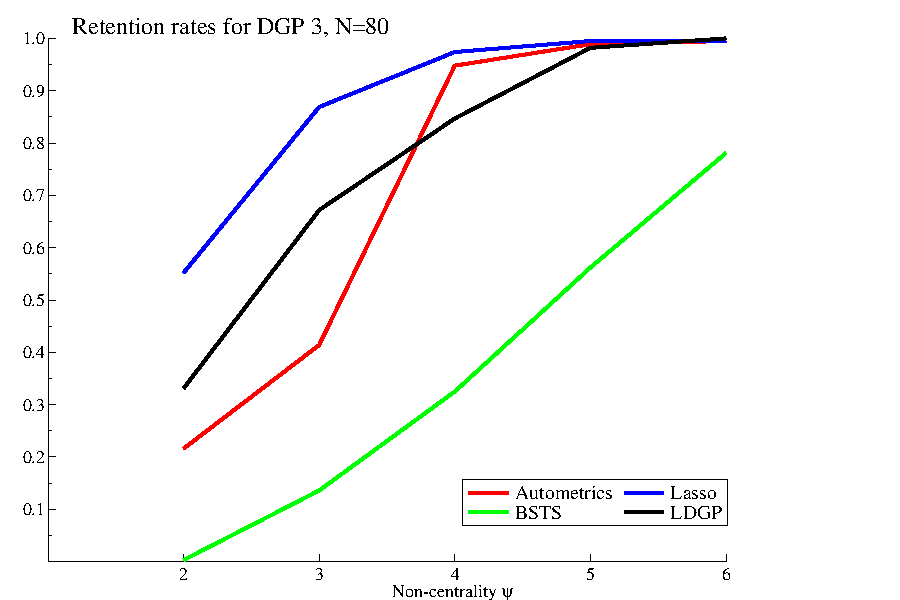
\includegraphics[scale=0.5]{RetRatesDGP3a}
\caption{Retention rates for DGP 3}
\label{fig:RetRatesDGP3a}

\end{minipage}

\end{figure}

\clearpage

The above results show the Lasso consistently achieves the highest potency and has the highest retention rates across all levels of $\psi$ but also has by far the highest gauge. Autometrics selects relevant regressors at a level which is generally similar to the theoretical retention probability (with a couple of exceptions) and does nearly as well as the Lasso when $\psi>4$. In comparison to Lasso and Autometrics, BSTS does not fare well when selecting relevant variables, even for variables with high values of $\psi$. Retention rates and potency measures do not change drastically between $N<T$ and $N>T$ when $\psi>4$, but results for lower values of $\psi$ vary quite significantly. 

BSTS consistently achieves the lowest gauge but its low potency and retention rates indicate that it tends to select very sparse models in general. Note that when conducting the experiments, various priors were tested but this did not seem to have an impact on the results for BSTS. The gauge for Lasso is generally very high and in the range of $0.12$ to $0.22$, which along with the high levels of potency indicate that it selects models which include a lot of variables. In all of the six experiments, Autometrics has a gauge close to the significance level $\alpha = 0.01$, however in DGP 2 with $\psi = 2$, the gauge is slightly higher at $0.029$ probably because it misses some relevant variables with such low non-centralities. It could also possibly correspond to a `bad draw' due to the fact that fixed regressors are used. 

The RCMSE results are most easily interpreted by the graphs, which show that the results vary depending on values of $\psi$. As can be seen in Figures \ref{RCMSECase1a} and \ref{fig:CMSEDGP3a}, Autometrics performs well for high values of $\psi$. Figure \ref{fig:CMSEDGP3a} shows that Lasso and BSTS increasingly struggle as $\psi$ rises. Results are mixed in Figure \ref{fig:RCMSECase2a}, where there is a low non-centrality of $\psi=2$. Note that the spike in RCMSE for $x_{2}$ in Autometrics could be due to the fact that fixed regressors are used. 

Both the Lasso and Autometrics have results similar to, or better than, the benchmark when examining the potency and retention rates. As mentioned, across the board, the Lasso has high potencies and high gauges, meaning that overall there is less `selection' going on. It is a different story when examining the RCMSE results however; Autometrics is much closer to the benchmark (except in the case where $\psi=2$ where results are varied). This means the costs of inference are high in Lasso and BSTS.

The five biggest takeaways from this set of experiments are:
\begin{enumerate}
\item Autometrics consistently has a gauge close to the significance level and retention rates/potencies close to the theoretical retention probabilities.
\item The Lasso scores high for successfully retaining relevant variables, but taken next to the gauges, this is less impressive.
\item BSTS selects models which are very sparse, which is seen clearly through its extremely low measures for gauge, and relatively low levels of potency.
\item The costs of inference vary with $\psi$, but generally are quite low with Autometrics, but high for both the Lasso and BSTS.
\item The huge differences in gauge between the Lasso and BSTS make comparisons using just these two measures impossible. It is infeasible to derive a `gauge-corrected' potency that would make comparisons meaningful.
\end{enumerate}



\subsection{Correlation Between Relevant Regressors}

The second set of experiments considers several cases where there is correlation between the relevant regressors. There are two different DGPs considered, which again vary according to their coefficients $\beta_{1},...,\beta_{5}$ and therefore their respective non-centralities. In both DGPs $\beta_{0}=1$ and $\delta = 0.5$. $\beta_{1},...,\beta_{5}$ have been chosen so that the non-centralities in this set of experiments are in line with those in the first set of experiments, making the results comparable. In all experiments fixed regressors are used. As in the first set of experiments, the two DGPs are nested in two different GUMs with $N=80$ and $N=120$. In all experiments, $T=100$. Thus, there are four separate experiments performed and reported on.   Let $\textbf{x}_{t}'=(x_{1,t},...,x_{N,t})$. The DGPs take the following form: 
$$y_{t}=\beta_{0} + \delta y_{t-1}+\beta_{1}x_{1,t}+\beta_{2}x_{2,t}+ \beta_{3}x_{3,t}+ \beta_{4}x_{4,t}+ \beta_{5}x_{5,t} + \epsilon_{t}$$
$$\epsilon_{t} \sim \mathsf{IN}[0,1] $$
 $$\textbf{x}_{t} \sim \mathsf{IN}_{N} [0,\Omega]$$
with $\omega_{kk} = 1 $, $\omega_{jk} = 0.9 $ for $j \neq k$, $j,k \leq 5$ and $\omega_{jk} = 0 $ elsewhere. Due to the correlation between regressors, it is difficult to derive a formula which analytically gives the relationship between $\psi_{k}$, $\sigma_{\widehat{\beta}_{k}}$, and $t_{\beta_{k}}$. However, $\psi_{k}$ can also be expressed as $\mathsf{E}$[$t_{\widehat{\beta}_{k}}$]. Thus the $\beta_{k}$s in this set of experiment are set such that the average $t$-statistic for variable $x_{k}$ across simulations is equal to the desired $\psi$. More explicitly:
$$\psi_{k} = \mathsf{E}[t_{\widehat{\beta}_{k}}] = \frac{1}{1000}\sum_{i=1}^{1000}t_{\widehat{\beta}_{k},i}$$
where $t_{\widehat{\beta}_{k},i}$ is the calculated $t$-statistic for $\widehat{\beta}_{k}$ in simulation $i$. Table \ref{DGPs4and5} describes the two DGPs considered.
%TABLE DGPs of experiments including orthogonal variables
\begin{table}[h]
\centering
\begin{tabular}{c|c|c|c|c|c|c}

&  &$x_{1}$ &$x_{2}$ &$x_{3}$ &  $x_{4}$ & $x_{5}$  \\
\hline
\textbf{DGP 4} & $\beta_{k}$  & 0.58 &0.84 &1.25 &  1.55 & 1.75 \\

 	& $\psi_{k}$ &2 &3 &4 &5 &6 \\
\hline
\textbf{DGP 5} & $\beta_{k}$  & -0.58 &0.84 &-1.25 &  1.55 &-1.75 \\

 	& $\psi_{k}$  &-2 &3 &-4 &5 &-6 \\

    
\end{tabular}
\caption{DGP specification for experiments with correlation between relevant regressors}
\label{DGPs4and5}
\end{table} 

When the regressors are not orthogonal, as explained, simply using 1-cut selection on the DGP is not a feasible baseline. The `best case scenario' then is doing selection on the DGP using the algorithms themselves. These results capture how effective the algorithm is in the case where the GUM includes exactly the correct regressors. The difference between the RCMSE from selection on the DGP and selection from the GUM is therefore a measure of the costs of inference. 

%For CMSE - no selection on LDGP is benchmark. 




Tables \ref{DGP4GP} and \ref{tDGP4RR} report the gauge, potency and retention rates for DGP 4, and include results when selecting from the DGP for each algorithm. Tables \ref{DGP5GP} and \ref{DGP5RetRates} do the same for DGP 5. Tables \ref{DGP4CMSE} and \ref{LDGP5CMSE} report RCMSE results. The lowest gauge, highest potency, and lowest RCMSE are in bold. Figures \ref{fig:RetRatesDGP4a}-\ref{fig:CMSEDGP5a} graph the results. Figures \ref{fig:CMSEDiffDGP4a} and \ref{fig:CMSEDiffDGP5a} graph the differences between RCMSE for each algorithm and their base line, and thus give an indication of the costs of inference for each of the algorithms.
% Table generated by Excel2LaTeX from sheet 'GPDGP4'
\begin{table}[h]
  \centering
\begin{tabular}{r|r|r|r|r}

         & \multicolumn{2}{|c|}{\textbf{$N=80$}} & \multicolumn{2}{|c}{\textbf{$N=120$}} \\
            & Potency           & Gauge           & Potency            & Gauge           \\
          \hline
    \textbf{Autometrics} & 0.777 & 0.014 & 0.769 & 0.013 \\
    \textit{from DGP} & 0.797 &       & 0.797 &  \\
    \hline
    \textbf{Lasso} & \textbf{0.993} & 0.108 & \textbf{0.993} & 0.077 \\
    \textit{from DGP} & 0.994 &       & 0.994 &  \\
    \hline
    \textbf{BSTS} & 0.690 & \textbf{0.000} & 0.677 & \textbf{0.000} \\
    \textit{from DGP} & 0.784 &       & 0.784 &  \\

    \end{tabular}%
      \caption{Gauge and potency for DGP 4}
  \label{DGP4GP}%
  
\end{table}%
% Table generated by Excel2LaTeX from sheet 'RetRatesChartDGP4'
\begin{table}[h]
  \centering

    \begin{tabular}{r|r|rrrrr}

          & \boldmath{}\textbf{$\psi$}\unboldmath{} & 2     & 3     & 4     & 5     & 6 \\
          \hline

          & $\textsf{P}_{0.01}$ & 0.266 & 0.645 & 0.914 & 0.990 & 0.999  \\
          \hline
    $\bm{N=80} $& \textbf{Autometrics} & 0.333 & 0.568 & 0.988 & 0.998 & 0.998 \\
    \textbf{} & \textbf{Lasso} & \textbf{0.977} & \textbf{0.990} & \textbf{1.000} & \textbf{1.000} & \textbf{1.000} \\
    \textbf{} & \textbf{BSTS} & 0.179 & 0.340 & 0.949 & 0.993 & 0.991 \\
    \hline
   $ \bm{N=120}$ & \textbf{Autometrics} & 0.316 & 0.611 & 0.923 & 0.996 & 0.999 \\
    \textbf{} & \textbf{Lasso} & \textbf{0.968} & \textbf{0.998} & \textbf{1.000} & \textbf{1.000} & \textbf{1.000} \\
    \textbf{} & \textbf{BSTS} & 0.155 & 0.369 & 0.874 & 0.988 & 0.999 \\
    \hline
    \textbf{From DGP} & \textbf{Autometrics} & 0.330 & 0.723 & 0.934 & 0.996 & 1.000 \\
          & \textbf{Lasso} & 0.979 & 0.993 & 1.000 & 1.000 & 1.000 \\
          & \textbf{BSTS} & 0.344 & 0.589 & 0.990 & 0.999 & 0.998 \\

    \end{tabular}%
      \caption{Retention rates for DGP 4, including from DGP}
  \label{tDGP4RR}%
\end{table}%


% Table generated by Excel2LaTeX from sheet 'GPDGP5'
\begin{table}[htbp]
  \centering

    \begin{tabular}{r|r|r|r|r}

         & \multicolumn{2}{|c|}{\textbf{$N=80$}} & \multicolumn{2}{|c}{\textbf{$N=120$}} \\
            & Potency           & Gauge           & Potency            & Gauge           \\
          \hline
    \textbf{Autometrics} & \textbf{0.716} & 0.014 & \textbf{0.719} & 0.014 \\
    \textit{from DGP} & 0.775 &       & 0.775 &  \\
    \hline
    \textbf{Lasso} & 0.429 & 0.088 & 0.374 & 0.057 \\
    \textit{from DGP} & 0.986 &       & 0.986 &  \\
    \hline
    \textbf{BSTS} & 0.531 & \textbf{0.000}   & 0.439 &\textbf{0.000} \\
    \textit{from DGP} & 0.675 &       & 0.675 &  \\

    \end{tabular}%
      \caption{Gauge and potency for DGP 5}
  \label{DGP5GP}%
\end{table}%






% Table generated by Excel2LaTeX from sheet 'RetRatesDGP5Chart'
\begin{table}[htbp]
  \centering

    \begin{tabular}{r|r|rrrrr}

          & \boldmath{}\textbf{$\psi$}\unboldmath{} & -2    & 3     & -4    & 5     & -6 \\
          \hline

        & $\mathsf{P}_{0.01}$ & 0.266 & 0.645 & 0.914 & 0.990 & 0.999  \\
        \hline
    $\bm{N=80} $& \textbf{Autometrics} & \textbf{0.255} & \textbf{0.355} & 0.981 & \textbf{0.996} & 0.994 \\
    \textbf{} & \textbf{Lasso} & 0.065 & 0.013 & \textbf{0.984} & 0.095 & \textbf{0.988} \\
    \textbf{} & \textbf{BSTS} & 0.022 & 0.056 & 0.798 & 0.827 & 0.951 \\
    \hline
    $\bm{N=120}$ & \textbf{Autometrics} & \textbf{0.290} & \textbf{0.482} & \textbf{0.841} & \textbf{0.984} & \textbf{1.000} \\
    \textbf{} & \textbf{Lasso} & 0.254 & 0.007 & 0.590 & 0.019 & 0.998 \\
    \textbf{} & \textbf{BSTS} & 0.054 & 0.061 & 0.353 & 0.727 & 0.999 \\
    \hline
    \textbf{From DGP} & \textbf{Autometrics} & 0.336 & 0.631 & 0.925 & 0.981 & 1.000 \\
          & \textbf{Lasso} & 0.967 & 0.963 & 1.000 & 1.000 & 1.000 \\
          & \textbf{BSTS} & 0.150 & 0.267 & 0.974 & 0.989 & 0.995 \\
 
    \end{tabular}%
      \caption{Retention Rates for DGP 5, including from DGP}
  \label{DGP5RetRates}%
\end{table}%



% Table generated by Excel2LaTeX from sheet 'CMSEChartDGP4'
\begin{table}[htbp]
  \centering

   \begin{tabular}{r|r|rrrrrr}

          &       & $y_{t-1}$ & $x_{1}$ & $x_{2}$ & $x_{3}$ & $x_{4}$ & $x_{5}$ \\
          & $\delta/\beta_{k}$ &   0.5 & 0.58 &0.84 &1.25 &  1.55 & 1.75  \\
           \hline
    $\bm{N=80} $& \textbf{Autometrics} & \textbf{0.017} & 0.438 & 0.423 & 0.277 & 0.377 & 0.377 \\
    \textbf{} & \textbf{Lasso} & 0.038 & \textbf{0.279} & \textbf{0.339} & \textbf{0.259} & \textbf{0.292} & \textbf{0.307} \\
    \textbf{} & \textbf{BSTS} & 0.024 & 0.441 & 0.572 & 0.448 & 0.624 & 0.541 \\
    \hline
    $\bm{N=120}$ & \textbf{Autometrics} & \textbf{0.016} & 0.432 & 0.332 & 0.431 & 0.405 & \textbf{0.342} \\
    \textbf{} & \textbf{Lasso} & 0.038 & \textbf{0.272} & \textbf{0.314} & \textbf{0.333} &\textbf{ 0.313} & 0.354 \\
    \textbf{} & \textbf{BSTS} & 0.020 & 0.530 & 0.555 & 0.606 & 0.626 & 0.499 \\
    \hline
    \textbf{From DGP} & \textbf{Autometrics} & 0.016 & 0.442 & 0.317 & 0.366 & 0.364 & 0.326 \\
          & \textbf{Lasso} & 0.021 & 0.266 & 0.329 & 0.255 & 0.286 & 0.297 \\
          & \textbf{BSTS} & 0.026 & 0.395 & 0.504 & 0.375 & 0.484 & 0.432 \\

    \end{tabular}%
      \caption{RCMSE for DGP 4, including baseline}
  \label{DGP4CMSE}%
\end{table}%


% Table generated by Excel2LaTeX from sheet 'CMSEDGP5Chart'
\begin{table}[htbp]
  \centering

    \begin{tabular}{r|r|rrrrrrr}

          &       & $y_{t-1}$ & $x_{1}$ & $x_{2}$ & $x_{3}$ & $x_{4}$ & $x_{5}$ &  \\

         & $\delta/\beta_{k}$ &   0.5 & -0.58 &0.84 &-1.25 &  1.55 & -1.75  \\
         \hline
    $\bm{N=80} $& \textbf{Autometrics} & 0.334 & \textbf{0.281} & \textbf{0.316} & \textbf{0.287} & \textbf{0.325} & \textbf{0.258} &  \\
    \textbf{} & \textbf{Lasso} & 0.120 & 0.463 & 0.656 & 0.778 & 1.074 & 1.225 &  \\
    \textbf{} & \textbf{BSTS} & \textbf{0.078} & 0.288 & 0.527 & 0.446 & 0.572 & 0.571 &  \\
    \hline
    $\bm{N=120}$ & \textbf{Autometrics} & 0.273 & \textbf{0.292} & \textbf{0.303} & \textbf{0.296} & \textbf{0.341} & \textbf{0.257} &  \\
    \textbf{} & \textbf{Lasso} & 0.226 & 0.424 & 0.554 & 1.030 & 1.029 & 0.955 &  \\
    \textbf{} & \textbf{BSTS} & \textbf{0.097} & 0.405 & 0.510 & 0.603 & 0.722 & 0.496 &  \\
    \hline
    \textbf{From DGP} & \textbf{Autometrics} & 0.051 & 0.342 & 0.239 & 0.330 & 0.334 & 0.330 &  \\
          & \textbf{Lasso} & 0.052 & 0.286 & 0.362 & 0.266 & 0.307 & 0.326 &  \\
          & \textbf{BSTS} & 0.071 & 0.342 & 0.482 & 0.384 & 0.411 & 0.408 &  \\

    \end{tabular}%
      \caption{RCMSE for DGP 5, including from DGP}
  \label{LDGP5CMSE}%
\end{table}%






\begin{figure}

\begin{minipage}{.5\textwidth}
\centering
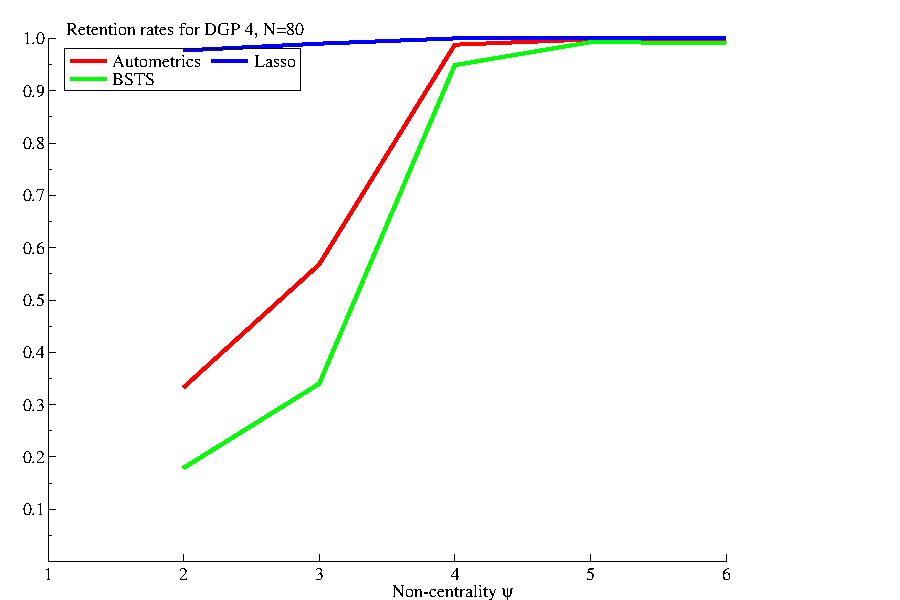
\includegraphics[scale=0.5]{RetRatesDGP4a}
\caption{Retention rates DGP 4 \newline $N=80$}
\label{fig:RetRatesDGP4a}
\end{minipage}%
\begin{minipage}{.5\textwidth}
\centering
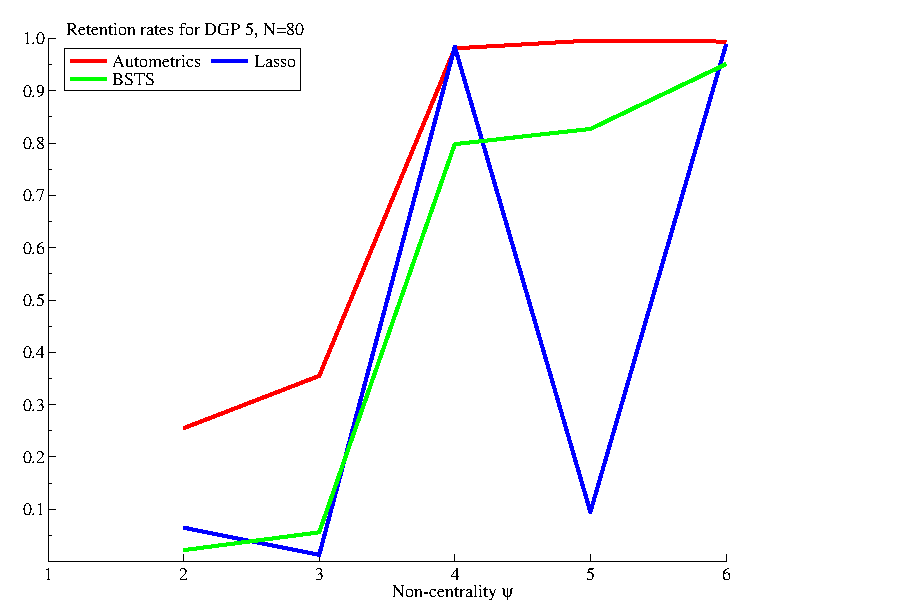
\includegraphics[scale=0.5]{RetRatesDGP5a}
\caption{Retention Rates DGP 5 \newline $N=80$}
\label{fig:RetRatesDGP5a}

\end{minipage}

\end{figure}

\begin{figure}

\begin{minipage}{.5\textwidth}
\centering
\includegraphics[scale=0.5]{RCMSEDGP4a}
\caption{RCMSE for DGP 4 \newline $N=80$}
\label{fig:CMSEDGP4a}
\end{minipage}%
\begin{minipage}{.5\textwidth}
\centering
\includegraphics[scale=0.5]{RCMSEDGP5a}
\caption{RCMSE for DGP 5 \newline $N=80$}
\label{fig:CMSEDGP5a}

\end{minipage}

\end{figure}

\begin{figure}

\begin{minipage}{.5\textwidth}
\centering
\includegraphics[scale=0.5]{RCMSEDiffDGP4a}
\captionsetup{justification=centering}
\caption{RCMSE Differences for DGP 4 \newline $N=80$}
\label{fig:CMSEDiffDGP4a}
\end{minipage}%
\begin{minipage}{.5\textwidth}
\centering
\includegraphics[scale=0.5]{RCMSEDiffDGP5a}
\captionsetup{justification=centering}
\caption{RCMSE Differences for DGP 5 \newline $N=80$}
\label{fig:CMSEDiffDGP5a}

\end{minipage}

\end{figure}

\clearpage
%Note that this section only examines results within the set of experiments where there is correlation between relevant regressors; analysis and comparison across the three sets of experiments will be discussed later on. 

When considering DGP 4 results, when $\psi_{k} > 0, \forall k$, the Lasso has both the highest measures of potency and gauge. BSTS has the lowest gauge and Autometric's gauge is close to the significance level $\alpha$. Going from $N<T$ to $N>T$ in most cases does not have a big impact on the results. Both Autometrics and the Lasso have retention rates similar to their benchmark, while the benchmark for BSTS gives quite different results. The graph for the RCMSE differences is interesting, and shows there are almost no costs of search for the Lasso, and for Autometrics there are in fact negative costs of search, meaning that sometimes parameter estimates are even more accurate than in the theoretical best case scenario. This is likely due to adventitiously selecting irrelevant variables which partly proxy a relevant variable which has not been selected, which results in a smaller error variance.

When looking at DGP 5, it is clear that the algorithms struggle to varying degrees with alternating signs. This is particularly true for the Lasso, with retention rates on regressors with $\psi>0$ being very low, irrespective of their magnitude, when the largest $\psi$ in the experiment is negative. The search costs of the Lasso also increase with $|\psi|$. The results for the gauge are similar to previous experiments; the gauge for BSTS is low in every experiment, the gauge for Autometrics is slightly higher than the significance level $\alpha$, and the gauge for the Lasso varies across the experiments. The costs of search for both Autometrics and BSTS, as measured by the RCMSE differences, are quite low. 

Comparing the results from DGP 4 to DGP 5 is striking. While intuitively and theoretically the DGPs have nearly identical properties, the actual results vary drastically. Thinking about non-centrality as the signal-to-noise ratio, whether a variable has a positive or negative non-centrality should not have an impact on how often it is selected by an algorithm; it is the magnitude of the the signal-to-noise ratio, $|\psi|$, which should influence an algorithm's ability to select that variable. Indeed, in the case of orthogonal variables alternating signs did not result in potency and retention rate measures which were notably different from cases where the signs were all the same. 

It is immediately clear however that something peculiar is going on with DGP 5 when the signs are alternating. DGP 4 has retention rates as expected are increasing with $\psi$. In DGP 5 while both Autometrics and BSTS have higher retention rates as $|\psi|$ rises, the Lasso struggles to select either of the regressors with $\psi>0$. It should also be noted that while the retention rates do increase with $|\psi|$ for Autometrics and BSTS, the increase is not at all `uniform' and both Autometrics and BSTS are more successful at selecting variables with $\psi<0$. The RCMSE results illustrate the parameter estimates also vary across the DGPs. In DGP 4, the Lasso has the lowest RCMSE for all variables, while it has the highest RCMSEs for all variables in DGP 5. Furthermore, the RCMSEs increase with $\psi$ for the Lasso with alternating signs. 

The reason why the Lasso has such difficulty selecting the regressors with negative signs is due to the nature of the search its algorithm uses to identify non-zero coefficients. The algorithm identifies the regressor which is `most significant' and shrinks the coefficients of regressors which are highly correlated with the identified regressor to zero. Certain implementations of the Lasso have built in features to account for this when the coefficients of the correlated regressors have the same sign (i.e. see Hastie and Zou (2005)) but no algorithm exists to account for regressors which have coefficients with opposite signs. In the case of DGP 5, the Lasso (correctly) identifies $x_{5}$ with $\psi_{5} = -6$ as the most significant, and since $x_{5}$ is highly correlated with $x_{1},...,x_{4}$, it shrinks their coefficients to zero. Because the Lasso allows for variables which are significant `in the same direction' (i.e. in this case negatively significant), to be effectively `re-added', variables $x_{1}$ and $x_{3}$ which have respective non-centralities of -2 and -4 are selected, but there is no mechanism for $x_{2}$ and $x_{4}$ with their positive coefficients to be `reconsidered' for selection. If it was the case that the most significant variable had a positive coefficient, then any variables with negative coefficients would be shrunk to zero and not selected. That is, negative coefficients and positive correlations are isomorphic to positive coefficients and negative correlations, so this result would also hold if it parameter signs were switched.

The biggest takeaways from this second set of experiments are:
\begin{enumerate}
\item Selection when signs alternate produces remarkably different results, especially for the Lasso. 
%This is likely due to the nature by which Lasso's algorithm works; omitting one of a pair of 
\item When $\psi_{k} > 0 \ \forall \ k$ the Lasso selects a lot of both relevant and irrelevant variables, BSTS does not select many of either, and Autometrics is somewhere in the middle. 
\item In terms of their RCMSEs, the behaviour of Autometrics commencing from the GUM is relatively similar to starting from the DGP. The retention rates for relevant variables in both these cases are close to the theory-derived retention probabilities.
\item Remarkably, across all experiments, there is little difference in the performance of Autometrics between $N<T$ and $N>T$ ($N=80$ and $N=120$). 
\item As found in the previous set of experiments, search costs for Autometrics can sometimes be negative.
\item The RCMSEs for Autometrics are relatively constant across all $\psi$ and for the Lasso and BSTS they are not. 
\end{enumerate}



\subsection{Correlation Between all Regressors}


The third set of experiments considers several cases where there is correlation between all regressors. There are two different DGPs considered, which again vary according to the coefficients $\beta_{1},...,\beta_{5}$ and therefore their respective non-centralities. Fixed regressors are used in all experiments. These two DGPs are nested, as previously, in two different GUMs with $N=80$ and $N=120$. In all experiments, $T=100$. There are four separate experiments performed and reported on. Let $\textbf{x}_{t}'=(x_{1,t},...,x_{N,t})$. The DGPs take the following form: 
$$y_{t}=\beta_{0} + \delta y_{t-1}+\beta_{1}x_{1,t}+\beta_{2}x_{2,t}+ \beta_{3}x_{3,t}+ \beta_{4}x_{4,t}+ \beta_{5}x_{5,t} + \epsilon_{t}$$
$$\epsilon_{t} \sim \mathsf{IN}[0,1] $$
 $$\textbf{x}_{t} \sim \mathsf{IN}_{N}[0,\Omega]$$
with $\omega_{kk} = 1 $, $\omega_{jk} = 0.8 $ for $k \neq j $. The biggest difference between this set of experiments and previous set is that here $\Omega$ is a full $N \times N$ matrix. As with the second set of experiments,  determining the relationship between $\psi_{k}$, $\beta_{k}$ and $\sigma_{\hat{\beta_{k}}}$ is difficult to do analytically because of the correlation structure. Thus $\beta_{1},...,\beta_{5}$ in this set of experiment are set such that the average $t$-statistic for variable $x_{k}$ across simulations aligns with the non-centralities in the previous experiments. More explicitly:
$$\psi_{k} = \mathsf{E}[t_{\widehat{\beta}_{k}}] = \frac{1}{1000}\sum_{i=1}^{1000}t_{\widehat{\beta}_{k},i}$$
where $t_{\widehat{\beta}_{k},i}$ is the calculated $t$-statistic for $\widehat{\beta}_{k}$ in simulation $i$. Table \ref{DGP67} describes the two DGPs considered, with the $\beta_{k}$s that correspond to the desired $\psi_{k}$s. 



The following table describes the two DGPs considered, from hereon referred to as DGP 6 and 7:


%TABLE DGPs of experiments including orthogonal variables
\begin{table}[h]



\centering
\begin{tabular}{c|c|c|c|c|c|c}

&  &$x_{1}$ &$x_{2}$ &$x_{3}$ &  $x_{4}$ & $x_{5}$  \\
\hline
\textbf{DGP 6} & $\beta_{k}$  & 0.4&0.6 &0.9&1.1  &1.25  \\

 	& $\psi_{k}$  &2 &3 &4 &5 &6 \\
\hline
\textbf{DGP 7} & $\beta_{k}$  & -0.4&0.6 &-0.9&1.1  &-1.25 \\

 	& $\psi_{k}$ &-2 &3 &-4 &5 &-6 \\

    
\end{tabular}
\caption{DGP specification for experiments with correlation between all regressors}
\label{DGP67}
\end{table} 
The following tables report the potency, gauge, retention rates and RCMSE for DGP 6 and DGP 7. The lowest gauge, highest potency and lowest RCMSE are in bold. Again in this set of experiments the significance level for Autometrics was set to $\alpha= 0.01$. The results are also graphed. 
\\
% Table generated by Excel2LaTeX from sheet 'DGP6GP'
\begin{table}[htbp]
  \centering

    \begin{tabular}{r|r|r|r|r}

         & \multicolumn{2}{|c|}{$N=80$} & \multicolumn{2}{|c}{$N=120$}  \\
            & Potency           & Gauge           & Potency            & Gauge           \\
          \hline
    \textbf{Autometrics} & 0.736 & 0.016 & 0.718 & 0.015 \\
    \textit{from DGP} & 0.798 &       & 0.798 &  \\
    \hline
    \textbf{Lasso} & \textbf{0.909} & 0.182 & \textbf{0.894} & 0.131 \\
    \textit{from DGP} & 0.993 &       & 0.993 &  \\
    \hline
    \textbf{BSTS} & 0.653 & \textbf{0.004} & 0.631 & \textbf{0.005} \\
    \textit{from DGP} & 0.764 &       & 0.764 &  \\

    \end{tabular}%
      \caption{Gauge and potency for DGP 6}
  \label{DGP6GP}%
\end{table}%




% Table generated by Excel2LaTeX from sheet 'RetRatesDGP6Chart'
\begin{table}[htbp]
  \centering

    \begin{tabular}{r|r|rrrrr}

          & \boldmath{}\textbf{$\psi$}\unboldmath{} & 2    & 3     & 4    & 5     & 6 \\
          \hline

          & $\mathsf{P}_{0.01}$ & 0.266 & 0.645 & 0.914 & 0.990 & 0.999  \\
          \hline
    $\bm{N=80}$ & \textbf{Autometrics} & 0.262 & 0.439 & 0.985 & 0.996 & 0.996 \\
    \textbf{} & \textbf{Lasso} & \textbf{0.766} & \textbf{0.778} & \textbf{1.000} & \textbf{1.000} & \textbf{1.000} \\
    \textbf{} & \textbf{BSTS} & 0.116 & 0.251 & 0.923 & 0.984 & 0.990 \\
    \hline
    $\bm{N=120}$ & \textbf{Autometrics} & 0.212 & 0.524 & 0.890 & 0.966 & 0.999 \\
    \textbf{} & \textbf{Lasso} & \textbf{0.560} & \textbf{0.924} & \textbf{0.991} & \textbf{0.998} & \textbf{0.999} \\
    \textbf{} & \textbf{BSTS} & 0.093 & 0.285 & 0.810 & 0.971 & 0.997 \\
    \hline
    \textbf{From DGP} & \textbf{Autometrics} & 0.327 & 0.729 & 0.938 & 0.995 & 1.000 \\
          & \textbf{Lasso} & 0.969 & 0.994 & 1.000 & 1.000 & 1.000 \\
          & \textbf{BSTS} & 0.281 & 0.554 & 0.990 & 0.998 & 0.999 \\

    \end{tabular}%
      \caption{Retention Rates for DGP 6}
  \label{DGP6RetRates}%
\end{table}%

% Table generated by Excel2LaTeX from sheet 'CMSEDGP6Chart'
\begin{table}[htbp]
  \centering

    \begin{tabular}{r|r|rrrrrr}
  
          &       & $y_{t-1}$ & $x_{1}$ & $x_{2}$ & $x_{3}$ & $x_{4}$ & $x_{5}$ \\

          &   $\delta/\beta_{k} $   & 0.5 & 0.4&0.6 &0.9&1.1  &1.25  \\
          \hline
    $\bm{N=80}$ & \textbf{Autometrics} & \textbf{0.025} & 0.318 & \textbf{0.313} & \textbf{0.190} & \textbf{0.241} & \textbf{0.250} \\
    \textbf{} & \textbf{Lasso} & 0.041 & \textbf{0.230} & 0.347 & 0.257 & 0.349 & 0.315 \\
    \textbf{} & \textbf{BSTS} & 0.036 & 0.318 & 0.404 & 0.386 & 0.386 & 0.348 \\
    \hline
    $\bm{N=120}$ & \textbf{Autometrics} & \textbf{0.023} & 0.329 & \textbf{0.227} & \textbf{0.263} & \textbf{0.254} & \textbf{0.232} \\
    \textbf{} & \textbf{Lasso} & 0.033 & \textbf{0.254 }& 0.313 & 0.376 & 0.462 & 0.389 \\
    \textbf{} & \textbf{BSTS} & 0.026 & 0.306 & 0.370 & 0.430 & 0.428 & 0.346 \\
    \hline
    \textbf{From DGP} & \textbf{Autometrics} & 0.024 & 0.307 & 0.219 & 0.259 & 0.255 & 0.230 \\
          & \textbf{Lasso} & 0.029 & 0.192 & 0.234 & 0.182 & 0.204 & 0.211\\
          & \textbf{BSTS} & 0.036 & 0.275 & 0.361 & 0.258 & 0.337 & 0.314 \\
 
    \end{tabular}%
      \caption{RCMSE for DGP 6}
  \label{DGP6CMSE}%
\end{table}%


% Table generated by Excel2LaTeX from sheet 'GPDGP7'
\begin{table}[htbp]
  \centering
 
    \begin{tabular}{r|r|r|r|r}

         & \multicolumn{2}{|c|}{$N=80$} & \multicolumn{2}{|c}{$N=120$}  \\
            & Potency           & Gauge           & Potency            & Gauge           \\
          \hline
    \textbf{Autometrics} & 0.718 & 0.014 & 0.707 & 0.014 \\
    \textit{from DGP} & 0.778 &    & 0.778 &  \\
    \hline
    \textbf{Lasso} & \textbf{0.787} & 0.154 & \textbf{0.823} & 0.131 \\
    \textit{from DGP} & 0.986 &    & 0.986 &  \\
    \hline
    \textbf{BSTS} & 0.512 & \textbf{0.001} & 0.401 & \textbf{0.001} \\
    \textit{from DGP} & 0.657 &   & -0.657 &  \\

    \end{tabular}%
     \caption{Gauge and potency for DGP 7}
  \label{DGP7GP}%
\end{table}%


% Table generated by Excel2LaTeX from sheet 'RetRatesDGP7Chart'
\begin{table}[htbp]
  \centering

    \begin{tabular}{r|r|rrrrr}

          & \boldmath{}\textbf{$\psi$}\unboldmath{} & -2    & 3     & -4    & 5     & -6 \\
          \hline

          & $\mathsf{P}_{0.01}$ & 0.266 & 0.645 & 0.914 & 0.990 & 0.999  \\
          \hline
    \textbf{N=80} & \textbf{Autometrics} & 0.230 & 0.380 & 0.988 & 0.993 & 0.998 \\
    \textbf{} & \textbf{Lasso} & \textbf{0.507} & \textbf{0.466} & \textbf{0.999} & \textbf{0.963} & \textbf{1.000} \\
    \textbf{} & \textbf{BSTS} & 0.011 & 0.041 & 0.812 & 0.791 & 0.907 \\
    \hline
    \textbf{N=120} & \textbf{Autometrics} & 0.253 & 0.510 & 0.803 & 0.972 & 0.999 \\
    \textbf{} & \textbf{Lasso} & \textbf{0.603} & \textbf{0.683} & \textbf{0.904} & \textbf{0.926} & \textbf{1.000} \\
    \textbf{} & \textbf{BSTS} & 0.037 & 0.051 & 0.303 & 0.641 & 0.971 \\
    \hline
    \textbf{From DGP} & \textbf{Autometrics} & 0.330 & 0.649 & 0.931 & 0.980 & 1.000 \\
          & \textbf{Lasso} & 0.964 & 0.967 & 1.000 & 1.000 & 1.000 \\
          & \textbf{BSTS} & 0.103 & 0.242 & 0.965 & 0.983 & 0.993 \\

    \end{tabular}%
     \caption{Retention Rates for DGP 7}
  \label{DGP7RetRates}%
\end{table}%

% Table generated by Excel2LaTeX from sheet 'CMSEDGP7Chart'
\begin{table}[htbp]
  \centering

    \begin{tabular}{r|r|rrrrrr}

          &       & $y_{t-1}$ & $x_{1}$ & $x_{2}$ & $x_{3}$ & $x_{4}$ & $x_{5}$ \\

     &     & 0.5 & -0.4&0.6 &-0.9&1.1  &-1.25  \\
     \hline
    $\bm{N=80}$ & \textbf{Autometrics} & \textbf{0.059} & 0.286 & \textbf{0.267} & \textbf{0.187} & \textbf{0.224} & \textbf{0.246} \\
    \textbf{} & \textbf{Lasso} & 0.078 & 0.257 & 0.415 & 0.330 & 0.514 & 0.532 \\
    \textbf{} & \textbf{BSTS} & 0.111 & \textbf{0.188} & 0.358 & 0.327 & 0.405 & 0.438 \\
    \hline
     $\bm{N=120}$ & \textbf{Autometrics} & \textbf{0.070} & 0.328 & \textbf{0.230} & \textbf{0.221} & \textbf{0.253} &\textbf{ 0.232} \\
    \textbf{} & \textbf{Lasso} & 0.121 & \textbf{0.257} & 0.370 & 0.526 & 0.564 & 0.421 \\
    \textbf{} & \textbf{BSTS} & 0.147 & 0.272 & 0.362 & 0.458 & 0.515 & 0.359 \\
    \hline
    \textbf{From DGP} & \textbf{Autometrics} & 0.059 & 0.246 & 0.168 & 0.237 & 0.236 & 0.232 \\
          & \textbf{Lasso} & 0.059 & 0.205 & 0.256 & 0.190 & 0.216 & 0.229 \\
          & \textbf{BSTS} & 0.084 & 0.236 & 0.344 & 0.281 & 0.294 & 0.298 \\

    \end{tabular}%
      \caption{RCMSE for DGP 7}
  \label{DGP7CMSE}%
\end{table}%













\begin{figure}[h]

\begin{minipage}{.5\textwidth}
\centering
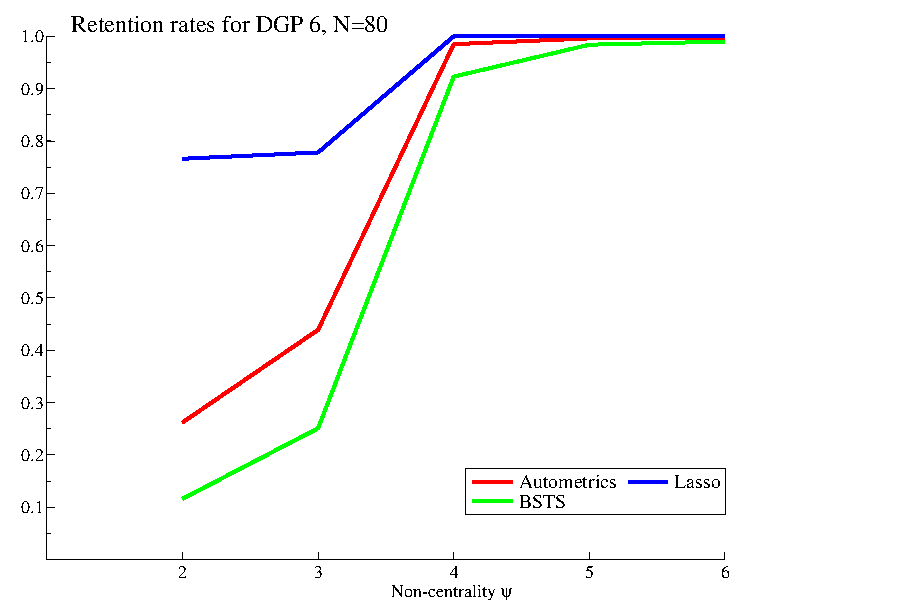
\includegraphics[scale=0.5]{RetRatesDGP6a}
\caption{Retention rates DGP 6 \newline $N=80$}
\label{fig:RetRatesDGP6a}
\end{minipage}%
\begin{minipage}{.5\textwidth}
\centering
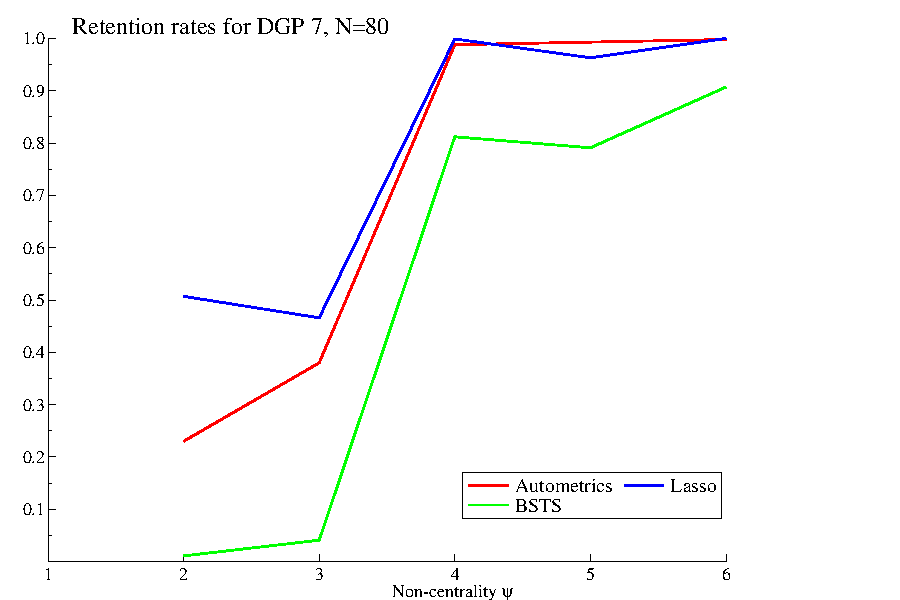
\includegraphics[scale=0.5]{RetRatesDGP7a}
\caption{Retention Rates DGP 7 \newline $N=80$}
\label{fig:RetRatesDGP7a}

\end{minipage}

\end{figure}

\begin{figure}[h]

\begin{minipage}{.5\textwidth}
\centering
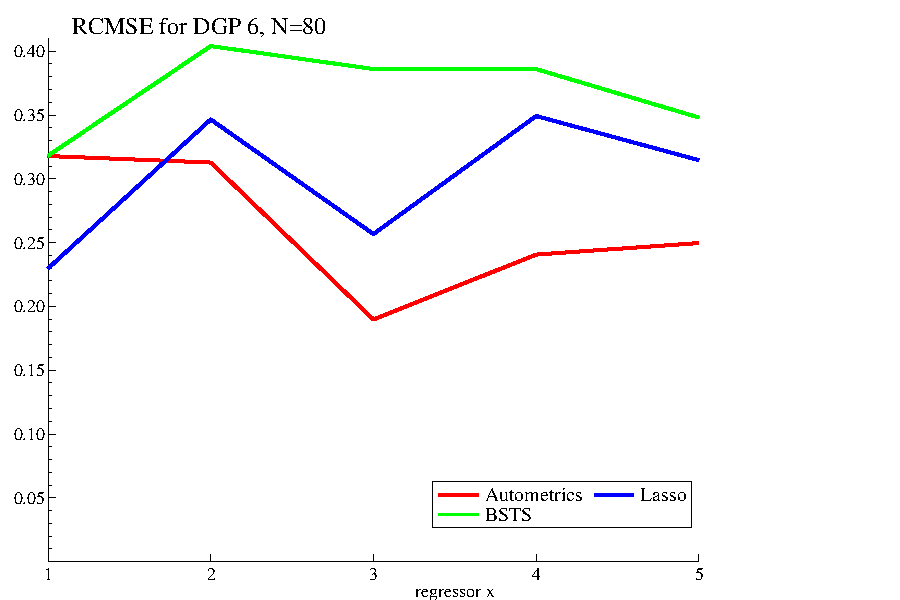
\includegraphics[scale=0.5]{RCMSE-DGP6a}
\caption{RCMSE DGP 6 \newline $N=80$}
\label{fig:CMSEDGP6a}
\end{minipage}%
\begin{minipage}{.5\textwidth}
\centering
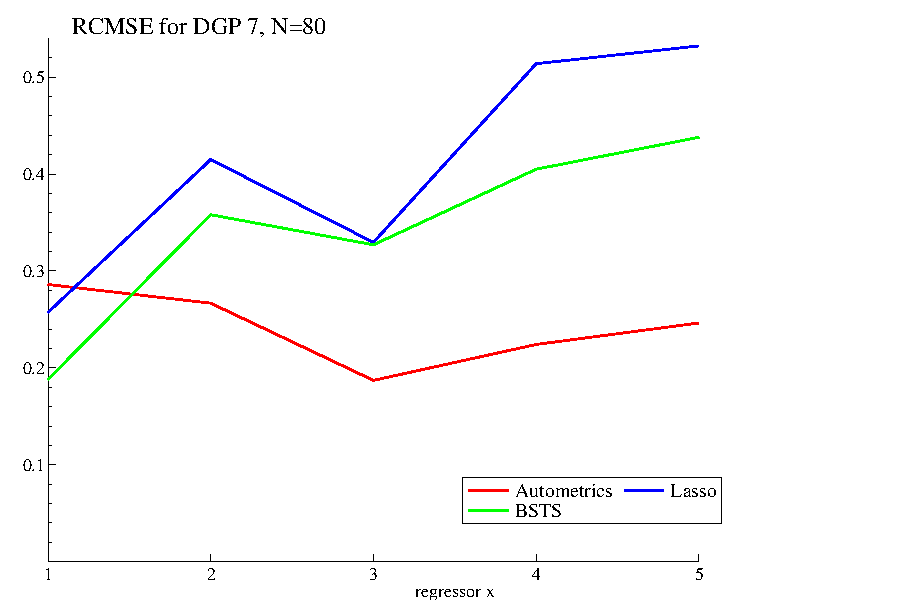
\includegraphics[scale=0.5]{RCMSE-DGP7a}
\caption{RCMSE DGP 7 \newline $N=80$}
\label{fig:CMSEDGP7a}

\end{minipage}

\end{figure}




\begin{figure}[h]

\begin{minipage}{.5\textwidth}
\centering
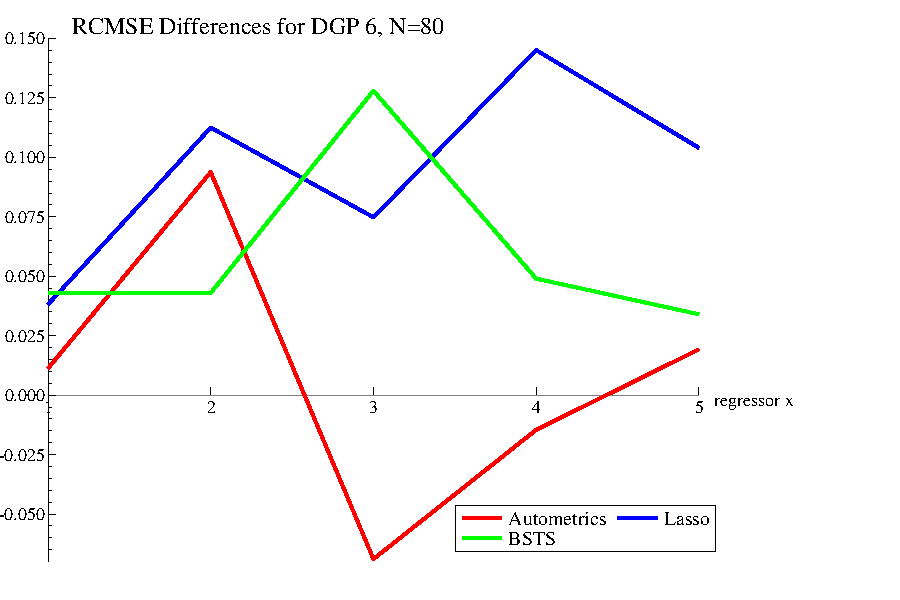
\includegraphics[scale=0.5]{RCMSEDiffDGP6a}
\caption{RCMSE differences DGP 6 \newline $N=80$}
\label{fig:CMSEDGP6a}
\end{minipage}%
\begin{minipage}{.5\textwidth}
\centering
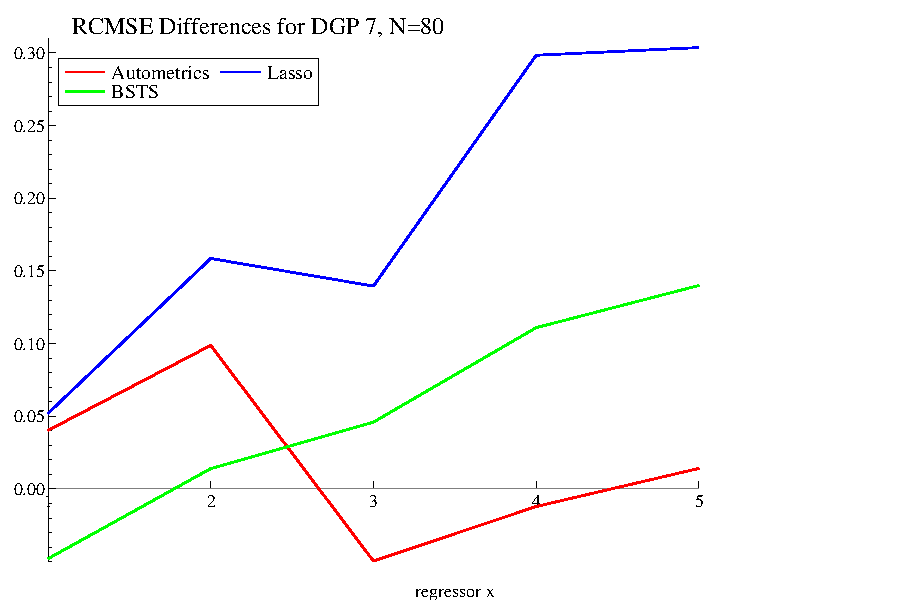
\includegraphics[scale=0.5]{RCMSEDiffDGP7a}
\caption{RCMSE differences DGP 7 \newline $N=80$}
\label{fig:CMSEDGP7a}

\end{minipage}

\end{figure}

\clearpage

First considering the results from DGP 6, the Lasso appears to be effective at identifying relevant variables but also tends to select many irrelevant variables overall, as evidenced by the high gauge. When $\psi>3$, the retention rates for all three algorithms are very high. The gauge for Autometrics is slightly higher than the significance level $\alpha$, and almost 0 for BSTS. The RCMSE are generally highest for BSTS and lowest for Autometrics. Search costs are lowest for Autometrics. 

With the DGP 7 results, the retention rates are similar to those of DGP 6 but different in a subtle and important way. Both the Lasso and BSTS struggle to pick up variables with $\psi>0$. Similarly, the Lasso struggles to estimate the parameters on variables with $\psi>0$. These difficulties are not as pronounced as in the previous set of experiments, but clear nonetheless. While the Lasso and BSTS struggle increasingly to estimate the parameter estimates as $|\psi|$ increases, Autometrics has RCMSEs which are low and consistent for all variables. 

Comparing DGP 6 and DGP 7, several important differences arise. While in theory the DGPs are very similar with almost identical properties, the results vary. The Lasso and BSTS again appear to struggle with alternating signs both in terms of how effectively they pick up relevant variables and how accurate the parameter estimates are. The measures of gauge are consistent across all algorithms in both DGP 6 and DGP 7; again BSTS with the lowest gauge near 0, the Lasso with the highest in the range of 0.13-0.18, and Autometrics in the middle with gauges slightly above the significance level.

An additional observation is that the Lasso struggled less when dealing with alternating signs and all variables correlated in this set of experiments, than it did when only the relevant regressors were correlated in the previous set of experiments. This is likely due to the fact that in this set of experiments the correlation between all variables was $\omega_{jk} = 0.8$ and in the previous set of experiments the correlation between relevant variables was $\omega_{jk} = 0.9$. 

The takeaways from this set of experiments are:
\begin{enumerate}
\item Alternating signs matter a lot for the Lasso, a reasonable amount for BSTS and a little for Autometrics. Note that negative coefficients and positive correlations are isomorphic to positive coefficients and negative correlations, so this result would also hold if it parameter signs were switched.
\item The Lasso is excellent at selecting relevant variables when all the signs are the same, but not very good at excluding irrelevant variables.
\item The gauge for Autometrics is consistently slightly above the significance level for all experiments. 
\item BSTS generally selects very sparse models, which do not include many relevant or irrelevant variables.
\end{enumerate}.

\clearpage
























 








\newpage

\section{Results Summary}

Evaluating the algorithms up until this point has focused on comparing the results from model selection conditional on a known correlation structure between the regressors. Therefore, when thinking about what the results in the previous section say about empirical model selection, the correlation structure of the variables under consideration must be taken into account. For example, if a researcher used Autometrics or the Lasso on a set of orthogonal variables, she would know that the model selected by Autometrics included $\alpha$\% of the irrelevant variables, and the model selected by the Lasso included 15-20\% of the irrelevant variables. Additionally she would know there was a 99\% chance that a variable with a signal-to-noise ratio of 4 was included in the selected model. These statements rely on orthogonality however, and given that the world is dynamic, full of relationships and extremely interdependent, orthogonal results on their own are of limited use. Because a researcher never knows the true DGP, she cannot possibly know what the true correlation structure is. Thus, to truly be able to interpret and say something meaningful about the effectiveness of model selection empirically, it is vital to understand how different `states of nature' influence the results. Since a researcher can never know the true DGP and therefore cannot qualify results in this manner, ideally model selection results should not depend on the correlation structure.

A desirable property of model selection would be for a variable with a given `significance', which can be measured by its non-centrality, to be selected at the same level regardless of the properties of the other variables in the GUM. It is for this reason that in each of the three sets of experiments, $\beta_{1},...,\beta_{5}$ were chosen so that non-centralities are the same and retention rates and RCMSEs are comparable across experiments. Looking at how results vary across the three different correlation structures is therefore a straightforward way to analyze how orthogonality or otherwise influences results across values of $\psi$. Table \ref{tab:SummaryPositive} shows a summary of the results for DGP 3, DGP 4, and DGP 6 for $N=80$. Similarly, Table \ref{tab:SummaryAlt} shows the results for DGPs with alternating signs. Note that results from alternating signs when the regressors are orthogonal are largely the same as when the signs are all the same, and were not reported earlier. 

% Table generated by Excel2LaTeX from sheet 'Allpositive-noformulas'

\begin{landscape}

\begin{table}[htbp]
  \centering

    \begin{tabular}{r|rrr|rrr|rrr}
  & \multicolumn{3}{c|}{\textbf{Autometrics}}  & \multicolumn{3}{c|}{\textbf{Lasso}}                                                   & \multicolumn{3}{c}{\textbf{BSTS}}                        \\ \hline
$\psi$ & Orthogonal & Some Corr & All Corr & Orthogonal & Some Corr & All Corr & Orthogonal & Some Corr                & All Corr \\ \hline
    2     & 0.216 & 0.333 & 0.262 & 0.552 & 0.977 & 0.766 & 0.003 & 0.179 & 0.116 \\
    3     & 0.414 & 0.568 & 0.439 & 0.869 & 0.990  & 0.778 & 0.136 & 0.340  & 0.251 \\
    4     & 0.948 & 0.988 & 0.985 & 0.974 & 1.000     & 1.000     & 0.325 & 0.949 & 0.923 \\
    5     & 0.989 & 0.998 & 0.996 & 0.995 & 1.000     & 1.000     & 0.562 & 0.993 & 0.984 \\
    6     & 0.995 & 0.998 & 0.996 & 0.996 & 1.000     & 1.000     & 0.781 & 0.991 & 0.99 \\
   \hline
    Potency & 0.712 & 0.777 & 0.736 & 0.877 & 0.993 & 0.909 & 0.361 & 0.690 & 0.653 \\
    Gauge & 0.018 & 0.014 & 0.016 & 0.179 & 0.108 & 0.182 & 0.001 & 0.000 & 0.004 \\


 
    \end{tabular}%
 
    \caption{Retention rate, potency and gauge summary results for all positive $\psi$}
     \label{tab:SummaryPositive}%
\end{table}%

% Table generated by Excel2LaTeX from sheet 'Alternating-noformulas'
\begin{table}[htbp]
  \centering

    \begin{tabular}{r|rrr|rrr|rrr}
  & \multicolumn{3}{c|}{\textbf{Autometrics}}  & \multicolumn{3}{c|}{\textbf{Lasso}}                                                   & \multicolumn{3}{c}{\textbf{BSTS}}                        \\ \hline
$\psi$ & Orthogonal & Some Corr & All Corr & Orthogonal & Some Corr & All Corr & Orthogonal & Some Corr                & All Corr \\ \hline

    -2    & 0.240  & 0.255 & 0.230  & 0.608 & 0.065 & 0.507 & 0.007 & 0.022 & 0.011 \\
    3     & 0.476 & 0.355 & 0.380  & 0.74  & 0.013 & 0.466 & 0.043 & 0.056 & 0.041 \\
    -4    & 0.928 & 0.981 & 0.988 & 0.981 & 0.984 & 0.999 & 0.349 & 0.798 & 0.812 \\
    5     & 0.993 & 0.996 & 0.993 & 1.000     & 0.095 & 0.963 & 0.943 & 0.827 & 0.791 \\
    -6    & 0.996 & 0.994 & 0.998 & 0.998 & 0.988 & 1.000     & 0.792 & 0.951 & 0.907 \\
    \hline
    Potency & 0.727 & 0.716 & 0.718 & 0.865 & 0.429 & 0.787 & 0.427 & 0.531 & 0.512 \\
    Gauge & 0.018 & 0.014 & 0.014 & 0.176 & 0.088 & 0.154 & 0.000 & 0.000 & 0.001 \\

    \end{tabular}%
  
    \caption{Retention rate, potency and gauge summary results for alternating $\psi$}
    \label{tab:SummaryAlt}%
\end{table}%

\end{landscape}

These two tables contain many interesting insights. The results for Autometrics do not vary significantly across the different correlation structures, both when $\psi_{k}>0,\forall k$ and when the signs of $\psi$ alternate. As $|\psi|$ increases, correlation matters less and results converge to 1. The gauge is also consistent across correlation structures, fluctuating between 0.014 and 0.018.  The Lasso, on the other hand, exhibits a very different story. While when $\psi_{k}>0, \forall k$, and $\psi>3$ the retention rates are consistent across the correlation structures, this is not the case when the signs are alternating. In fact, in the case of alternating signs, the Lasso picks up variable $x_{k}$ with $\psi_{k}=3$, 74\% of the time when the regressors are orthogonal, compared to 1\% of the time when there is correlation between the relevant regressors, and 46\% of the time when there is correlation between all regressors. The gauge in the Lasso experiments is also remarkably varied, ranging between 0.09 and 0.18. These discrepancies and their implications are substantial. The same is true but to a lesser extent for BSTS where there is notable variation in retention rates across the three correlation structures, especially when $|\psi|<4$. The gauge for BSTS, on the other hand, has almost no variation.

Figure \ref{fig:GaugePot} provides an interesting visual representation of the results in the previous two tables. The potency and gauge are plotted against each other for both $N=80$ and $N=120$, meaning that a total of twelve experiments are graphed. The experiments graphed have properties such that one would expect MC results to be similar. The ideal algorithm would have all of its points bunched in the upper left corner of the graph. As can be easily seen, the Lasso and BSTS points are decidedly not in the upper left quadrant. In fact, the Lasso has points all over the graph. While BSTS consistently achieves low gauges, it fares poorly when it comes to potency. Autometrics points are grouped together closely. While it may not always have as high a potency as the Lasso, or as low a gauge as BSTS, it does reasonably well in both and perhaps more importantly is consistent in the sense that the correlation structure of the regressors has no bearing on the results. 

\begin{figure}[h]


\centering
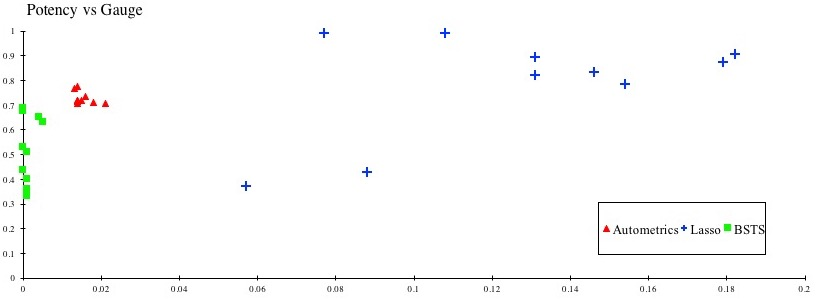
\includegraphics[scale=.5]{GPGraph}
\caption{Scatter plot of potency vs. gauge across all experiments}
\label{fig:GaugePot}


\end{figure}


\subsection{What do the Monte Carlo simulation results say about empirical model selection?}

As should be clear by now, model selection is difficult to evaluate empirically; it is impossible to judge how `good' a selected model is because it is impossible to know what to be judging against. This is why the results from MC simulations are so important and useful, and in particular why analyzing what happens when correlation structures change is vital. Because a modeller can never know what the properties of the relevant variables are, to draw valuable insight from selected models it is key that model selection not be reliant on what those properties are. With this in mind, the results in this study imply that a modeller performing model selection using the three algorithms can assume the following:

\textbf{Autometrics}
\begin{enumerate}
\item There are slightly higher than 100($\alpha$)\% of the total number of irrelevant variables included in the selected model. 
\item The probability that a variable with `significance', in signal-to-noise terms of $\psi$ has been selected can be approximated by the theoretical retention probability formula.
\item The costs of inference, or equivalently the parameter estimate accuracy, does not vary according to how `significant' a variable is. (Bias correction has not been employed here, but studies show that this a costless way of improving parameter accuracy. See Hendry and Krolzig (2005))
\item The costs of search for using Autometrics are minimal and sometimes even negative. That is, a researcher will `lose' almost nothing employing Autometrics, but stands to gain considerably.
\end{enumerate}

\textbf{Lasso}
\begin{enumerate}
\item There can be anywhere in the range of 8-20\% of the total number of irrelevant variables included in the selected model. When $N=120$, this implies keeping up to 24 irrelevant variables, compared to 6 relevant variables.
\item If all the important variables in the model happen to be relevant to the dependent variables in the same `direction' (i.e. all matter in either a positive or negative way for the dependent variable), then the Lasso will identify and select them with a high probability. In particular, a variable with a signal-to-noise ratio of $\psi>3$ has over a 97\% change of being selected.
\item The probability of selecting a relevant variable with a lower signal-to-noise ratio varies according to how correlated it is with the other variables in the model. For example the probability of selecting a variable with a signal-to-noise ratio of $\psi=2$ can be anywhere in the range of 55-98\%. 
\item Parameter estimates become increasingly inaccurate the more `significant' a variable is.
\end{enumerate}

\textbf{BSTS}
\begin{enumerate}
\item There are almost no irrelevant variables (around 0.1\%) included in the selected model.
\item This sparsity has an impact on the inability to keep relevant variables.
\item BSTS is affected by the correlation structure of the regressors, and the signs of the coefficients.
% \item another? 
\end{enumerate}

\chapter{An Application: Using Automatic Model Selection for Nowcasting}
In this chapter, automatic model selection is applied to the problem of nowcasting. It is important to note that while nowcasting may be a fruitful application of automatic model selection, nowcasting (or forecasting) is a fundamentally different problem with a different objective than model selection. While in a stationary world with no breaks the best in-sample model produces the best forecast, this is not the case in a non-stationary world. When dealing with non-stationarity, poor in-sample models can outperform in forecasting, and poor forecasting models can outperform in-sample models.  Therefore this section is included to show an interesting application of Autometrics, the Lasso and BSTS and the results should be interpreted separately from the previous section. 

\section{Google Search Query Data}

The amount of information Google collects through search queries is difficult to comprehend. According Amit Singhal, a Senior Vice President at Google, as of August 2012 Google was processing 100 billion searches every month.\footnote{According to tech blogger Danny Sullivan (2012), this was revealed by Amit Singhal at a press event in San Francisco on August 8th 2012, and is a widely quoted figure.} That means there are over 3.5 billion Google searches each day and over 1 trillion Google searches per year. People turn to Google to get information on just about every aspect of their lives, so it makes sense that Google search queries contain large amounts of information about the state of the world. It is easy to think of cases where Google search queries may contain information about macroeconomic indicators. For example, if an individual loses their job, one of the first places they are likely to go is Google to determine what their unemployment benefits are. Google is also one of the first places they would turn to begin searching for a new job. Thus, Google search queries potentially tell a story about the current state of unemployment in the economy. Similarly, individuals looking to buy new cars are likely to turn to Google to research their options before actually going to a dealership. Google search queries related to new cars could therefore provide insight into current consumer sentiment. Examples of studies which have endeavored to use Google search information for nowcasting and forecasting include D'Amuri and Marcucci (2012), Askitas and Zimmermann (2009) and Webb (2009). 

Google has recently developed several online tools, namely Google Trends and Google Correlate, which allow users to analyze what people have been Googling. Google Trends allows users to enter any search term and see the frequency with which it has been searched over time. Google Correlate allows users to enter a search query and see which other search queries are most correlated with it. Google Correlate has an additional feature which allows the user to enter their own time series and provides the user with the search queries which are most correlated with their submitted time series \cite{WhitePaper}.\footnote{Google Trends is available at \url{https://www.google.co.uk/trends} and Google Correlate is available at \url{https://www.google.com/trends/correlate}.} 

\subsection{Google Flu Trends}

One of the first ways in which the information contained in Google search query data was harnessed was with the Google Flu Trends application. The Center for Disease Control (CDC) in America publishes statistics on the proportion of doctor or hospital visits due to influenza-like illness symptoms (ILI) every week.\footnote{Data is available to download via the FluView Interactive application available at \url{ http://gis.cdc.gov/grasp/fluview/fluportaldashboard.html}} This data is a leading indicator for the prevalence of the flu in the United States. The CDC, however, releases this data at a two-week lag. By economic standards two weeks is not long; most economic statistics are released with at least this much of a lag. For flu epidemics, however, two weeks can be a long time and there can be significant costs to this delay. Action to combat the flu in the form of vaccination, research and public awareness begins later than is ideal. There is therefore obvious value in knowing about a flu outbreak or epidemic as it is beginning. Google developed the Google Flu Trends (GFT) tool with the objective of using Google search queries to accomplish exactly this. GFT produced forecasts - or more precisely nowcasts - using Google search queries to estimate the current measure of ILI. Initially, these nowcasts turned out to be surprisingly accurate.

Google stopped publishing their ILI estimates in 2014, largely because Google Flu Trends performed poorly during the 2013 flu season. While Google never fully disclosed the algorithm behind Google Flu Trends directly, the general approach was outlined in a paper in Nature \cite{naturegoogle}. In this section, Google Flu Trends is revisited, and nowcasts are made using the three algorithms already analyzed. Again, it should be stressed that while in this section automatic model selection algorithms are used to produce nowcasts, model selection itself is a fundamentally different problem, with a different objective, than forecasting or nowcasting. Thus, while nowcasting is an interesting and informative exercise, comparing model selection algorithms for their `model selecting ability' using the accuracy with which they are capable of nowcasting in these sections should be done cautiously, if at all.  
%BSTS, the algorithm analyzed in the previous section, was meant to be an improvement to the original Googel Flu Trends algorithm. 

\section{The Data}

Nowcasting ILI using automatic model selection commences in a similar way to model selection in general. The first step is to formulate the GUM, which includes all variables which may be predictors of ILI at time $t$. An important question then is to consider what data is available at time $t$ which may be relevant for nowcasting ILI. Here, the GUM includes both past ILI values, and relevant Google Correlates, which are explained in this section.

\subsection{Influenza-like-Illness Data}

As mentioned, the CDC releases weekly data on the proportion of GP visits due to influenza-like illness with a two week lag. Weeks are measured from Sunday-Saturday and are numbered either 1-52 or 1-53, depending on how many weeks are in a particular year. Week 1 in a given year is the first week which is entirely in the new year; so Week 1 2016 went from Sunday January 3-Saturday January 9th. New data is published on Fridays and gives the ILI from two weeks earlier. For example, the incidence of ILI for Week 8 2016 which went from Sunday February 21-Saturday February 27 was released on Friday in Week 10 2016 (March 4). This means that if a nowcast for ILI for Week $t$ were to be made on or after Friday of Week $t$, ILI data up to Week $t-2$ is available. Therefore, the GUM can include up until the second lag of ILI. 

\begin{figure}[h]
\centering
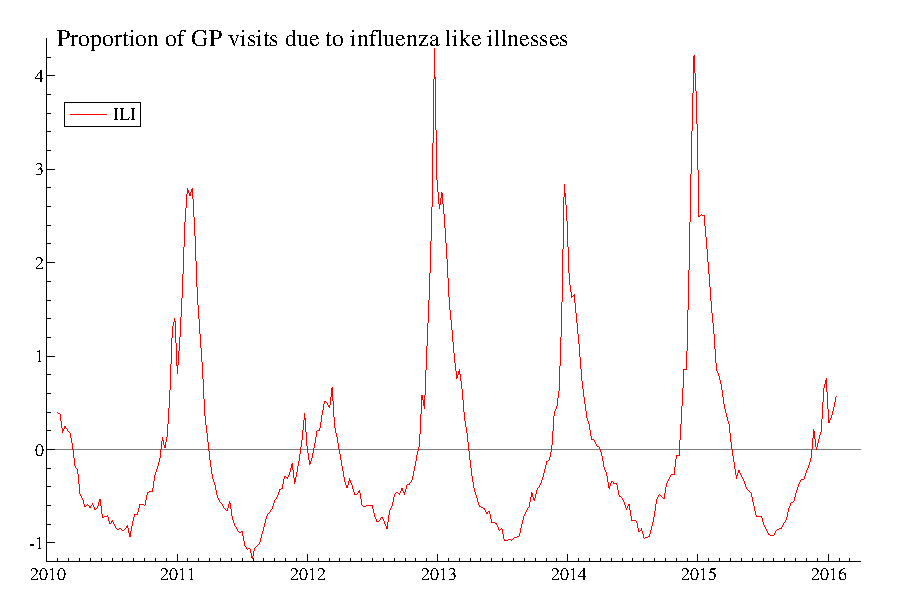
\includegraphics[scale=0.9]{ILIplot}
\caption{Proportion of GP visits due to influenza-like illness}
\label{fig:ILIplot}
\end{figure}



\subsection{Google Correlate Data}

The Google search terms which are most correlated with ILI, called the correlates, as well as their first lags, are also relevant for nowcasting. To find these correlates over a particular period, the weekly ILI time series corresponding to the desired time period was entered into the Google Correlate application. The time period differed with the two different nowcasting approaches taken, which will be explained below. Conveniently, like ILI, Google Correlate measures weeks from Sunday-Saturday. Google Correlate produces a list of the 100 search queries which are most correlated with ILI for the given sample, and also provides the de-meaned and standardized search volume for those 100 search queries as weekly time series. The search volume for a particular query is the proportion of total search queries throughout a given week which were for that query. As a practical matter, Google Correlate data is available to the public with a lag of several weeks. Acknowledging, however, that Google search query data is collected in real time, and in theory would be available for nowcasts, the nowcasting done here assumes that real time data is available. This approach is line with what was done with the original Google Flu Trends tool as well, making the results here comparable. 

\section{Nowcasting with Autometrics, Lasso and BSTS}

Nowcasting here is evaluated using both in-sample and out-of-sample results. In-sample nowcasting refers to a estimating a single model using data from the entire sample period. Fitted values for the sample period are the nowcasts. Out-of-sample nowcasting refers to selecting a holdout period, estimating a model which does not use the data from the holdout period, and using the estimated model to find fitted values for the holdout period. Finding in-sample and out-of-sample nowcasts is relatively straightforward using Autometrics and Lasso. As likely became apparent when the algorithms were described, BSTS is a much more complicated algorithm. Its main purpose, however, is nowcasting and there are features built into the BSTS R package which allow this to be done almost automatically. The reliance of BSTS on Kalman filtering and smoothing, however, means that at this point it is not capable of producing true out-of-sample nowcasts. Therefore, only in-sample nowcasts are results for BSTS.
%At a very basic level, nowcasts are made by drawing from the derived posterior distribution, and taking the mean across these draws. 

\subsection{In-sample Nowcasts using Autometrics and Lasso}
The sample period used to find in-sample nowcasts went from Week 5 2010 to Week 4 2016 (the week beginning January 31 2010 to the week beginning on January 24 2016). The ILI time series was downloaded from the CDC website for this time period, and the observations are denoted $ILI_{1},...,ILI_{313}$ since there are 313 observations in the sample period. The GUM included any variables potentially relevant for modeling ILI. A quick glance at the graph of ILI in Figure \ref{fig:ILIplot} indicates it is likely following an autoregressive process. ILI peaks in the winter around Christmas and is at its lowest in the summer, indicating that seasonality is important. Therefore, lags 2-53 of  ILI were included in the GUM. Admittedly, this is not perfect as the number of weeks in a year varies and, for example, Christmas which likely is relevant to ILI can fall in a different week year-to-year. The other set of regressors in the GUM were the top 100 correlates, and their first lags. These were found by entering the ILI time series for the sample period into the Google Correlate application.  Let $x_{1,t}, x_{2,t},...,x_{100,t}$ denote the search volumes of the top 100 correlates at time $t$. Table \ref{tab:top10correlates} shows the 10 search queries most correlated with ILI for the sample period. To give an example of the correlation structure of the Google correlates, the correlation matrix $\Omega$ of the top ten correlates is:
$$ \Omega = 
\begin{pmatrix}
 1.00  & 0.99  & 0.98  & 0.98  & 0.96  & 0.96  & 0.94  & 0.96  & 0.93  & 0.94 \\
    0.99  & 1.00  & 0.98  & 0.98  & 0.97  & 0.97  & 0.95  & 0.97  & 0.94  & 0.95 \\
    0.98  & 0.98  & 1.00  & 1.00  & 0.96  & 0.96  & 0.94  & 0.95  & 0.93  & 0.94 \\
    0.98  & 0.98  & 1.00  & 1.00  & 0.96  & 0.96  & 0.94  & 0.96  & 0.93  & 0.94 \\
    0.96  & 0.97  & 0.96  & 0.96  & 1.00  & 0.97  & 0.92  & 0.96  & 0.94  & 0.93 \\
    0.96  & 0.97  & 0.96  & 0.96  & 0.97  & 1.00  & 0.93  & 0.96  & 0.95  & 0.93 \\
    0.94  & 0.95  & 0.94  & 0.94  & 0.92  & 0.93  & 1.00  & 0.92  & 0.96  & 0.99 \\
    0.96  & 0.97  & 0.95  & 0.96  & 0.96  & 0.96  & 0.92  & 1.00  & 0.93  & 0.93 \\
    0.93  & 0.94  & 0.93  & 0.93  & 0.94  & 0.95  & 0.96  & 0.93  & 1.00  & 0.95 \\
    0.94  & 0.95  & 0.94  & 0.94  & 0.93  & 0.93  & 0.99  & 0.93  & 0.95  & 1.00 \\

  \end{pmatrix}
$$
\begin{table}
\centering
\begin{tabular}{r|r|r}
\textbf& \textbf{Search query} & \textbf{Correlation with ILI}\\
\hline
$x_{1}$& how to get over the flu & 0.942\\
$x_{2}$&get over the flu	&0.942\\
$x_{3}$&how to get rid of the flu	& 0.932\\
$x_{4}$&get rid of the flu & 0.927	\\
$x_{5}$&flu fever	&0.925\\
$x_{6}$&flu duration	& 0.924\\
$x_{7}$&type a influenza	&0.924\\
$x_{8}$&getting over the flu	&0.919\\
$x_{9}$&tamiflu and pregnancy&	0.918\\
$x_{10}$&influenza type a& 0.917\\
    \end{tabular}%
      \caption{Top 10 correlates and their correlation with ILI}
  \label{tab:top10correlates}%
\end{table}%

The top 100 correlates, their first lags, and the lagged $ILI_{t}$, formed the GUM:
$$ILI_{t}= \alpha + \sum_{i=2}^{53}\gamma_{i}ILI_{t-i}+ \sum_{i=0}^{1}\sum_{j=1}^{100}\beta_{j,i}x_{j,t-i}+u_{t}$$
Autometrics and the Lasso were applied to the above GUM. A significance level $\alpha$ must be selected when using Autometrics, and it is not immediately clear which level should be chosen in this case. This problem is discussed in more detail below, but $\alpha=0.01$ was used. Autometrics returned a model which had 60 parameters selected. Using 10-fold cross validation to select the tuning parameter $\lambda$, Lasso selected a model with 29 parameters. The nowcasts produced by Autometrics and the Lasso are the fitted values, and are plotted against ILI in Figure \ref{ig:InSample}. Table \ref{tab:selvars} displays the mean squared errors, as calculated by:
$$ MSE = \frac{1}{52}\sum_{t=262}^{313}(ILI_{t} - \widehat{ILI_{t}})^{2}$$
where $\widehat{ILI_{t}}$ is the fitted value for ILI at time $t$. Since nowcasts were made for the week of February 1 2015 to the week of January 24 2016, there are 52 nowcasts in total, denoted $\widehat{ILI}_{262},...,\widehat{ILI}_{313}$ to reflect that they correspond to the last 52 observations in the sample. 


\subsection{In-sample Nowcasts using BSTS}
While it is fairly easy to understand how Autometrics and the Lasso calculate their nowcasts, BSTS is more complicated. BSTS deals with time series components and regression components separately, so the first step is determining which time series components, and which regression components to include in the system. Based on the graph of ILI in Figure \ref{fig:ILIplot}, a local linear trend, and seasonal component with $S=53$ are used to model the time series dynamics. The regression component consists of the 100 Google correlates and their first lags, denoted by $\mathbf{x_{t}}$ and $\mathbf{x_{t-1}}$ respectively. Using the state space representation as earlier, ILI can then be described by the following system, which is summarized by `time series + regression components':
\begin{align*}
ILI_{t} &= \mu_{t} + \tau_{t} + \beta_{1}'\mathbf{x_{t}} +\beta_{2}'\mathbf{x_{t-1}} + \epsilon_{t}\\
\mu_{t} &= \mu_{t-1} + \gamma_{t-1} + u_{t}\\
\gamma_{t} &= \gamma_{t-1} + v_{t}\\
\tau_{t} &= - \sum_{s=1}^{52} \tau_{t-s} + w_{t}
\end{align*}
Operationally, BSTS first determines `how much' of $ILI_{t}$ is explained by the local linear trend and seasonality components using Kalman filtering, smoothing and Bayesian data augmentation. Thus, the following system is relevant for the time series component of the algorithm:
\begin{align*}
ILI_{t} &= \mu_{t} + \tau_{t} + \epsilon_{t}\\
\mu_{t} &= \mu_{t-1} + \gamma_{t-1} + u_{t}\\
\gamma_{t} &= \gamma_{t-1} + v_{t}\\
\tau_{t} &= - \sum_{s=1}^{52} \tau_{t-s} + w_{t}
\end{align*}
which is exactly as above, but with the regression component subtracted out. BSTS subtracts the time series component from ILI to end up with $ILI^*$. Then a spike-and-slab regression is used with $ILI^*$ as the dependent variable to determine which of the Google correlates (and their first lags) are relevant for explaining what is not explained by time series components. From the results of the spike-and-slab regression the posterior inclusion probabilities are calculated for each of the Google correlates. Figure \ref{fig:flutrendscomponents} provides a graphical illustration of the contributions of each state. Note that the lines are fuzzy because the draws are graphed. Figure \ref{fig:inclprob} shows Google correlates which have posterior inclusion probability greater than 0.15.

\begin{figure}
\centering
\includegraphics[scale=.8]{bsts-components-flutrends}
\caption{Contributions to ILI by state}
\label{fig:flutrendscomponents}
\end{figure}

\begin{figure}
\centering
\includegraphics[scale=0.5]{bsts-inclusionprob-flutrends}
\caption{Posterior inclusion probabilities for $p>0.15$. White bars indicate the coefficient sign is positive and black bars indicate the coefficient sign is negative.}
\label{fig:inclprob}
\end{figure}


As a Bayesian algorithm, BSTS does not, in fact, calculate fitted values; it derives the predictive posterior distribution for the response variable, and subsequently produces a sample of draws from this distribution \cite{bstspaper}. Nowcasts can then be found by taking the mean across these draws. Figure \ref{ig:InSample} graphs the BSTS nowcasts and Table \ref{tab:selvars} shows the mean squared errors of these nowcasts.
  
\subsection{Comparing In-Sample Nowcasts}

Looking at the graphs in Figure \ref{ig:InSample}, all three algorithms produce reasonably accurate nowcasts. Of the three, the Lasso seems to struggle the most. This is confirmed by the MSEs in Table \ref{tab:selvars}. The number of regressors selected by each of the algorithms, or in the case of BSTS, the number of variables with inclusion probability greater than 0.15, is also shown in Table \ref{tab:selectedvars}. Table \ref{tab:selvars} provides a full list of the variables selected by each algorithm.

Autometrics has the smallest MSE and selects the largest number of variables with 60 of the 252 possible variables selected. BSTS identifies only 10 variables which have posterior inclusion probabilities greater than 0.15. Comparatively, the Lasso's nowcasts are decidedly less accurate. The fact that the Lasso selected half as many variables as Autometrics seems to point to a situation where there is high degree of correlation between the regressors, and where some of these variables are relevant in opposite ways.
The table and graphs show that while all three algorithms are reasonably effective and nowcast with a high degree of accuracy, Autometrics does particularly well. 
%BSTS niter = 4000
\begin{table}
\centering
\begin{tabular}{r|r|r}
 & \textbf{MSE} & \textbf{Variables Selected}\\
 \hline
\textbf{Autometrics} & 0.003 & 60 \\
\textbf{Lasso} & 0.008 & 26\\
\textbf{BSTS} & 0.004 & 10\\
    \end{tabular}%
      \caption{MSEs from in-sample nowcasting}
  \label{tab:selvars}%
\end{table}%



\begin{figure}[h]
\centering
\includegraphics[scale=.95]{All3IS}
\caption{In-sample nowcasts}
\label{ig:InSample}
\end{figure}

% Table generated by Excel2LaTeX from sheet 'compare'
\begin{table}
\small
\singlespacing
  \centering

    \begin{tabular}{l  | l  | l}
    \textbf{BSTS} & \textbf{Lasso} & \textbf{Autometrics} \\
    \hline
    flu type a_1 & anas barbariae & anas barbariae \\
    cough fever& breaking a fever & breaking a fever \\
    get rid of the flu& cold fever & child with flu \\
   home remedies for flue & cough fever & cold fever \\
  cough rememdies  & cough remedies & cold or flu \\
   tamiflu dose & cure a cough & cough fever_1 \\
   flu how long & dangerous fever & cure a cough \\
    is the flu contagious& flu medicines & cure a cough_1 \\
    how to cure the flu& flu medicines_1 & dangerous fever \\
   how long does fever last with flu  & ILI_14 & flu a \\
	 & ILI_15 & flu a_1 \\
    & ILI_16 & flu aches \\
    & ILI_17 & flu aches_1 \\
     & ILI_2 & flu and pregnancy \\
     & ILI_28 & flu how long_1 \\
   & ILI_29 & flu recovery \\
    & ILI_3 & flu remedies_1 \\
     & ILI_50 & flu treatments \\
    & ILI_51 & flu type a \\
     & influenza treatment_1 & flu type a_1 \\
    & tamiflu and breastfeeding & generic tamiflu_1 \\
    & tamiflu drug_1 & get rid of the flu \\
    & tamiflu pediatric dosing & home remedies for flu \\
     & tamiflu side effects & how long contagious \\
     & treat a fever & how long does fever last with flu \\
     & type a flu & how long does it take to get over the flu \\
     &       & how long is the flu contagious \\
     &       & how long is the flu_1 \\
   &       & how to cure the flu \\
     &       & how to cure the flu_1 \\
     &       & how to get rid of flu_1 \\
     &       & how to treat the flu_1 \\
     &       & ILI_2 \\
    &       & ILI_3 \\
          &       & ILI_30 \\
          &       & ILI_4 \\
          &       & ILI_5 \\
          &       & ILI_6 \\
          &       & ILI_9 \\
          &       & influenza a_1 \\
          &       & influenza type a \\
          &       & is the flu contagious \\
          &       & is the flu contagious_1 \\
          &       & medicine for the flu_1 \\
          &       & over the counter flu \\
          &       & remedies for flu_1 \\
          &       & symptoms of pneumonia \\
          &       & tamiflu and alcohol_1 \\
          &       & tamiflu and pregnancy \\
          &       & tamiflu and pregnancy_1 \\
          &       & tamiflu drug_1 \\
          &       & tamiflu side effects \\
          &       & treat a fever \\
          &       & treat a fever_1 \\
          &       & treat the flu \\
          &       & treat the flu_1 \\
          &       & treating the flu_1 \\
          &       & type a flu_1 \\

    \end{tabular}%
      \caption{Selected regressors}
  \label{tab:selectedvars}%
\end{table}%

\subsection{Out-of-sample Nowcasting with Autometrics and the Lasso}

In-sample nowcasting or forecasting where the GUM is the starting point obviously has the potential to be very accurate due to the fact that the training set and the validation set are the same. The example of an extreme case of using OLS when $T=N$, and the fitted values exactly correspond to the true values comes to mind. It is important to consider how nowcasts perform out-of sample, as this reflects the situation in which nowcasts would be made in reality.  A nowcast for time $t$ is based on a model estimated using only the information available at $t$ is a better reflection of how nowcasting would be useful in practice.

To calculate out-of-sample nowcasts using automatic model selection there are several decisions that need to be made. First it must be decided whether the algorithm should reselect a model from the GUM for each successive nowcast. If a new model is estimated for each successive nowcast, another question is whether a rolling or recursive window is more appropriate for determining the sample period. An issue specific to using Google Correlates is whether a new set of correlates should calculated from the Google Flu Trends application for each new nowcast. 

The following explanation is easier to understand with reference to Table \ref{fig:cal}. The chosen sample period went from Week 5 2010 to Week 4 2016 (the week beginning January 31 2010 to the week beginning on January 24 2016) from which there are 313 observations. The `modified holdout' period for which nowcasts were made went from Week 5 2015 and Week 4 2016 (the week beginning February 01, 2015 to the week beginning January 24, 2016). These nowcasts are denoted $\widehat{ILI}_{262},...,\widehat{ILI}_{313}$.  The top 100 Google correlates were found by entering the ILI time series for the sample period excluding the holdout period ($ILI_{1},...,ILI_{261}$) into the Google Correlate application. The top 100 Google correlates are denoted $x_{1,t},...,x_{100,t}$. Variables were selected once and selection was made using only the data in the subsample which excluded the holdout period. So, variables were selected from the following GUM:
$$ILI_{t}= \alpha + \sum_{i=2}^{53}\gamma_{i}ILI_{t-i}+ \sum_{i=0}^{1}\sum_{j=1}^{100}\beta_{j,i}x_{j,t}+u_{t}$$
for $t=1,...,261$. The model estimated from the GUM was used to produce the first nowcast, for the week of Feb 1, 2015, denoted $\widehat{ILI}_{262}$. The reason why the holdout period is `modified' is because for each successive nowcast, an additional observation was added to the sample and a new model was estimated by OLS. The variables included in this model were the variables initially selected by the GUM. Let $z_{1},...,z_{L}$ denote the $L$ regressors selected initially from the GUM. Nowcast $\widehat{ILI}_{262+k}$ was found by estimating the following model, for k=1,..,51:
$$ILI_{t}= \alpha + \sum_{i=1}^{L}\xi_{i}z_{i,t}+ v_{t}, \hspace{1cm} t=1,...,262+k$$
Therefore, new estimates for the $\xi_{i}$s were made to find the new model used to produce each nowcast. The fitted value $\widehat{ILI}_{262+k}$ from the $k^{th}$ model estimated is the nowcast. This process was used for both Autometrics and the Lasso. For Autometrics, the significance level $\alpha$ was set to $0.01$. In the case of Lasso, selecting variables once and using OLS with the selected variables as the regressors for the subsequent nowcasts is equivalent to setting the tuning parameter $\lambda = 0$. The nowcasts and ILI produced by Autometrics and Lasso are graphed in Figure \ref{fig:OutofSample}. The nowcast MSEs, and the number of variables selected by each algorithm is in Table \ref{MSEoutofsample}. Autometrics and Lasso perform similarly, with Lasso achieving a slightly smaller MSE than Autometrics. 
\begin{table}[h]
\centering
\begin{tabular}{r|r|r}
 & \textbf{MSE}& \textbf{Variables Selected} \\
 \hline
\textbf{Autometrics} & 0.016 & 33\\
\textbf{Lasso} & 0.014 & 30 \\
\hline
\textbf{Average} & 0.005 &\\

    \end{tabular}%
      \caption{MSEs from out-of-sample nowcasting}
  \label{MSEoutofsample}%
\end{table}%


The in-sample nowcast graphs indicate that the Autometrics nowcasts tend to be above the true ILI, and that the Lasso's tend to be below the true ILI. A graph of the residuals in Figure \ref{fig:nowcastresiduals} makes this a little clearer. This suggests that perhaps the average of the two nowcasts would produce an even more accurate nowcast. Let $\widehat{ILI}_{ave, t}$ denote this average, $\widehat{ILI}_{auto, t}$ denote the Autometrics nowcast and $\widehat{ILI}_{lasso, t}$ denote the Lasso nowcast as calculcated above. The new average nowcast for time $t$ is:
$$\widehat{ILI}_{ave, t} = \frac{1}{2}(\widehat{ILI}_{auto, t} + \widehat{ILI}_{lasso, t})$$
The average nowcast is also graphed against ILI in Figure \ref{fig:OutofSample}. The MSE of the average is 0.005, which is less than half the MSE of both Autometrics and Lasso individually.  
\afterpage{
\begin{figure}
\includegraphics[scale=.9]{BothPlots}
\caption{Out-of-sample Nowcasts}
\label{fig:OutofSample}
\end{figure}

\begin{figure}
\centering
\includegraphics[scale=.9]{nowcastresiduals}
\caption{Residuals from Autometrics and Lasso nowcasts}
\label{fig:nowcastresiduals}
\end{figure}
}
\afterpage{
\begin{landscape}
\begin{figure}
\centering
\includegraphics{Calendar}
\caption{The timing of in-sample nowcasts and ILI releases}
\label{fig:cal}
\end{figure}
\end{landscape}
}


\subsection{Predicting ILI with Autometrics and the Lasso}

Given that both Autometrics and the Lasso seem reasonably effective at producing accurate nowcasts, an interesting question is whether actual predictions of ILI would be useful. To test this, forecasts of ILI were made using Autometrics and the Lasso.
The forecasting here was done in much the same way as nowcasting was done in the previous section. The sample period from Week 5 2010 to Week 4, 2016 (the week beginning January 31 2010 to the week beginning on January 24 2016) from which there are 313 observations. Forecasts were made for the 52 weeks between Week 5 2015 and Week 4 2016 (the week beginning February 01, 2015 to the week beginning January 24, 2016), and are denoted $\widetilde{ILI}_{262},...,\widetilde{ILI}_{313}$. The top 100 Google correlates were found by entering the $ILI_{t+1}$ time series for the sample period into the Google Correlate application. These correlates, then, are the search terms at time $t$ which are most correlated with ILI at $t+1$ and are denoted $x_{1,t}^{*},...x_{100,t}^{*}$. Again, variables were only selected once, using only the data in the sample period. Thus, the initial model was selected from the GUM:
$$ILI_{t+1}= \alpha + \sum_{i=2}^{53}\gamma_{i}ILI_{t-i}+ \sum_{i=0}^{1}\sum_{j=1}^{100}\beta_{j,i}x_{j,t-i}^{*}+u_{t}$$
The significance level was again set to $\alpha = 0.01$ for Autometrics. The first forecast was made for $ILI_{262}$ and was produced using the model selected from GUM. The fitted value $\widetilde{ILI}_{262}$ from this model is the reported forecast.  For the 51 subsequent forecasts, OLS was used to re-estimate a model using the variables selected by the GUM, and using the information available at the time the forecast was made. For example, the forecast for $ILI_{263}$ was made using information available at $t=262$. If $z_{1},...,z_{L}$ were $L$ the variables selected from the GUM, then to produce $\widetilde{ILI}_{262+k}$, the following model was estimated by OLS:
$$ILI_{t+1}= \alpha + \sum_{i=1}^{L}\xi_{i}z_{i,t}+ v_{t}, \hspace{1cm}  t=1,...,260+k$$
The $k$ fitted values for $ILI_{t+1}$ from each of the $k$ models estimated are the reported forecasts. The forecasts are plotted in Figure \ref{fig:Forecasts}, and the MSEs are reported in Table \ref{tab:MSEforecasts}. The forecasts produced by Autometrics are noticeably less accurate than the nowcasts. The Lasso performs nearly as well at forecasting as it does at nowcasting. The average is better than both, Autometrics and Lasso individually, though only marginally better than the Lasso. 



\begin{figure}[h]
\centering
\includegraphics{forecastplot}
\caption{Forecasts produced by Autometrics, Lasso, and their average.}
\label{fig:Forecasts}
\end{figure}


\begin{table}[h]
\centering
\begin{tabular}{r|rr}
 & \textbf{MSE} &\textbf{Selected Variables} \\
 \hline
\textbf{Autometrics} & 0.032 & 41\\
\textbf{Lasso} & 0.018 & 22 \\
\hline
\textbf{Average} & 0.016 &  \\
    \end{tabular}%
      \caption{MSEs from forecasting}
  \label{tab:MSEforecasts}%
\end{table}%












\subsection{Original Google Flu Trends Estimates}

Since its inception in 2008, the Google Flu Trends model has been updated three times, most recently in 2014. While Google has never released the algorithm it used to compute its ILI estimates, the estimates themselves are available. It has also released the estimates that the revised models produce when applied to historical data.\footnote{ILI estimates from all versions of the Google Flu Trend algorithm can be downloaded from \url{https://www.google.org/flutrends/about/}}. An interesting exercise is then to see how these estimates compare to the estimates produced using the algorithms studied here. 

Figure \ref{fig:2014GFT} graphs the nowcasts produced by Google's 2014 model, for the period January 24, 2010 until October 19 2015 which is the last estimate available.\footnote{The estimates in this graph were downloaded on March 21st from \url{https://www.google.org/flutrends/about/data/flu/historic/us-historic-v3.txt}} Note that it is not clear whether these are in-sample or out-of-sample nowcasts. The nowcast MSE over this period is 0.021, which is larger than the in-sample MSEs for Autometrics, Lasso and BSTS, and the out-of-sample nowcast MSEs produced by Autometrics and the Lasso. 


\begin{figure}
\centering
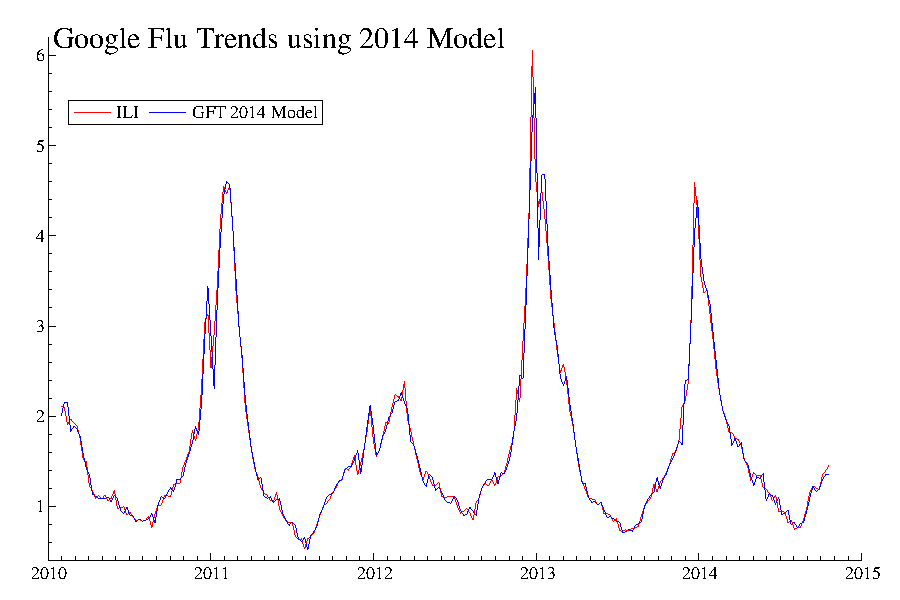
\includegraphics[scale=.8]{GFT2014}
\caption{Nowcasts for 2010-2015 using Google's 2014 model}
\label{fig:2014GFT}
\end{figure}


\section{Selecting the Significance Level for Autometrics}

The accuracy of the nowcasts and forecasts produced by the three different algorithms has been measured by the MSE, which measures how close the predictions and true values are. Clearly, this is a very different way to evaluate the algorithms than the gauge, potency and MSE measures which were used in Chapter 3. When using Autometrics there is strong relationship between the chosen significance level $\alpha$ and the inclusion of irrelevant variables. Approximately $100(\alpha)\%$ of the irrelevant variables present in the GUM are in the model selected by Autometrics. The selection of relevant variables is also influenced by $\alpha$; a higher $\alpha$ means a lower critical value $c_{\alpha}$ which leads to more relevant variables selected. Therefore, when selecting $\alpha$ there exists a tradeoff between setting a low $\alpha$ and excluding most of the irrelevant variables and retaining fewer of the relevant variables, or selecting a high $\alpha$, and retaining most relevant variables, while simultaneously retaining many irrelevant variables. When the goal of using Autometrics is model selection, the consensus is that setting $\alpha$ very low is preferable. However when the goal is not model selection but is instead forecasting, setting a higher $\alpha$ could produce better results. This is due to the fact that in the prediction arena, it is sometimes more costly to exclude relevant variables than it is to retain irrelevant variables. There is a long debate over parsimony versus robustness and it is far from settled, but given that excluding relevant variables is perhaps more costly than including irrelevant variables, it seems sensible to entertain the idea that higher values of $\alpha$ could improve nowcasts and forecasts generated by Autometrics.  
Out-of-sample nowcasts and forecasts were reproduced with this in mind, using the out-of-sample nowcasting and forecasting methods as previously explained, with various values of $\alpha$. The MSE results for the recalculated nowcasts are reported in Table \ref{tab:MSENowcastsdiffalpha}, and results for the recalculated forecasts are reported in Table \ref{tab:MSEForecastdiffalpha}. Averages calculated using the updated nowcasts and forecasts are also reported.  Both the nowcasts and forecasts produced by Autometrics generally improve with the higher levels of significance. 




\begin{table}[h]
\centering

\begin{tabular}{r|r|r|r}
   $\bf{\alpha}$    & \textbf{Autometrics} & \textbf{Average} & \textbf{Variables Selected} \\
  \hline
0.01 &     0.016                                &     0.005           &          33                   \\
0.05 &      0.018                        &     0.005             & 59\\
0.10 &      0.012                                  &    0.008         &62       \\
0.15 &    0.012                                     &     0.005       &   91 \\
0.20&        0.012                              &          0.006     &        92                    
\end{tabular}
\caption{Nowcast MSEs for various levels of $\alpha$}
\label{tab:MSENowcastsdiffalpha}
\end{table}

\begin{table}[h]
\centering

\begin{tabular}{r|r|r|r}
   $\bf{\alpha}$    & \textbf{Autometrics} & \textbf{Average} &\textbf{Variables Selected} \\
  \hline
0.01 &  0.032                         &                0.016            &      41          \\
0.05 &  0.025                         &             0.014     & 48\\
0.10 &     0.015                	    &          0.009         & 73\\
0.15 &   0.017                        &         0.012     & 140\\
0.20 &     0.007      		 &            0.008       &     161                      
\end{tabular}
\caption{Forecast MSEs for various levels of $\alpha$}
\label{tab:MSEForecastdiffalpha}
\end{table}


%\subsection{A Side Note on Bias Correction}

%As explained in Hendry and Krolzig (2005), selection results in biased coefficient estimates. Estimates for relevant variables are biased away from zero since selection depends on $t^{2} > c_{\alpha}^2$. Some relevant variables, particularly if they are `marginally significant' and have low non-centralities, will have $t^2 < c_{\alpha}^2$ and will not be selected. Similarly, some irrelevant variables will be selected as a result $t^2 >c_{\alpha}^2$. This bias can be accounted for using the bias correction method developed by Hendry and Krolzig (2005). Numerous simulation studies have found that bias-correction results in more accurate parameter estimates. 

%Bias correction on the parameters used to produce the nowcasts and forecasts was attempted, however the results turned out to be far less accurate and therefore were not reported.  At first it seemed this could be due to the fact that the bias-correcting mechanism is meant to be used when the variables are orthogonal, and the Google correlates exhibit a high degree of correlation. To account for this, the principal components of the Google Correlates were found. While the bias corrected MSEs improved when using principal components, they were still less accurate than the MSEs where no there was no attempt to bias correct. 

%This is a bit of a puzzle. It could be due to the fact that
%Bias-correction is meant to fix the problem of adventitiously selecting irrelevant variables. In the case of using correlates to predict 

%Higher values of $\alpha$ in Autometrics results in more more variables being selected overall due to a higher critical value and cut-off threshold; this is seen easily with the increasing number of selected variables as $\alpha$ increases in both Table \ref{tab:MSENowcastsdiffalpha} and \ref{tab:MSENowcastsdiffalpha}. To account for this, Hendry and Krolzig (2005) advocate a bias correction mechanism which adjusts parameter estimates downward, to account for the fact that certain irrelevant variables are likely to be included in the selected model. 
%Acknowledging that some irrelevant variables will be adventitiously selected given the higher value of $\alpha$, and considering the high numbers of selected variables, it also seems sensible to employ the bias-correcting mechanism advocated by Hendry and Krolzig (2005),  Since the bias correction mechanism only works in the case of orthogonal variables, and the Google Correlates exhibit a high degree of correlation, the Google Correlates are transformed into their Principal Components.  Due to the high correlation between variables in this setting, it is also necessary to use 


%\subsection{Bias correction}

%As explained in Hendry and Krolzig (2005), selection results in biased coefficient estimates. Estimates for relevant variables are biased away from zero since selection depends on $t^{2} > c_{\alpha}^2$. Some relevant variables, particularly if they are `marginally significant' and have low non-centralities, will have $t^2 < c_{\alpha}^2$ and will not be selected. Similarly, some irrelevant variables will be selected as a result $t^2 >c_{\alpha}^2$. Fortunately, this bias can be accounted for using the bias correction method developed by Hendry and Krolzig (2005). As outlined earlier, the expected t-statistic for a particular variable can be characterized by its non-centrality $\psi$:
%$$ t_{\widehat{\beta}} = \frac{\widehat{\beta}}{\widehat{\sigma_{\beta}}} \simeq \frac{\widehat{\beta}}{\sigma_{\beta}} \sim N[\psi, 1]$$

%Since relevant variables which are selected will be biased away from zero, their t-statistics will be biased in the same direction. This is seen through the expression for the expected t-value of a variable after that variable has been selected. Letting  $\phi(x)$ denote the normal density, and  $\Phi(x)$ denote its integral:

%\begin{align*}
%\psi^* = E[t_{\widetilde{\beta}} |  | t_{\widetilde{\beta}} | > c_{\alpha} ; \psi ] &= \psi + \frac{\phi(c_{\alpha} - \psi) - \phi(-c_{\alpha} - \psi)}{\Phi(c_{\alpha} - \psi) - \Phi(-c_{\alpha} - \psi)}  = \psi + r(\psi, c_{\alpha})\\
%\sigma_{\widetilde{\beta}}E[t_{\widetilde{\beta}} |  | t_{\widetilde{\beta}} | > c_{\alpha} ; \psi ] &= \beta + \sigma_{\widetilde{\beta}}r(\psi, c_{\alpha})\\
%\end{align*}
%since $\beta$ is the unbiased estimator, after estimation an unbiased estimator is given by:
%$$\widetilde{\widetilde{\beta}} = \widetilde{\beta}\frac{\psi}{\psi + r(\psi, c_{\alpha}} $$
%and since
%$$\psi^* = \psi +r(\psi, c_{\alpha})$$
%then (...) add in more steps from Castle et al.
%The bias corrected estimate of $\beta$ is:
%$$ \widetilde\widetilde{\beta} = \widetilde{\beta}\frac{\widetilde{\widetilde{t}}_{\widetilde{\beta}}}{t_{\widetilde{\beta}}}$$


\section{Nowcasting Takeaways}

As this chapter shows, nowcasting is an interesting, relevant and useful application of automatic model selection and depending on the complexity of the algorithm, it can also be employed very easily. As the way that economic data is collected begins to change, and as it starts to become available in real-time, automatic model selection for nowcasting could become a  useful tool for economics, statistical agencies and policy makers alike.  

\chapter{Conclusion}
Automatic model selection algorithms have the potential to assist economic researchers a great deal. As the big data revolution starts to play a more integral role in economic research, algorithms like Autometrics, the Lasso and BSTS will become more mainstream. The results of this thesis demonstrate that while the three algorithms have broadly the same goal of selecting a sparse model from a much more general model, the properties of each algorithm vary. Of particular relevance to the results is the correlation structure of the DGP. Because empirically the structure of the DGP is impossible to know it should be viewed unfavourably if an algorithm's properties depend on a particular correlation structure.

This thesis began by first outlining the theory behind the three different algorithms studied. Then, results from simulations conducted across three different correlation structures were presented individually. Within each of these three sets of simulations, different non-centralities for the relevant variable were tested. Also examined was the impact of including more variables than observations in the initial GUM. Algorithms were compared to each other and against a benchmark to examine the costs of search and costs of inference. Finally the results across different correlation structures were analyzed.   

Of the three algorithms studied, Autometrics was found to be by the far the most consistent across correlation structures. The Lasso's results vary a great deal depending on the correlation structure and the non-centralities  of the relevant variables. This makes it difficult to describe the general properties of a model the Lasso selects. BSTS selects very sparse models overall, with the properties of the selected model dependent on the correlation structure as well. The number of candidate variables did not seem to matter in any of the algorithms; that is in most simulations, each algorithm was just as effective when the number of variables exceeded the number of observations. 

A nowcasting application of automatic model selection was then considered, where each of the algorithms was used to nowcast the incidence of the flu in the United States, using information from Google search queries. All three algorithms generated very good in-sample nowcasts. The out-of-sample nowcasts were also very accurate. Autometrics and the Lasso were also used to try to forecast the flu, with success. The results were compared to actual Google Flu Trends estimates, and were shown to be even more accurate. The results in this section suggest that nowcasting and forecasting may be a profitable application of automatic model selection algorithms. However given that the goal of nowcasting is to minimize predictive error, more work needs to be done to understand the best way to use automatic model selection in the nowcasting arena.  

The research presented in this thesis has demonstrated that if economists wish is to effectively and appropriately take advantage of the new tools for big data like the ones presented here, it is essential they do their research. The results demonstrate that not all algorithms are created equally, and that choosing one technique over another can have a significant impact on results. That said, the results in this thesis suggest that Autometrics is a promising, consistent and reliable algorithm and has the potential to greatly simplify the work of empirical researchers. 



\nocite{hendryjohansensantos}
\nocite{johansennielsen2009}
\nocite{ridgeregression70}
\nocite{spikeandslab}
\nocite{doornik2009}
\nocite{evalmodelsel}
\nocite{lassovauto}
%\nocite{campos2009}
\nocite{bstspaper}
\nocite{hendrykrolzig1999}
\nocite{hendrykrolzig2005}
\nocite{tibshirani}
\nocite{degreesoffreedomlasso}
\nocite{chechen}
\nocite{efronetal2004}
\nocite{zhangetal}
\nocite{kalmanfilter}
\nocite{introstatisticallearning}
\nocite{durbinkoopman2001}
\nocite{hendrydoornikbook}
\nocite{castleshephard2009}
\nocite{robertcasella2004}
\nocite{renfro2009}
\nocite{georgemcculloh}
\nocite{carterkohn2004}
\nocite{EricDFHSH14MF}
\nocite{WUBRYN2013}
\nocite{WEBB2009}
\nocite{CDHPSIS15}
\nocite{zouhastie}
\nocite{WhitePaper}

\bibliographystyle{apalike}
\bibliography{references}
\renewcommand*{\bibname}{Literaturliste}





\end{document}